\documentclass[twoside]{book}

% Packages required by doxygen
\usepackage{fixltx2e}
\usepackage{calc}
\usepackage{doxygen}
\usepackage[export]{adjustbox} % also loads graphicx
\usepackage{graphicx}
\usepackage[utf8]{inputenc}
\usepackage{makeidx}
\usepackage{multicol}
\usepackage{multirow}
\PassOptionsToPackage{warn}{textcomp}
\usepackage{textcomp}
\usepackage[nointegrals]{wasysym}
\usepackage[table]{xcolor}

% Font selection
\usepackage[T1]{fontenc}
\usepackage[scaled=.90]{helvet}
\usepackage{courier}
\usepackage{amssymb}
\usepackage{sectsty}
\renewcommand{\familydefault}{\sfdefault}
\allsectionsfont{%
  \fontseries{bc}\selectfont%
  \color{darkgray}%
}
\renewcommand{\DoxyLabelFont}{%
  \fontseries{bc}\selectfont%
  \color{darkgray}%
}
\newcommand{\+}{\discretionary{\mbox{\scriptsize$\hookleftarrow$}}{}{}}

% Page & text layout
\usepackage{geometry}
\geometry{%
  a4paper,%
  top=2.5cm,%
  bottom=2.5cm,%
  left=2.5cm,%
  right=2.5cm%
}
\tolerance=750
\hfuzz=15pt
\hbadness=750
\setlength{\emergencystretch}{15pt}
\setlength{\parindent}{0cm}
\setlength{\parskip}{3ex plus 2ex minus 2ex}
\makeatletter
\renewcommand{\paragraph}{%
  \@startsection{paragraph}{4}{0ex}{-1.0ex}{1.0ex}{%
    \normalfont\normalsize\bfseries\SS@parafont%
  }%
}
\renewcommand{\subparagraph}{%
  \@startsection{subparagraph}{5}{0ex}{-1.0ex}{1.0ex}{%
    \normalfont\normalsize\bfseries\SS@subparafont%
  }%
}
\makeatother

% Headers & footers
\usepackage{fancyhdr}
\pagestyle{fancyplain}
\fancyhead[LE]{\fancyplain{}{\bfseries\thepage}}
\fancyhead[CE]{\fancyplain{}{}}
\fancyhead[RE]{\fancyplain{}{\bfseries\leftmark}}
\fancyhead[LO]{\fancyplain{}{\bfseries\rightmark}}
\fancyhead[CO]{\fancyplain{}{}}
\fancyhead[RO]{\fancyplain{}{\bfseries\thepage}}
\fancyfoot[LE]{\fancyplain{}{}}
\fancyfoot[CE]{\fancyplain{}{}}
\fancyfoot[RE]{\fancyplain{}{\bfseries\scriptsize Generated by Doxygen }}
\fancyfoot[LO]{\fancyplain{}{\bfseries\scriptsize Generated by Doxygen }}
\fancyfoot[CO]{\fancyplain{}{}}
\fancyfoot[RO]{\fancyplain{}{}}
\renewcommand{\footrulewidth}{0.4pt}
\renewcommand{\chaptermark}[1]{%
  \markboth{#1}{}%
}
\renewcommand{\sectionmark}[1]{%
  \markright{\thesection\ #1}%
}

% Indices & bibliography
\usepackage{natbib}
\usepackage[titles]{tocloft}
\setcounter{tocdepth}{3}
\setcounter{secnumdepth}{5}
\makeindex

% Hyperlinks (required, but should be loaded last)
\usepackage{ifpdf}
\ifpdf
  \usepackage[pdftex,pagebackref=true]{hyperref}
\else
  \usepackage[ps2pdf,pagebackref=true]{hyperref}
\fi
\hypersetup{%
  colorlinks=true,%
  linkcolor=blue,%
  citecolor=blue,%
  unicode%
}

% Custom commands
\newcommand{\clearemptydoublepage}{%
  \newpage{\pagestyle{empty}\cleardoublepage}%
}

\usepackage{caption}
\captionsetup{labelsep=space,justification=centering,font={bf},singlelinecheck=off,skip=4pt,position=top}

%===== C O N T E N T S =====

\begin{document}

% Titlepage & ToC
\hypersetup{pageanchor=false,
             bookmarksnumbered=true,
             pdfencoding=unicode
            }
\pagenumbering{roman}
\begin{titlepage}
\vspace*{7cm}
\begin{center}%
{\Large Alps \\[1ex]\large 0.\+1.\+0 }\\
\vspace*{1cm}
{\large Generated by Doxygen 1.8.11}\\
\end{center}
\end{titlepage}
\clearemptydoublepage
\tableofcontents
\clearemptydoublepage
\pagenumbering{arabic}
\hypersetup{pageanchor=true}

%--- Begin generated contents ---
\chapter{mainpage}
\label{md__home_yuan_Benchmarks_whisper_mnemosyne-gcc_usermode_library_pmalloc_include_alps_src_mainpage}
\hypertarget{md__home_yuan_Benchmarks_whisper_mnemosyne-gcc_usermode_library_pmalloc_include_alps_src_mainpage}{}
\hypertarget{md__home_yuan_Benchmarks_whisper_mnemosyne-gcc_usermode_library_pmalloc_include_alps_src_mainpage_mainpage}{}\section{A\+L\+P\+I\+Ni\+S\+M\+: Abstraction Layer for Programming Persistent Shared Memory   }\label{md__home_yuan_Benchmarks_whisper_mnemosyne-gcc_usermode_library_pmalloc_include_alps_src_mainpage_mainpage}
A\+L\+P\+I\+Ni\+SM provides a low-\/level abstraction layer that reliefs the user from the details of mapping, addressing, and allocating persistent shared memory (also known as fabric-\/attached memory). This layer can be used as a building block for building higher level abstractions and data structures such as heaps, logs, objects, etc.

 
\begin{DoxyImage}
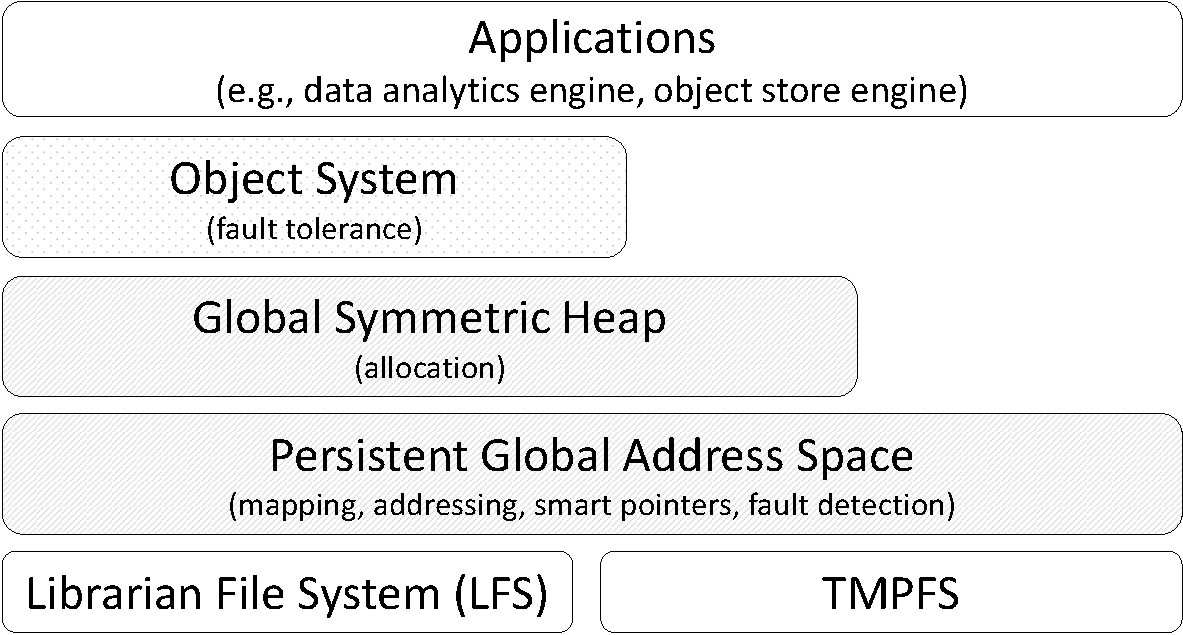
\includegraphics[width=10cm]{alps-layers}
\caption{A\+L\+P\+I\+Ni\+SM layers}
\end{DoxyImage}


Currently, we provide two layers (or A\+PI classes). First, a \hyperlink{md__home_yuan_Benchmarks_whisper_mnemosyne-gcc_usermode_library_pmalloc_include_alps_src_pegasus_pegasus_pegasuspage}{P\+Ersistent Global Address Space for Universal Sharing (P\+E\+G\+A\+S\+US)} layer provides a shared address space between multiple worker processes. Second, a Global Symmetric Heap layer for allocating variable-\/size chunks of shared persistent memory (a.\+k.\+a. fabric-\/attached memory).

The A\+P\+Is strive to be as generic as possible. Thus, we do not hardcode policy but instead seek providing generic mechanisms that can be used to support higher level policies.

\subsection*{Example Programs}

A\+L\+P\+I\+Ni\+SM comes with several samples in the {\ttfamily examples} directory.

\subsection*{This Document}

This document is written in Doxygen and maintained in the A\+L\+P\+I\+Ni\+SM git instance at\+:

\href{git://git-pa1.labs.hpecorp.net/ssftm/alps}{\tt git\+://git-\/pa1.labs.\+hpecorp.\+net/ssftm/alps}

\subsection*{Generating the documentation}

We include the A\+L\+P\+I\+Ni\+SM documentation as part of the source (as opposed to using a hosted wiki, such as the github wiki, as the definitive documentation) to enable the documentation to evolve along with the source code and be captured by revision control (currently git). This way the code automatically includes the version of the documentation that is relevant regardless of which version or release you have checked out or downloaded.

\begin{DoxyVerb} $ cd $ALPS/doc
 $ doxygen\end{DoxyVerb}


\subsection*{Reporting issues}

Please report feedback, including performance and correctness issues and extension requests, through the A\+L\+PS Jira instance\+:

\href{https://jira-pa1.labs.hpecorp.net/browse/ALPS/}{\tt https\+://jira-\/pa1.\+labs.\+hpecorp.\+net/browse/\+A\+L\+P\+S/}

\subsection*{Stable download locations}

The most recent version is published at\+: N/A

\subsection*{Contact information}

\begin{DoxyAuthor}{Author}
Haris Volos \href{mailto:haris.volos@hpe.com}{\tt haris.\+volos@hpe.\+com} 
\end{DoxyAuthor}

\chapter{pegasus}
\label{md__home_yuan_Benchmarks_whisper_mnemosyne-gcc_usermode_library_pmalloc_include_alps_src_pegasus_pegasus}
\hypertarget{md__home_yuan_Benchmarks_whisper_mnemosyne-gcc_usermode_library_pmalloc_include_alps_src_pegasus_pegasus}{}
\hypertarget{md__home_yuan_Benchmarks_whisper_mnemosyne-gcc_usermode_library_pmalloc_include_alps_src_pegasus_pegasus_pegasuspage}{}\section{P\+E\+G\+A\+S\+U\+S\+: Persistent Global Address Space for Universal Sharing       }\label{md__home_yuan_Benchmarks_whisper_mnemosyne-gcc_usermode_library_pmalloc_include_alps_src_pegasus_pegasus_pegasuspage}
A P\+Ersistent Global Address Space for Universal Sharing (P\+E\+G\+A\+S\+US) object (\hyperlink{classalps_1_1AddressSpace}{alps\+::\+Address\+Space}) provides a shared address space between multiple worker processes. The address space comprises multiple persistent memory regions, which are contiguous segments of the address space that are backed by fabric-\/attached memory (F\+AM). Each process has its own P\+E\+G\+A\+S\+US object instance that it can use to map and access shared persistent memory regions. For emulation purposes, we also provide an implementation of persistent memory regions on top of an in-\/memory file system (T\+M\+P\+FS).

Persistent regions (\hyperlink{classalps_1_1Region}{alps\+::\+Region}) are instantiated by binding and mapping region files (\hyperlink{classalps_1_1RegionFile}{alps\+::\+Region\+File}) into the address space. As each process may memory map the region file at a different location, each region type provides smart pointers (\hyperlink{group__SMARTPOINTERS}{Smart Pointers}) for referencing locations within the region in a manner that is independent of mapping address. 
\chapter{Todo List}
\label{todo}
\hypertarget{todo}{}

\begin{DoxyRefList}
\item[\label{todo__todo000001}%
\hypertarget{todo__todo000001}{}%
Class \hyperlink{classalps_1_1MemoryManager}{alps\+:\+:Memory\+Manager} ]Provide an A\+PI for picking address hints\+:
\begin{DoxyItemize}
\item best effort mapping\+: find the largest hole in the address space where we can map regions this can guide segment map to pick the right segment size
\item guide underlying OS by picking an address\+\_\+hint based on our past knowledge about persistent regions to minimize address space fragmentation similar to the Mnemosyne runtime (this could be implemented in the map method) 
\end{DoxyItemize}
\end{DoxyRefList}
\chapter{Module Index}
\section{Modules}
Here is a list of all modules\+:\begin{DoxyCompactList}
\item \contentsline{section}{Compiler Specific Optimizations}{\pageref{group__COMPILER}}{}
\item \contentsline{section}{C++11 Keywords in Public Headers}{\pageref{group__CXX11}}{}
\item \contentsline{section}{Error codes, messages, and stacktraces}{\pageref{group__ERRORCODES}}{}
\item \contentsline{section}{Smart Pointers}{\pageref{group__SMARTPOINTERS}}{}
\end{DoxyCompactList}

\chapter{Hierarchical Index}
\section{Class Hierarchy}
This inheritance list is sorted roughly, but not completely, alphabetically\+:\begin{DoxyCompactList}
\item \contentsline{section}{alps\+:\+:Address\+Space}{\pageref{classalps_1_1AddressSpace}}{}
\item \contentsline{section}{alps\+:\+:Backtrace\+Context}{\pageref{structalps_1_1BacktraceContext}}{}
\item \contentsline{section}{alps\+:\+:Base\+Relative\+Pointer}{\pageref{classalps_1_1BaseRelativePointer}}{}
\item \contentsline{section}{alps\+:\+:Command\+Option}{\pageref{structalps_1_1CommandOption}}{}
\begin{DoxyCompactList}
\item \contentsline{section}{alps\+:\+:Command\+OptionT$<$ T $>$}{\pageref{structalps_1_1CommandOptionT}}{}
\end{DoxyCompactList}
\item \contentsline{section}{alps\+:\+:Error\+Stack}{\pageref{classalps_1_1ErrorStack}}{}
\item \contentsline{section}{alps\+:\+:Externalizable}{\pageref{structalps_1_1Externalizable}}{}
\begin{DoxyCompactList}
\item \contentsline{section}{alps\+:\+:Address\+Space\+Options}{\pageref{structalps_1_1AddressSpaceOptions}}{}
\item \contentsline{section}{alps\+:\+:Debug\+Options}{\pageref{structalps_1_1DebugOptions}}{}
\item \contentsline{section}{alps\+:\+:Lfs\+Options}{\pageref{structalps_1_1LfsOptions}}{}
\item \contentsline{section}{alps\+:\+:Pegasus\+Options}{\pageref{structalps_1_1PegasusOptions}}{}
\item \contentsline{section}{alps\+:\+:Tmpfs\+Options}{\pageref{structalps_1_1TmpfsOptions}}{}
\end{DoxyCompactList}
\item \contentsline{section}{alps\+:\+:File\+System\+Type\+Factory$<$ Object\+Type $>$}{\pageref{classalps_1_1FileSystemTypeFactory}}{}
\item \contentsline{section}{alps\+:\+:File\+System\+Type\+Factory$<$ Region\+File $>$}{\pageref{classalps_1_1FileSystemTypeFactory}}{}
\begin{DoxyCompactList}
\item \contentsline{section}{alps\+:\+:Region\+File\+Factory}{\pageref{classalps_1_1RegionFileFactory}}{}
\end{DoxyCompactList}
\item \contentsline{section}{alps\+:\+:File\+System\+Type\+Factory$<$ Topology $>$}{\pageref{classalps_1_1FileSystemTypeFactory}}{}
\begin{DoxyCompactList}
\item \contentsline{section}{alps\+:\+:Topology\+Factory}{\pageref{classalps_1_1TopologyFactory}}{}
\end{DoxyCompactList}
\item \contentsline{section}{alps\+:\+:F\+R\+D\+Node}{\pageref{classalps_1_1FRDNode}}{}
\item \contentsline{section}{alps\+:\+:Backtrace\+Context\+:\+:Glibc\+Backtrace\+Info}{\pageref{structalps_1_1BacktraceContext_1_1GlibcBacktraceInfo}}{}
\item \contentsline{section}{alps\+:\+:Hex}{\pageref{structalps_1_1Hex}}{}
\item \contentsline{section}{alps\+:\+:Hex\+String}{\pageref{structalps_1_1HexString}}{}
\item \contentsline{section}{alps\+:\+:Inverted\+Table}{\pageref{classalps_1_1InvertedTable}}{}
\item \contentsline{section}{alps\+:\+:Base\+Relative\+Pointer\+:\+:I\+Ptr$<$ Region\+Type, Pointed\+Type $>$}{\pageref{classalps_1_1BaseRelativePointer_1_1IPtr}}{}
\item \contentsline{section}{alps\+:\+:Backtrace\+Context\+:\+:Lib\+Backtrace\+Info}{\pageref{structalps_1_1BacktraceContext_1_1LibBacktraceInfo}}{}
\item \contentsline{section}{alps\+:\+:Memory\+Manager}{\pageref{classalps_1_1MemoryManager}}{}
\item \contentsline{section}{alps\+:\+:P\+Addr}{\pageref{structalps_1_1PAddr}}{}
\item \contentsline{section}{alps\+:\+:Pegas\+Thread}{\pageref{classalps_1_1PegasThread}}{}
\item \contentsline{section}{alps\+:\+:Pegasus}{\pageref{classalps_1_1Pegasus}}{}
\item \contentsline{section}{alps\+:\+:Base\+Relative\+Pointer\+:\+:P\+Ptr$<$ Region\+Type, Pointed\+Type $>$}{\pageref{classalps_1_1BaseRelativePointer_1_1PPtr}}{}
\item \contentsline{section}{alps\+:\+:Process\+Map}{\pageref{classalps_1_1ProcessMap}}{}
\item \contentsline{section}{alps\+:\+:Region}{\pageref{classalps_1_1Region}}{}
\item \contentsline{section}{alps\+:\+:Region\+File}{\pageref{classalps_1_1RegionFile}}{}
\begin{DoxyCompactList}
\item \contentsline{section}{alps\+:\+:Lfs\+Region\+File}{\pageref{classalps_1_1LfsRegionFile}}{}
\item \contentsline{section}{alps\+:\+:Multi\+Region\+File}{\pageref{classalps_1_1MultiRegionFile}}{}
\item \contentsline{section}{alps\+:\+:Rvma\+Region\+File}{\pageref{classalps_1_1RvmaRegionFile}}{}
\item \contentsline{section}{alps\+:\+:Tmpfs\+Region\+File}{\pageref{classalps_1_1TmpfsRegionFile}}{}
\end{DoxyCompactList}
\item Region\+Type\begin{DoxyCompactList}
\item \contentsline{section}{alps\+:\+:Mappable$<$ Region\+Type, Memory\+Map\+Impl, Pointer\+Impl $>$}{\pageref{classalps_1_1Mappable}}{}
\end{DoxyCompactList}
\item \contentsline{section}{alps\+:\+:Topology}{\pageref{classalps_1_1Topology}}{}
\begin{DoxyCompactList}
\item \contentsline{section}{alps\+:\+:Lfs\+Topology}{\pageref{classalps_1_1LfsTopology}}{}
\item \contentsline{section}{alps\+:\+:Tmpfs\+Topology}{\pageref{classalps_1_1TmpfsTopology}}{}
\end{DoxyCompactList}
\item \contentsline{section}{alps\+:\+:Base\+Relative\+Pointer\+:\+:T\+Ptr$<$ Region\+Type, Pointed\+Type $>$}{\pageref{classalps_1_1BaseRelativePointer_1_1TPtr}}{}
\item \contentsline{section}{alps\+:\+:Vm\+Area}{\pageref{classalps_1_1VmArea}}{}
\item \contentsline{section}{alps\+:\+:Z\+Addr}{\pageref{structalps_1_1ZAddr}}{}
\item \contentsline{section}{alps\+:\+:Base\+Relative\+Pointer\+:\+:Z\+Ptr$<$ Region\+Type, Pointed\+Type $>$}{\pageref{classalps_1_1BaseRelativePointer_1_1ZPtr}}{}
\end{DoxyCompactList}

\chapter{Class Index}
\section{Class List}
Here are the classes, structs, unions and interfaces with brief descriptions\+:\begin{DoxyCompactList}
\item\contentsline{section}{\hyperlink{classalps_1_1AddressSpace}{alps\+::\+Address\+Space} \\*Logical address space }{\pageref{classalps_1_1AddressSpace}}{}
\item\contentsline{section}{\hyperlink{structalps_1_1AddressSpaceOptions}{alps\+::\+Address\+Space\+Options} }{\pageref{structalps_1_1AddressSpaceOptions}}{}
\item\contentsline{section}{\hyperlink{structalps_1_1BacktraceContext}{alps\+::\+Backtrace\+Context} }{\pageref{structalps_1_1BacktraceContext}}{}
\item\contentsline{section}{\hyperlink{classalps_1_1BaseRelativePointer}{alps\+::\+Base\+Relative\+Pointer} }{\pageref{classalps_1_1BaseRelativePointer}}{}
\item\contentsline{section}{\hyperlink{structalps_1_1CommandOption}{alps\+::\+Command\+Option} }{\pageref{structalps_1_1CommandOption}}{}
\item\contentsline{section}{\hyperlink{structalps_1_1CommandOptionT}{alps\+::\+Command\+Option\+T$<$ T $>$} }{\pageref{structalps_1_1CommandOptionT}}{}
\item\contentsline{section}{\hyperlink{structalps_1_1DebugOptions}{alps\+::\+Debug\+Options} }{\pageref{structalps_1_1DebugOptions}}{}
\item\contentsline{section}{\hyperlink{classalps_1_1ErrorStack}{alps\+::\+Error\+Stack} \\*Brings error stacktrace information as return value of functions }{\pageref{classalps_1_1ErrorStack}}{}
\item\contentsline{section}{\hyperlink{structalps_1_1Externalizable}{alps\+::\+Externalizable} \\*Represents an object that can be written to and read from files/bytes in Y\+A\+ML format }{\pageref{structalps_1_1Externalizable}}{}
\item\contentsline{section}{\hyperlink{classalps_1_1FileSystemTypeFactory}{alps\+::\+File\+System\+Type\+Factory$<$ Object\+Type $>$} \\*A factory class for constructing objects based on the type of the underlying file system }{\pageref{classalps_1_1FileSystemTypeFactory}}{}
\item\contentsline{section}{\hyperlink{classalps_1_1FRDNode}{alps\+::\+F\+R\+D\+Node} }{\pageref{classalps_1_1FRDNode}}{}
\item\contentsline{section}{\hyperlink{structalps_1_1BacktraceContext_1_1GlibcBacktraceInfo}{alps\+::\+Backtrace\+Context\+::\+Glibc\+Backtrace\+Info} }{\pageref{structalps_1_1BacktraceContext_1_1GlibcBacktraceInfo}}{}
\item\contentsline{section}{\hyperlink{structalps_1_1Hex}{alps\+::\+Hex} \\*Convenient way of writing hex integers to stream }{\pageref{structalps_1_1Hex}}{}
\item\contentsline{section}{\hyperlink{structalps_1_1HexString}{alps\+::\+Hex\+String} \\*Equivalent to std\+::hex in case the stream doesn\textquotesingle{}t support it }{\pageref{structalps_1_1HexString}}{}
\item\contentsline{section}{\hyperlink{classalps_1_1InvertedTable}{alps\+::\+Inverted\+Table} }{\pageref{classalps_1_1InvertedTable}}{}
\item\contentsline{section}{\hyperlink{classalps_1_1BaseRelativePointer_1_1IPtr}{alps\+::\+Base\+Relative\+Pointer\+::\+I\+Ptr$<$ Region\+Type, Pointed\+Type $>$} \\*Intermediate representation of a relocatable pointer }{\pageref{classalps_1_1BaseRelativePointer_1_1IPtr}}{}
\item\contentsline{section}{\hyperlink{structalps_1_1LfsOptions}{alps\+::\+Lfs\+Options} }{\pageref{structalps_1_1LfsOptions}}{}
\item\contentsline{section}{\hyperlink{classalps_1_1LfsRegionFile}{alps\+::\+Lfs\+Region\+File} \\*Represents a region file backed by the Librarian FS }{\pageref{classalps_1_1LfsRegionFile}}{}
\item\contentsline{section}{\hyperlink{classalps_1_1LfsTopology}{alps\+::\+Lfs\+Topology} }{\pageref{classalps_1_1LfsTopology}}{}
\item\contentsline{section}{\hyperlink{structalps_1_1BacktraceContext_1_1LibBacktraceInfo}{alps\+::\+Backtrace\+Context\+::\+Lib\+Backtrace\+Info} }{\pageref{structalps_1_1BacktraceContext_1_1LibBacktraceInfo}}{}
\item\contentsline{section}{\hyperlink{classalps_1_1Mappable}{alps\+::\+Mappable$<$ Region\+Type, Memory\+Map\+Impl, Pointer\+Impl $>$} \\*A template mixin class for defining mappable region types }{\pageref{classalps_1_1Mappable}}{}
\item\contentsline{section}{\hyperlink{classalps_1_1MemoryManager}{alps\+::\+Memory\+Manager} \\*The memory manager provides a mechanism for directly mapping persistent region files to virtual memory regions }{\pageref{classalps_1_1MemoryManager}}{}
\item\contentsline{section}{\hyperlink{classalps_1_1MultiRegionFile}{alps\+::\+Multi\+Region\+File} \\*Represents a pseudo region file comprising multiple region files }{\pageref{classalps_1_1MultiRegionFile}}{}
\item\contentsline{section}{\hyperlink{structalps_1_1PAddr}{alps\+::\+P\+Addr} }{\pageref{structalps_1_1PAddr}}{}
\item\contentsline{section}{\hyperlink{classalps_1_1PegasThread}{alps\+::\+Pegas\+Thread} }{\pageref{classalps_1_1PegasThread}}{}
\item\contentsline{section}{\hyperlink{classalps_1_1Pegasus}{alps\+::\+Pegasus} \\*\hyperlink{classalps_1_1Pegasus}{Pegasus} environment }{\pageref{classalps_1_1Pegasus}}{}
\item\contentsline{section}{\hyperlink{structalps_1_1PegasusOptions}{alps\+::\+Pegasus\+Options} }{\pageref{structalps_1_1PegasusOptions}}{}
\item\contentsline{section}{\hyperlink{classalps_1_1BaseRelativePointer_1_1PPtr}{alps\+::\+Base\+Relative\+Pointer\+::\+P\+Ptr$<$ Region\+Type, Pointed\+Type $>$} \\*Represents a linear persistent pointer }{\pageref{classalps_1_1BaseRelativePointer_1_1PPtr}}{}
\item\contentsline{section}{\hyperlink{classalps_1_1ProcessMap}{alps\+::\+Process\+Map} }{\pageref{classalps_1_1ProcessMap}}{}
\item\contentsline{section}{\hyperlink{classalps_1_1Region}{alps\+::\+Region} \\*Persistent memory region }{\pageref{classalps_1_1Region}}{}
\item\contentsline{section}{\hyperlink{classalps_1_1RegionFile}{alps\+::\+Region\+File} \\*Persistent region file }{\pageref{classalps_1_1RegionFile}}{}
\item\contentsline{section}{\hyperlink{classalps_1_1RegionFileFactory}{alps\+::\+Region\+File\+Factory} \\*\hyperlink{classalps_1_1Region}{Region} file factory }{\pageref{classalps_1_1RegionFileFactory}}{}
\item\contentsline{section}{\hyperlink{classalps_1_1RvmaRegionFile}{alps\+::\+Rvma\+Region\+File} \\*Represents a region file backed by an R\+V\+MA context }{\pageref{classalps_1_1RvmaRegionFile}}{}
\item\contentsline{section}{\hyperlink{structalps_1_1TmpfsOptions}{alps\+::\+Tmpfs\+Options} }{\pageref{structalps_1_1TmpfsOptions}}{}
\item\contentsline{section}{\hyperlink{classalps_1_1TmpfsRegionFile}{alps\+::\+Tmpfs\+Region\+File} \\*Represents a region file backed by T\+M\+P\+FS }{\pageref{classalps_1_1TmpfsRegionFile}}{}
\item\contentsline{section}{\hyperlink{classalps_1_1TmpfsTopology}{alps\+::\+Tmpfs\+Topology} }{\pageref{classalps_1_1TmpfsTopology}}{}
\item\contentsline{section}{\hyperlink{classalps_1_1Topology}{alps\+::\+Topology} }{\pageref{classalps_1_1Topology}}{}
\item\contentsline{section}{\hyperlink{classalps_1_1TopologyFactory}{alps\+::\+Topology\+Factory} }{\pageref{classalps_1_1TopologyFactory}}{}
\item\contentsline{section}{\hyperlink{classalps_1_1BaseRelativePointer_1_1TPtr}{alps\+::\+Base\+Relative\+Pointer\+::\+T\+Ptr$<$ Region\+Type, Pointed\+Type $>$} \\*Represents a transient pointer }{\pageref{classalps_1_1BaseRelativePointer_1_1TPtr}}{}
\item\contentsline{section}{\hyperlink{classalps_1_1VmArea}{alps\+::\+Vm\+Area} }{\pageref{classalps_1_1VmArea}}{}
\item\contentsline{section}{\hyperlink{structalps_1_1ZAddr}{alps\+::\+Z\+Addr} }{\pageref{structalps_1_1ZAddr}}{}
\item\contentsline{section}{\hyperlink{classalps_1_1BaseRelativePointer_1_1ZPtr}{alps\+::\+Base\+Relative\+Pointer\+::\+Z\+Ptr$<$ Region\+Type, Pointed\+Type $>$} }{\pageref{classalps_1_1BaseRelativePointer_1_1ZPtr}}{}
\end{DoxyCompactList}

\chapter{Module Documentation}
\hypertarget{group__COMPILER}{}\section{Compiler Specific Optimizations}
\label{group__COMPILER}\index{Compiler Specific Optimizations@{Compiler Specific Optimizations}}


A few macros and functions to exploit compiler specific optimizations.  


\subsection*{Macros}
\begin{DoxyCompactItemize}
\item 
\#define \hyperlink{group__COMPILER_gaffde14445f49f65ff4f5b592e44ee71a}{L\+I\+K\+E\+LY}(x)~(x)\hypertarget{group__COMPILER_gaffde14445f49f65ff4f5b592e44ee71a}{}\label{group__COMPILER_gaffde14445f49f65ff4f5b592e44ee71a}

\begin{DoxyCompactList}\small\item\em Hints that x is highly likely true. G\+CC\textquotesingle{}s \+\_\+\+\_\+builtin\+\_\+expect. \end{DoxyCompactList}\item 
\#define \hyperlink{group__COMPILER_gab10d0a221f4d7a706701b806c8135fd7}{U\+N\+L\+I\+K\+E\+LY}(x)~(x)\hypertarget{group__COMPILER_gab10d0a221f4d7a706701b806c8135fd7}{}\label{group__COMPILER_gab10d0a221f4d7a706701b806c8135fd7}

\begin{DoxyCompactList}\small\item\em Hints that x is highly likely false. G\+CC\textquotesingle{}s \+\_\+\+\_\+builtin\+\_\+expect. \end{DoxyCompactList}\item 
\#define \hyperlink{group__COMPILER_gab5ce7bd7fe4169a9f709815f03f9870b}{N\+O\+\_\+\+I\+N\+L\+I\+NE}\hypertarget{group__COMPILER_gab5ce7bd7fe4169a9f709815f03f9870b}{}\label{group__COMPILER_gab5ce7bd7fe4169a9f709815f03f9870b}

\begin{DoxyCompactList}\small\item\em A function suffix to hint that the function should never be inlined. G\+CC\textquotesingle{}s noinline. \end{DoxyCompactList}\item 
\#define \hyperlink{group__COMPILER_gaa1dec568e79152c892dcf63f445cbd7a}{A\+L\+W\+A\+Y\+S\+\_\+\+I\+N\+L\+I\+NE}\hypertarget{group__COMPILER_gaa1dec568e79152c892dcf63f445cbd7a}{}\label{group__COMPILER_gaa1dec568e79152c892dcf63f445cbd7a}

\begin{DoxyCompactList}\small\item\em A function suffix to hint that the function should always be inlined. G\+CC\textquotesingle{}s always\+\_\+inline. \end{DoxyCompactList}\item 
\#define \hyperlink{group__COMPILER_gae36a71bd5471dacafdfc44648ab7fd2b}{A\+S\+S\+U\+M\+E\+\_\+\+A\+L\+I\+G\+N\+ED}(x,  y)~x\hypertarget{group__COMPILER_gae36a71bd5471dacafdfc44648ab7fd2b}{}\label{group__COMPILER_gae36a71bd5471dacafdfc44648ab7fd2b}

\begin{DoxyCompactList}\small\item\em Wraps G\+CC\textquotesingle{}s \+\_\+\+\_\+builtin\+\_\+assume\+\_\+aligned. \end{DoxyCompactList}\item 
\#define \hyperlink{group__COMPILER_ga6747712d26181b3a549cb55a69c3f4cb}{M\+A\+Y\+\_\+\+A\+L\+I\+AS}
\begin{DoxyCompactList}\small\item\em Wraps G\+CC\textquotesingle{}s {\bfseries attribute}(({\bfseries may\+\_\+alias})). \end{DoxyCompactList}\item 
\#define \hyperlink{group__COMPILER_ga6decd303d90f9cd75d6bb79d51ea2154}{R\+E\+S\+T\+R\+I\+C\+T\+\_\+\+A\+L\+I\+AS}
\begin{DoxyCompactList}\small\item\em Wraps G\+CC\textquotesingle{}s \+\_\+\+\_\+restrict. \end{DoxyCompactList}\end{DoxyCompactItemize}


\subsection{Detailed Description}
This file contains a few macros and functions analogous to linux/compiler.\+h \begin{DoxyParagraph}{Example\+: likely/unlikely macros}
For example, Linux kernel wraps G\+CC\textquotesingle{}s \+\_\+\+\_\+builtin\+\_\+expect as follows. 
\begin{DoxyCode}
\textcolor{comment}{// from linux/compiler.h.}
\textcolor{preprocessor}{#define likely(x)      \_\_builtin\_expect(!!(x), 1)}
\textcolor{preprocessor}{#define unlikely(x)    \_\_builtin\_expect(!!(x), 0)}
...
if (likely(var == 42)) \{
  ...
\}
\end{DoxyCode}
 We provide macros/functions to do equivalent optimizations here. {\bfseries However}, we should minimize the use of such detailed and custom optimizations. In general, compiler is good enough to predict branches/inlining, and, even if it isn\textquotesingle{}t, we should rather use -\/fprofile-\/arcs. So far, we use it only for a few places that are V\+E\+RY important and V\+E\+RY easy to predict by human.
\end{DoxyParagraph}
\begin{DoxySeeAlso}{See also}
\href{http://blog.man7.org/2012/10/how-much-do-builtinexpect-likely-and.html}{\tt http\+://blog.\+man7.\+org/2012/10/how-\/much-\/do-\/builtinexpect-\/likely-\/and.\+html} 
\end{DoxySeeAlso}


\subsection{Macro Definition Documentation}
\index{Compiler Specific Optimizations@{Compiler Specific Optimizations}!M\+A\+Y\+\_\+\+A\+L\+I\+AS@{M\+A\+Y\+\_\+\+A\+L\+I\+AS}}
\index{M\+A\+Y\+\_\+\+A\+L\+I\+AS@{M\+A\+Y\+\_\+\+A\+L\+I\+AS}!Compiler Specific Optimizations@{Compiler Specific Optimizations}}
\subsubsection[{\texorpdfstring{M\+A\+Y\+\_\+\+A\+L\+I\+AS}{MAY_ALIAS}}]{\setlength{\rightskip}{0pt plus 5cm}\#define M\+A\+Y\+\_\+\+A\+L\+I\+AS}\hypertarget{group__COMPILER_ga6747712d26181b3a549cb55a69c3f4cb}{}\label{group__COMPILER_ga6747712d26181b3a549cb55a69c3f4cb}
This is {\itshape Q\+U\+I\+TE} important for us. This keyword is not for performance but for correctness. I\textquotesingle{}m seeing weird behaviors even with -\/fno-\/strict-\/aliasing. This keyword might help. Otherwise, we have to memcpy to type-\/pun everything. uggggrrr. \index{Compiler Specific Optimizations@{Compiler Specific Optimizations}!R\+E\+S\+T\+R\+I\+C\+T\+\_\+\+A\+L\+I\+AS@{R\+E\+S\+T\+R\+I\+C\+T\+\_\+\+A\+L\+I\+AS}}
\index{R\+E\+S\+T\+R\+I\+C\+T\+\_\+\+A\+L\+I\+AS@{R\+E\+S\+T\+R\+I\+C\+T\+\_\+\+A\+L\+I\+AS}!Compiler Specific Optimizations@{Compiler Specific Optimizations}}
\subsubsection[{\texorpdfstring{R\+E\+S\+T\+R\+I\+C\+T\+\_\+\+A\+L\+I\+AS}{RESTRICT_ALIAS}}]{\setlength{\rightskip}{0pt plus 5cm}\#define R\+E\+S\+T\+R\+I\+C\+T\+\_\+\+A\+L\+I\+AS}\hypertarget{group__COMPILER_ga6decd303d90f9cd75d6bb79d51ea2154}{}\label{group__COMPILER_ga6decd303d90f9cd75d6bb79d51ea2154}
O\+T\+OH, this explicitly helps compiler auto-\/vectorize and do other stuffs, saying that the variable is never aliased in the function. Seems like older gcc ignored \+\_\+\+\_\+restrict when fno-\/strict-\/aliasing is specified, but recent gcc doesn\textquotesingle{}t. \begin{DoxyAttention}{Attention}
DO N\+OT U\+SE T\+H\+IS if you don\textquotesingle{}t know what \+\_\+\+\_\+restrict means. 
\end{DoxyAttention}

\hypertarget{group__CXX11}{}\section{C++11 Keywords in Public Headers}
\label{group__CXX11}\index{C++11 Keywords in Public Headers@{C++11 Keywords in Public Headers}}


Defines macros for hiding C++11 features in public headers for clients that use C++98.  


\subsection*{Macros}
\begin{DoxyCompactItemize}
\item 
\#define \hyperlink{group__CXX11_gac9170aec1e4d7357acfa6b9a2706d4af}{D\+I\+S\+A\+B\+L\+E\+\_\+\+C\+X\+X11\+\_\+\+I\+N\+\_\+\+P\+U\+B\+L\+I\+C\+\_\+\+H\+E\+A\+D\+E\+RS}\hypertarget{group__CXX11_gac9170aec1e4d7357acfa6b9a2706d4af}{}\label{group__CXX11_gac9170aec1e4d7357acfa6b9a2706d4af}

\begin{DoxyCompactList}\small\item\em If defined, our public headers must hide all C++11 dependent A\+P\+Is. \end{DoxyCompactList}\item 
\#define \hyperlink{group__CXX11_ga18bdd5282925d452976785b1f70eba98}{C\+X\+X11\+\_\+\+F\+U\+N\+C\+\_\+\+D\+E\+L\+E\+TE}
\begin{DoxyCompactList}\small\item\em Used in public headers in place of \char`\"{} = delete\char`\"{} of C++11. \end{DoxyCompactList}\item 
\#define \hyperlink{group__CXX11_gacd6ace18714e73ede1ed218faa714d89}{C\+X\+X11\+\_\+\+F\+U\+N\+C\+\_\+\+D\+E\+F\+A\+U\+LT}
\begin{DoxyCompactList}\small\item\em Used in public headers in place of \char`\"{} = default\char`\"{} of C++11. \end{DoxyCompactList}\item 
\#define \hyperlink{group__CXX11_ga5edfc30895e89f518518ec6f4d30e50d}{C\+X\+X11\+\_\+\+C\+O\+N\+S\+T\+E\+X\+PR}
\begin{DoxyCompactList}\small\item\em Used in public headers in place of \char`\"{}constexpr\char`\"{} of C++11. \end{DoxyCompactList}\item 
\#define \hyperlink{group__CXX11_ga8fa8c50816d1a7bcb181369e828097c4}{C\+X\+X11\+\_\+\+F\+I\+N\+AL}
\begin{DoxyCompactList}\small\item\em Used in public headers in place of \char`\"{}final\char`\"{} of C++11. \end{DoxyCompactList}\item 
\#define \hyperlink{group__CXX11_ga213f92e16813051c59cdccf6d28baa78}{C\+X\+X11\+\_\+\+N\+U\+L\+L\+P\+TR}~N\+U\+LL
\begin{DoxyCompactList}\small\item\em Used in public headers in place of \char`\"{}nullptr\char`\"{} of C++11. \end{DoxyCompactList}\item 
\#define \hyperlink{group__CXX11_ga191c695299b123fef8ac8b6ba1c018c7}{C\+X\+X11\+\_\+\+N\+O\+E\+X\+C\+E\+PT}
\begin{DoxyCompactList}\small\item\em Used in public headers in place of \char`\"{}noexcept\char`\"{} of C++11. \end{DoxyCompactList}\item 
\#define \hyperlink{group__CXX11_ga227e03075b55f272574b1ce9ae454450}{C\+X\+X11\+\_\+\+O\+V\+E\+R\+R\+I\+DE}
\begin{DoxyCompactList}\small\item\em Used in public headers in place of \char`\"{}override\char`\"{} of C++11. \end{DoxyCompactList}\item 
\#define \hyperlink{group__CXX11_ga81dced8151aba09246e64f7f8e1ec9e4}{C\+X\+X11\+\_\+\+S\+T\+A\+T\+I\+C\+\_\+\+A\+S\+S\+E\+RT}(expr,  message)
\begin{DoxyCompactList}\small\item\em Used in public headers in place of \char`\"{}static\+\_\+assert\char`\"{} of C++11. \end{DoxyCompactList}\end{DoxyCompactItemize}


\subsection{Detailed Description}
\begin{DoxyParagraph}{C++11 in libalps}
We basically {\bfseries do} {\bfseries assume} {\bfseries C++11} and our library provides the best flexibility when the client program enables C++11. For example, the client program can simply contain alps-\/common as a subfolder and statically link to it if C++11 is enabled. However, some client program might have to stick to C++98. In that case, we provide our library as an external shared library which comes with public headers that at least compile in C++98. Thus, we will make sure C++11 keywords and classes do not directly appear in public header files. The macros defined in this file are for that switching.
\end{DoxyParagraph}
\begin{DoxyParagraph}{D\+I\+S\+A\+B\+L\+E\+\_\+\+C\+X\+X11\+\_\+\+I\+N\+\_\+\+P\+U\+B\+L\+I\+C\+\_\+\+H\+E\+A\+D\+E\+RS macro}
This macro is defined if \+\_\+\+\_\+cplusplus $<$ 201103L, meaning the compiler option for the programs that include this header file (note\+: which is different from compiler option for libalps) disables C++11. If defined, our public headers must hide all C++11 dependent A\+P\+Is. So, there are several ifdefs on this macro in public headers.
\end{DoxyParagraph}
\begin{DoxyParagraph}{stdint.h vs cstdint}
For the same reason, we include stdint.\+h rather than cstdint. cstdint is a C++11 extension, which defines those integer types in std namespace (eg std\+::int32\+\_\+t). The integer types in global namespace are more concise to use, too.
\end{DoxyParagraph}
\begin{DoxyParagraph}{C++11 in cpp and non-\/public1 headers}
Remember, this is only for public headers. We anyway compile our library with C++11. We can freely use C++11 keywords/features in cpp and non-\/public header files, such as xxx\+\_\+impl.\+hpp, and xxx\+\_\+pimpl.\+hpp. In other words, client programs must not include them unless they turn on C++11. Also, impl/pimpl header files often include too much details for client programs to rely on. They might change in next versions. 
\end{DoxyParagraph}


\subsection{Macro Definition Documentation}
\index{C++11 Keywords in Public Headers@{C++11 Keywords in Public Headers}!C\+X\+X11\+\_\+\+C\+O\+N\+S\+T\+E\+X\+PR@{C\+X\+X11\+\_\+\+C\+O\+N\+S\+T\+E\+X\+PR}}
\index{C\+X\+X11\+\_\+\+C\+O\+N\+S\+T\+E\+X\+PR@{C\+X\+X11\+\_\+\+C\+O\+N\+S\+T\+E\+X\+PR}!C++11 Keywords in Public Headers@{C++11 Keywords in Public Headers}}
\subsubsection[{\texorpdfstring{C\+X\+X11\+\_\+\+C\+O\+N\+S\+T\+E\+X\+PR}{CXX11_CONSTEXPR}}]{\setlength{\rightskip}{0pt plus 5cm}\#define C\+X\+X11\+\_\+\+C\+O\+N\+S\+T\+E\+X\+PR}\hypertarget{group__CXX11_ga5edfc30895e89f518518ec6f4d30e50d}{}\label{group__CXX11_ga5edfc30895e89f518518ec6f4d30e50d}
\begin{DoxyNote}{Note}
C++98 \+: nothing. 
\end{DoxyNote}
\index{C++11 Keywords in Public Headers@{C++11 Keywords in Public Headers}!C\+X\+X11\+\_\+\+F\+I\+N\+AL@{C\+X\+X11\+\_\+\+F\+I\+N\+AL}}
\index{C\+X\+X11\+\_\+\+F\+I\+N\+AL@{C\+X\+X11\+\_\+\+F\+I\+N\+AL}!C++11 Keywords in Public Headers@{C++11 Keywords in Public Headers}}
\subsubsection[{\texorpdfstring{C\+X\+X11\+\_\+\+F\+I\+N\+AL}{CXX11_FINAL}}]{\setlength{\rightskip}{0pt plus 5cm}\#define C\+X\+X11\+\_\+\+F\+I\+N\+AL}\hypertarget{group__CXX11_ga8fa8c50816d1a7bcb181369e828097c4}{}\label{group__CXX11_ga8fa8c50816d1a7bcb181369e828097c4}
\begin{DoxyNote}{Note}
C++98 \+: nothing. 
\end{DoxyNote}
\index{C++11 Keywords in Public Headers@{C++11 Keywords in Public Headers}!C\+X\+X11\+\_\+\+F\+U\+N\+C\+\_\+\+D\+E\+F\+A\+U\+LT@{C\+X\+X11\+\_\+\+F\+U\+N\+C\+\_\+\+D\+E\+F\+A\+U\+LT}}
\index{C\+X\+X11\+\_\+\+F\+U\+N\+C\+\_\+\+D\+E\+F\+A\+U\+LT@{C\+X\+X11\+\_\+\+F\+U\+N\+C\+\_\+\+D\+E\+F\+A\+U\+LT}!C++11 Keywords in Public Headers@{C++11 Keywords in Public Headers}}
\subsubsection[{\texorpdfstring{C\+X\+X11\+\_\+\+F\+U\+N\+C\+\_\+\+D\+E\+F\+A\+U\+LT}{CXX11_FUNC_DEFAULT}}]{\setlength{\rightskip}{0pt plus 5cm}\#define C\+X\+X11\+\_\+\+F\+U\+N\+C\+\_\+\+D\+E\+F\+A\+U\+LT}\hypertarget{group__CXX11_gacd6ace18714e73ede1ed218faa714d89}{}\label{group__CXX11_gacd6ace18714e73ede1ed218faa714d89}
\begin{DoxyNote}{Note}
C++98 \+: nothing. 
\end{DoxyNote}
\index{C++11 Keywords in Public Headers@{C++11 Keywords in Public Headers}!C\+X\+X11\+\_\+\+F\+U\+N\+C\+\_\+\+D\+E\+L\+E\+TE@{C\+X\+X11\+\_\+\+F\+U\+N\+C\+\_\+\+D\+E\+L\+E\+TE}}
\index{C\+X\+X11\+\_\+\+F\+U\+N\+C\+\_\+\+D\+E\+L\+E\+TE@{C\+X\+X11\+\_\+\+F\+U\+N\+C\+\_\+\+D\+E\+L\+E\+TE}!C++11 Keywords in Public Headers@{C++11 Keywords in Public Headers}}
\subsubsection[{\texorpdfstring{C\+X\+X11\+\_\+\+F\+U\+N\+C\+\_\+\+D\+E\+L\+E\+TE}{CXX11_FUNC_DELETE}}]{\setlength{\rightskip}{0pt plus 5cm}\#define C\+X\+X11\+\_\+\+F\+U\+N\+C\+\_\+\+D\+E\+L\+E\+TE}\hypertarget{group__CXX11_ga18bdd5282925d452976785b1f70eba98}{}\label{group__CXX11_ga18bdd5282925d452976785b1f70eba98}
\begin{DoxyNote}{Note}
C++98 \+: nothing. 
\end{DoxyNote}
\index{C++11 Keywords in Public Headers@{C++11 Keywords in Public Headers}!C\+X\+X11\+\_\+\+N\+O\+E\+X\+C\+E\+PT@{C\+X\+X11\+\_\+\+N\+O\+E\+X\+C\+E\+PT}}
\index{C\+X\+X11\+\_\+\+N\+O\+E\+X\+C\+E\+PT@{C\+X\+X11\+\_\+\+N\+O\+E\+X\+C\+E\+PT}!C++11 Keywords in Public Headers@{C++11 Keywords in Public Headers}}
\subsubsection[{\texorpdfstring{C\+X\+X11\+\_\+\+N\+O\+E\+X\+C\+E\+PT}{CXX11_NOEXCEPT}}]{\setlength{\rightskip}{0pt plus 5cm}\#define C\+X\+X11\+\_\+\+N\+O\+E\+X\+C\+E\+PT}\hypertarget{group__CXX11_ga191c695299b123fef8ac8b6ba1c018c7}{}\label{group__CXX11_ga191c695299b123fef8ac8b6ba1c018c7}
\begin{DoxyNote}{Note}
C++98 \+: nothing. 
\end{DoxyNote}
\index{C++11 Keywords in Public Headers@{C++11 Keywords in Public Headers}!C\+X\+X11\+\_\+\+N\+U\+L\+L\+P\+TR@{C\+X\+X11\+\_\+\+N\+U\+L\+L\+P\+TR}}
\index{C\+X\+X11\+\_\+\+N\+U\+L\+L\+P\+TR@{C\+X\+X11\+\_\+\+N\+U\+L\+L\+P\+TR}!C++11 Keywords in Public Headers@{C++11 Keywords in Public Headers}}
\subsubsection[{\texorpdfstring{C\+X\+X11\+\_\+\+N\+U\+L\+L\+P\+TR}{CXX11_NULLPTR}}]{\setlength{\rightskip}{0pt plus 5cm}\#define C\+X\+X11\+\_\+\+N\+U\+L\+L\+P\+TR~N\+U\+LL}\hypertarget{group__CXX11_ga213f92e16813051c59cdccf6d28baa78}{}\label{group__CXX11_ga213f92e16813051c59cdccf6d28baa78}
\begin{DoxyNote}{Note}
C++98 \+: N\+U\+LL. 
\end{DoxyNote}
\index{C++11 Keywords in Public Headers@{C++11 Keywords in Public Headers}!C\+X\+X11\+\_\+\+O\+V\+E\+R\+R\+I\+DE@{C\+X\+X11\+\_\+\+O\+V\+E\+R\+R\+I\+DE}}
\index{C\+X\+X11\+\_\+\+O\+V\+E\+R\+R\+I\+DE@{C\+X\+X11\+\_\+\+O\+V\+E\+R\+R\+I\+DE}!C++11 Keywords in Public Headers@{C++11 Keywords in Public Headers}}
\subsubsection[{\texorpdfstring{C\+X\+X11\+\_\+\+O\+V\+E\+R\+R\+I\+DE}{CXX11_OVERRIDE}}]{\setlength{\rightskip}{0pt plus 5cm}\#define C\+X\+X11\+\_\+\+O\+V\+E\+R\+R\+I\+DE}\hypertarget{group__CXX11_ga227e03075b55f272574b1ce9ae454450}{}\label{group__CXX11_ga227e03075b55f272574b1ce9ae454450}
\begin{DoxyNote}{Note}
C++98 \+: nothing. 
\end{DoxyNote}
\index{C++11 Keywords in Public Headers@{C++11 Keywords in Public Headers}!C\+X\+X11\+\_\+\+S\+T\+A\+T\+I\+C\+\_\+\+A\+S\+S\+E\+RT@{C\+X\+X11\+\_\+\+S\+T\+A\+T\+I\+C\+\_\+\+A\+S\+S\+E\+RT}}
\index{C\+X\+X11\+\_\+\+S\+T\+A\+T\+I\+C\+\_\+\+A\+S\+S\+E\+RT@{C\+X\+X11\+\_\+\+S\+T\+A\+T\+I\+C\+\_\+\+A\+S\+S\+E\+RT}!C++11 Keywords in Public Headers@{C++11 Keywords in Public Headers}}
\subsubsection[{\texorpdfstring{C\+X\+X11\+\_\+\+S\+T\+A\+T\+I\+C\+\_\+\+A\+S\+S\+E\+RT}{CXX11_STATIC_ASSERT}}]{\setlength{\rightskip}{0pt plus 5cm}\#define C\+X\+X11\+\_\+\+S\+T\+A\+T\+I\+C\+\_\+\+A\+S\+S\+E\+RT(
\begin{DoxyParamCaption}
\item[{}]{expr, }
\item[{}]{message}
\end{DoxyParamCaption}
)}\hypertarget{group__CXX11_ga81dced8151aba09246e64f7f8e1ec9e4}{}\label{group__CXX11_ga81dced8151aba09246e64f7f8e1ec9e4}
\begin{DoxyNote}{Note}
C++98 \+: nothing. 
\end{DoxyNote}

\hypertarget{group__ERRORCODES}{}\section{Error codes, messages, and stacktraces}
\label{group__ERRORCODES}\index{Error codes, messages, and stacktraces@{Error codes, messages, and stacktraces}}


Error codes (alps\+::\+Error\+Code), their error messages defined in error\+\_\+code.\+xmacro, and stacktrace information (\hyperlink{classalps_1_1ErrorStack}{Error\+Stack}) returned by our A\+PI functions.  


\subsection*{Classes}
\begin{DoxyCompactItemize}
\item 
class \hyperlink{classalps_1_1ErrorStack}{alps\+::\+Error\+Stack}
\begin{DoxyCompactList}\small\item\em Brings error stacktrace information as return value of functions. \end{DoxyCompactList}\end{DoxyCompactItemize}
\subsection*{Macros}
\begin{DoxyCompactItemize}
\item 
\#define \hyperlink{group__ERRORCODES_gaa3832e1d1faf1540161d389edf2a9c17}{C\+H\+E\+C\+K\+\_\+\+E\+R\+R\+O\+R\+\_\+\+C\+O\+DE}(x)
\begin{DoxyCompactList}\small\item\em This macro calls {\bfseries x} and checks its returned error code. If the code is N\+OT k\+Error\+Code\+Ok, it immediately returns from the current function or method, returning the error code code. For example, use it as follows\+: \end{DoxyCompactList}\item 
\#define \hyperlink{group__ERRORCODES_ga283b8666b5462568e91bf8b7f1fb950e}{C\+H\+E\+C\+K\+\_\+\+E\+R\+R\+O\+R\+\_\+\+C\+O\+D\+E2}(x,  cleanup)
\begin{DoxyCompactList}\small\item\em This macro calls {\bfseries x} and checks its returned error code. If the code is N\+OT k\+Error\+Code\+Ok, it executes the associated cleanup method, and immediately returns from the current function or method, returning the error code code. For example, use it as follows\+: \end{DoxyCompactList}\item 
\#define \hyperlink{group__ERRORCODES_gaf2fc6952d71aa10a52c326a27a0746da}{E\+R\+R\+O\+R\+\_\+\+S\+T\+A\+CK}(e)~\hyperlink{classalps_1_1ErrorStack}{alps\+::\+Error\+Stack}(\+\_\+\+\_\+\+F\+I\+L\+E\+\_\+\+\_\+, \+\_\+\+\_\+\+F\+U\+N\+C\+T\+I\+O\+N\+\_\+\+\_\+, \+\_\+\+\_\+\+L\+I\+N\+E\+\_\+\+\_\+, e)
\begin{DoxyCompactList}\small\item\em Instantiates Error\+Stack with the given alps\+::error\+\_\+code, creating an error stack with the current file, line, and error code. \end{DoxyCompactList}\item 
\#define \hyperlink{group__ERRORCODES_ga8393b83844a39ac9c2d80e86c1afd073}{E\+R\+R\+O\+R\+\_\+\+S\+T\+A\+C\+K\+\_\+\+M\+SG}(e,  m)~\hyperlink{classalps_1_1ErrorStack}{alps\+::\+Error\+Stack}(\+\_\+\+\_\+\+F\+I\+L\+E\+\_\+\+\_\+, \+\_\+\+\_\+\+F\+U\+N\+C\+T\+I\+O\+N\+\_\+\+\_\+, \+\_\+\+\_\+\+L\+I\+N\+E\+\_\+\+\_\+, e, m)
\begin{DoxyCompactList}\small\item\em Overload of \hyperlink{group__ERRORCODES_gaf2fc6952d71aa10a52c326a27a0746da}{E\+R\+R\+O\+R\+\_\+\+S\+T\+A\+C\+K(e)} to receive a custom error message. \end{DoxyCompactList}\item 
\#define \hyperlink{group__ERRORCODES_ga72a80915c3588aea09c053ab567e19c4}{C\+H\+E\+C\+K\+\_\+\+E\+R\+R\+OR}(x)
\begin{DoxyCompactList}\small\item\em This macro calls {\bfseries x} and checks its returned value. If an error is encountered, it immediately returns from the current function or method, augmenting the stack trace held by the return code. For example, use it as follows\+: \end{DoxyCompactList}\item 
\#define \hyperlink{group__ERRORCODES_ga952ce4f5f860d7b28a70095b450d3f4d}{W\+R\+A\+P\+\_\+\+E\+R\+R\+O\+R\+\_\+\+C\+O\+DE}(x)
\begin{DoxyCompactList}\small\item\em Same as \hyperlink{group__ERRORCODES_ga72a80915c3588aea09c053ab567e19c4}{C\+H\+E\+C\+K\+\_\+\+E\+R\+R\+O\+R(x)} except it receives only an error code, thus more efficient. \end{DoxyCompactList}\item 
\#define \hyperlink{group__ERRORCODES_ga4ee877172bb56ddb8b6221537ab0e4ab}{U\+N\+W\+R\+A\+P\+\_\+\+E\+R\+R\+O\+R\+\_\+\+S\+T\+A\+CK}(x)
\begin{DoxyCompactList}\small\item\em Similar to \hyperlink{group__ERRORCODES_ga952ce4f5f860d7b28a70095b450d3f4d}{W\+R\+A\+P\+\_\+\+E\+R\+R\+O\+R\+\_\+\+C\+O\+D\+E(x)}, but this one converts Error\+Stack to Error\+Code. This reduces information, so use it carefully. \end{DoxyCompactList}\item 
\#define \hyperlink{group__ERRORCODES_gab7af3b4927e4ef68ce0ddf76e93cd3b1}{C\+H\+E\+C\+K\+\_\+\+E\+R\+R\+O\+R\+\_\+\+M\+SG}(x,  m)
\begin{DoxyCompactList}\small\item\em Overload of E\+R\+R\+O\+R\+\_\+\+C\+H\+E\+C\+K(x) to receive a custom error message. For example, use it as follows\+: \end{DoxyCompactList}\item 
\#define \hyperlink{group__ERRORCODES_ga45dae2ea7a9e0bc6aa3b3139c4bcf1dd}{C\+H\+E\+C\+K\+\_\+\+O\+U\+T\+O\+F\+M\+E\+M\+O\+RY}(ptr)
\begin{DoxyCompactList}\small\item\em This macro checks if {\bfseries ptr} is nullptr, and if so exists with k\+Error\+Code\+Outofmemory error stack. This is useful as a null check after new/malloc. For example\+: \end{DoxyCompactList}\item 
\#define \hyperlink{group__ERRORCODES_gaffe5682593fcb16d1afef651612f5909}{C\+O\+E\+R\+C\+E\+\_\+\+E\+R\+R\+OR}(x)
\begin{DoxyCompactList}\small\item\em This macro calls {\bfseries x} and aborts if encounters an error. This should be used only in places that expects no error. For example, use it as follows\+: \end{DoxyCompactList}\item 
\#define \hyperlink{group__ERRORCODES_ga39492dd44529de33e90a87050542ab6c}{C\+O\+E\+R\+C\+E\+\_\+\+E\+R\+R\+O\+R\+\_\+\+C\+O\+DE}(x)
\begin{DoxyCompactList}\small\item\em Same as \hyperlink{group__ERRORCODES_gaffe5682593fcb16d1afef651612f5909}{C\+O\+E\+R\+C\+E\+\_\+\+E\+R\+R\+O\+R(x)} except this received Error\+Code, not Error\+Stack. \end{DoxyCompactList}\end{DoxyCompactItemize}
\subsection*{Enumerations}
\begin{DoxyCompactItemize}
\item 
enum \hyperlink{group__ERRORCODES_ga6263a3c9a0b8d36aea21cdd835ac99fe}{alps\+::\+Error\+Code} \{ {\bfseries alps\+::k\+Error\+Code\+Ok} = 0, 
{\bfseries X}
 \}\begin{DoxyCompactList}\small\item\em Enum of error codes defined in error\+\_\+code.\+xmacro. \end{DoxyCompactList}
\end{DoxyCompactItemize}
\subsection*{Functions}
\begin{DoxyCompactItemize}
\item 
const char $\ast$ \hyperlink{group__ERRORCODES_ga1f9f68d3e1a7d17985e648ee002ff930}{alps\+::get\+\_\+error\+\_\+name} (Error\+Code code)\hypertarget{group__ERRORCODES_ga1f9f68d3e1a7d17985e648ee002ff930}{}\label{group__ERRORCODES_ga1f9f68d3e1a7d17985e648ee002ff930}

\begin{DoxyCompactList}\small\item\em Returns the names of Error\+Code enum defined in error\+\_\+code.\+xmacro. \end{DoxyCompactList}\item 
const char $\ast$ \hyperlink{group__ERRORCODES_gac002d42f81c3c276057ce14abe44425d}{alps\+::get\+\_\+error\+\_\+message} (Error\+Code code)\hypertarget{group__ERRORCODES_gac002d42f81c3c276057ce14abe44425d}{}\label{group__ERRORCODES_gac002d42f81c3c276057ce14abe44425d}

\begin{DoxyCompactList}\small\item\em Returns the error messages corresponding to Error\+Code enum defined in error\+\_\+code.\+xmacro. \end{DoxyCompactList}\end{DoxyCompactItemize}
\subsection*{Variables}
\begin{DoxyCompactItemize}
\item 
const Error\+Stack \hyperlink{group__ERRORCODES_ga61cb36ecdcc8115b0d7bca4a0877222b}{alps\+::k\+Ret\+Ok}
\begin{DoxyCompactList}\small\item\em Normal return value for no-\/error case. \end{DoxyCompactList}\end{DoxyCompactItemize}


\subsection{Detailed Description}
\begin{DoxyParagraph}{What it is}
We define all error codes and their error messages here. Whenever you want a new error message, add a new line in error\+\_\+code.\+xmacro like existing lines. This file is completely independent and header-\/only. Just include this file to use.
\end{DoxyParagraph}
\begin{DoxyParagraph}{X-\/\+Macros}
To concisely define error codes, error names, and error messages, we use the so-\/called \char`\"{}\+X Macro\char`\"{} style, which doesn\textquotesingle{}t require any code generation. 
\end{DoxyParagraph}
\begin{DoxySeeAlso}{See also}
\href{http://en.wikipedia.org/wiki/X_Macro}{\tt http\+://en.\+wikipedia.\+org/wiki/\+X\+\_\+\+Macro} 

\href{http://www.drdobbs.com/the-new-c-x-macros/184401387}{\tt http\+://www.\+drdobbs.\+com/the-\/new-\/c-\/x-\/macros/184401387}
\end{DoxySeeAlso}
\begin{DoxyParagraph}{Error\+Code vs Error\+Stack}
alps\+::\+Error\+Code is merely an integer to identify the type of error. You can get a correponding error message and name of the error via \hyperlink{group__ERRORCODES_ga1f9f68d3e1a7d17985e648ee002ff930}{get\+\_\+error\+\_\+name()} and \hyperlink{group__ERRORCODES_gac002d42f81c3c276057ce14abe44425d}{get\+\_\+error\+\_\+message()}, but you can\textquotesingle{}t get stacktrace information. For lightweight functions used internally, it might be enough. However, public A\+PI methods might need stacktrace information for ease of use. In that case, you should return \hyperlink{classalps_1_1ErrorStack}{Error\+Stack}, which additionally contains stacktrace and custom error message. \hyperlink{classalps_1_1ErrorStack}{Error\+Stack} is much more costly if it returns an error (if it\textquotesingle{}s k\+Error\+Code\+Ok, very efficient) and especially when it contains a custom error message (See \hyperlink{classalps_1_1ErrorStack}{Error\+Stack} for more details).
\end{DoxyParagraph}
\begin{DoxyParagraph}{How to use Error\+Stack}
To use \hyperlink{classalps_1_1ErrorStack}{Error\+Stack}, you should be familiar with how to use the following macros\+: alps\+::k\+Ret\+Ok, \hyperlink{group__ERRORCODES_gaa3832e1d1faf1540161d389edf2a9c17}{C\+H\+E\+C\+K\+\_\+\+E\+R\+R\+O\+R\+\_\+\+C\+O\+D\+E(x)}, \hyperlink{group__ERRORCODES_ga72a80915c3588aea09c053ab567e19c4}{C\+H\+E\+C\+K\+\_\+\+E\+R\+R\+O\+R(x)}, \hyperlink{group__ERRORCODES_gaf2fc6952d71aa10a52c326a27a0746da}{E\+R\+R\+O\+R\+\_\+\+S\+T\+A\+C\+K(e)}, \hyperlink{group__ERRORCODES_gaffe5682593fcb16d1afef651612f5909}{C\+O\+E\+R\+C\+E\+\_\+\+E\+R\+R\+O\+R(x)}, and a few others. For example, use it as follows\+: 
\begin{DoxyCode}
ErrorStack your\_func() \{
  \textcolor{keywordflow}{if} (out-of-memory-observed) \{
     \textcolor{keywordflow}{return} \hyperlink{group__ERRORCODES_gaf2fc6952d71aa10a52c326a27a0746da}{ERROR\_STACK}(kErrorCodeOutofmemory);
  \}
  \hyperlink{group__ERRORCODES_gaa3832e1d1faf1540161d389edf2a9c17}{CHECK\_ERROR\_CODE}(another\_func());
  \hyperlink{group__ERRORCODES_gaa3832e1d1faf1540161d389edf2a9c17}{CHECK\_ERROR\_CODE}(yet\_another\_func());
  \textcolor{keywordflow}{return} \hyperlink{group__ERRORCODES_ga61cb36ecdcc8115b0d7bca4a0877222b}{kRetOk};
\}
\end{DoxyCode}

\end{DoxyParagraph}
\begin{DoxyParagraph}{Current List of Error\+Code}
See alps\+::\+Error\+Code. 
\end{DoxyParagraph}


\subsection{Macro Definition Documentation}
\index{Error codes, messages, and stacktraces@{Error codes, messages, and stacktraces}!C\+H\+E\+C\+K\+\_\+\+E\+R\+R\+OR@{C\+H\+E\+C\+K\+\_\+\+E\+R\+R\+OR}}
\index{C\+H\+E\+C\+K\+\_\+\+E\+R\+R\+OR@{C\+H\+E\+C\+K\+\_\+\+E\+R\+R\+OR}!Error codes, messages, and stacktraces@{Error codes, messages, and stacktraces}}
\subsubsection[{\texorpdfstring{C\+H\+E\+C\+K\+\_\+\+E\+R\+R\+OR}{CHECK_ERROR}}]{\setlength{\rightskip}{0pt plus 5cm}\#define C\+H\+E\+C\+K\+\_\+\+E\+R\+R\+OR(
\begin{DoxyParamCaption}
\item[{}]{x}
\end{DoxyParamCaption}
)}\hypertarget{group__ERRORCODES_ga72a80915c3588aea09c053ab567e19c4}{}\label{group__ERRORCODES_ga72a80915c3588aea09c053ab567e19c4}
{\bfseries Value\+:}
\begin{DoxyCode}
\{\(\backslash\)
  alps::ErrorStack \_\_e(x);\(\backslash\)
  if (\hyperlink{group__COMPILER_gab10d0a221f4d7a706701b806c8135fd7}{UNLIKELY}(\_\_e.is\_error())) \{\(\backslash\)
    return \hyperlink{classalps_1_1ErrorStack}{alps::ErrorStack}(\_\_e, \_\_FILE\_\_, \_\_FUNCTION\_\_, \_\_LINE\_\_);\(\backslash\)
  \}\(\backslash\)
\}
\end{DoxyCode}

\begin{DoxyCode}
ErrorStack your\_func() \{
  \hyperlink{group__ERRORCODES_ga72a80915c3588aea09c053ab567e19c4}{CHECK\_ERROR}(another\_func());
  \hyperlink{group__ERRORCODES_ga72a80915c3588aea09c053ab567e19c4}{CHECK\_ERROR}(yet\_another\_func());
  \textcolor{keywordflow}{return} \hyperlink{group__ERRORCODES_ga61cb36ecdcc8115b0d7bca4a0877222b}{kRetOk};
\}
\end{DoxyCode}
 \begin{DoxyNote}{Note}
The name is C\+H\+E\+C\+K\+\_\+\+E\+R\+R\+OR, not C\+H\+E\+CK, because Google-\/logging defines C\+H\+E\+CK. 
\end{DoxyNote}
\index{Error codes, messages, and stacktraces@{Error codes, messages, and stacktraces}!C\+H\+E\+C\+K\+\_\+\+E\+R\+R\+O\+R\+\_\+\+C\+O\+DE@{C\+H\+E\+C\+K\+\_\+\+E\+R\+R\+O\+R\+\_\+\+C\+O\+DE}}
\index{C\+H\+E\+C\+K\+\_\+\+E\+R\+R\+O\+R\+\_\+\+C\+O\+DE@{C\+H\+E\+C\+K\+\_\+\+E\+R\+R\+O\+R\+\_\+\+C\+O\+DE}!Error codes, messages, and stacktraces@{Error codes, messages, and stacktraces}}
\subsubsection[{\texorpdfstring{C\+H\+E\+C\+K\+\_\+\+E\+R\+R\+O\+R\+\_\+\+C\+O\+DE}{CHECK_ERROR_CODE}}]{\setlength{\rightskip}{0pt plus 5cm}\#define C\+H\+E\+C\+K\+\_\+\+E\+R\+R\+O\+R\+\_\+\+C\+O\+DE(
\begin{DoxyParamCaption}
\item[{}]{x}
\end{DoxyParamCaption}
)}\hypertarget{group__ERRORCODES_gaa3832e1d1faf1540161d389edf2a9c17}{}\label{group__ERRORCODES_gaa3832e1d1faf1540161d389edf2a9c17}
{\bfseries Value\+:}
\begin{DoxyCode}
\{\hyperlink{group__ERRORCODES_ga6263a3c9a0b8d36aea21cdd835ac99fe}{\(\backslash\)}
\hyperlink{group__ERRORCODES_ga6263a3c9a0b8d36aea21cdd835ac99fe}{  alps::ErrorCode} \_\_e = x;\(\backslash\)
  if (\hyperlink{group__COMPILER_gab10d0a221f4d7a706701b806c8135fd7}{UNLIKELY}(\_\_e != kErrorCodeOk)) \{\(\backslash\)
    return \_\_e;\(\backslash\)
  \}\(\backslash\)
\}
\end{DoxyCode}

\begin{DoxyCode}
\hyperlink{group__ERRORCODES_ga6263a3c9a0b8d36aea21cdd835ac99fe}{ErrorCode} another\_func();
\hyperlink{group__ERRORCODES_ga6263a3c9a0b8d36aea21cdd835ac99fe}{ErrorCode} yet\_another\_func();
\hyperlink{group__ERRORCODES_ga6263a3c9a0b8d36aea21cdd835ac99fe}{ErrorCode} your\_func() \{
  \hyperlink{group__ERRORCODES_gaa3832e1d1faf1540161d389edf2a9c17}{CHECK\_ERROR\_CODE}(another\_func());
  \hyperlink{group__ERRORCODES_gaa3832e1d1faf1540161d389edf2a9c17}{CHECK\_ERROR\_CODE}(yet\_another\_func());
  \textcolor{keywordflow}{return} kErrorCodeOk;
\}
\end{DoxyCode}


This macro is used in performance-\/critical functions that do not return Error\+Stack but returns Error\+Code to save overheads. For a function that is called billion times per second, Error\+Stack {\bfseries does} cause bottleneck, especially because it requires to allocate hundreds bytes on stack, which would purge other data from cache lines. We actually did observe such situations in a few experiments. If your C\+PU profiling tells that Error\+Stack-\/related methods cause more than 10\% cpu costs, replace Error\+Stack with Error\+Code. \begin{DoxySeeAlso}{See also}
\hyperlink{group__ERRORCODES_ga952ce4f5f860d7b28a70095b450d3f4d}{W\+R\+A\+P\+\_\+\+E\+R\+R\+O\+R\+\_\+\+C\+O\+D\+E(x)} 
\end{DoxySeeAlso}
\index{Error codes, messages, and stacktraces@{Error codes, messages, and stacktraces}!C\+H\+E\+C\+K\+\_\+\+E\+R\+R\+O\+R\+\_\+\+C\+O\+D\+E2@{C\+H\+E\+C\+K\+\_\+\+E\+R\+R\+O\+R\+\_\+\+C\+O\+D\+E2}}
\index{C\+H\+E\+C\+K\+\_\+\+E\+R\+R\+O\+R\+\_\+\+C\+O\+D\+E2@{C\+H\+E\+C\+K\+\_\+\+E\+R\+R\+O\+R\+\_\+\+C\+O\+D\+E2}!Error codes, messages, and stacktraces@{Error codes, messages, and stacktraces}}
\subsubsection[{\texorpdfstring{C\+H\+E\+C\+K\+\_\+\+E\+R\+R\+O\+R\+\_\+\+C\+O\+D\+E2}{CHECK_ERROR_CODE2}}]{\setlength{\rightskip}{0pt plus 5cm}\#define C\+H\+E\+C\+K\+\_\+\+E\+R\+R\+O\+R\+\_\+\+C\+O\+D\+E2(
\begin{DoxyParamCaption}
\item[{}]{x, }
\item[{}]{cleanup}
\end{DoxyParamCaption}
)}\hypertarget{group__ERRORCODES_ga283b8666b5462568e91bf8b7f1fb950e}{}\label{group__ERRORCODES_ga283b8666b5462568e91bf8b7f1fb950e}
{\bfseries Value\+:}
\begin{DoxyCode}
\{\hyperlink{group__ERRORCODES_ga6263a3c9a0b8d36aea21cdd835ac99fe}{\(\backslash\)}
\hyperlink{group__ERRORCODES_ga6263a3c9a0b8d36aea21cdd835ac99fe}{  alps::ErrorCode} \_\_e = x;\(\backslash\)
  if (\hyperlink{group__COMPILER_gab10d0a221f4d7a706701b806c8135fd7}{UNLIKELY}(\_\_e != kErrorCodeOk)) \{\(\backslash\)
    cleanup; \(\backslash\)
    return \_\_e;\(\backslash\)
  \}\(\backslash\)
\}
\end{DoxyCode}

\begin{DoxyCode}
\hyperlink{group__ERRORCODES_ga6263a3c9a0b8d36aea21cdd835ac99fe}{ErrorCode} another\_func();
\hyperlink{group__ERRORCODES_ga6263a3c9a0b8d36aea21cdd835ac99fe}{ErrorCode} yet\_another\_func();
\hyperlink{group__ERRORCODES_ga6263a3c9a0b8d36aea21cdd835ac99fe}{ErrorCode} your\_func() \{
  \hyperlink{group__ERRORCODES_ga283b8666b5462568e91bf8b7f1fb950e}{CHECK\_ERROR\_CODE2}(another\_func(),cleanup\_statement);
  \hyperlink{group__ERRORCODES_ga283b8666b5462568e91bf8b7f1fb950e}{CHECK\_ERROR\_CODE2}(yet\_another\_func(),cleanup\_statement);
  \textcolor{keywordflow}{return} kErrorCodeOk;
\}
\end{DoxyCode}


This macro is used in performance-\/critical functions that do not return Error\+Stack but returns Error\+Code to save overheads. For a function that is called billion times per second, Error\+Stack {\bfseries does} cause bottleneck, especially because it requires to allocate hundreds bytes on stack, which would purge other data from cache lines. We actually did observe such situations in a few experiments. If your C\+PU profiling tells that Error\+Stack-\/related methods cause more than 10\% cpu costs, replace Error\+Stack with Error\+Code. \begin{DoxySeeAlso}{See also}
\hyperlink{group__ERRORCODES_ga952ce4f5f860d7b28a70095b450d3f4d}{W\+R\+A\+P\+\_\+\+E\+R\+R\+O\+R\+\_\+\+C\+O\+D\+E(x)} 
\end{DoxySeeAlso}
\index{Error codes, messages, and stacktraces@{Error codes, messages, and stacktraces}!C\+H\+E\+C\+K\+\_\+\+E\+R\+R\+O\+R\+\_\+\+M\+SG@{C\+H\+E\+C\+K\+\_\+\+E\+R\+R\+O\+R\+\_\+\+M\+SG}}
\index{C\+H\+E\+C\+K\+\_\+\+E\+R\+R\+O\+R\+\_\+\+M\+SG@{C\+H\+E\+C\+K\+\_\+\+E\+R\+R\+O\+R\+\_\+\+M\+SG}!Error codes, messages, and stacktraces@{Error codes, messages, and stacktraces}}
\subsubsection[{\texorpdfstring{C\+H\+E\+C\+K\+\_\+\+E\+R\+R\+O\+R\+\_\+\+M\+SG}{CHECK_ERROR_MSG}}]{\setlength{\rightskip}{0pt plus 5cm}\#define C\+H\+E\+C\+K\+\_\+\+E\+R\+R\+O\+R\+\_\+\+M\+SG(
\begin{DoxyParamCaption}
\item[{}]{x, }
\item[{}]{m}
\end{DoxyParamCaption}
)}\hypertarget{group__ERRORCODES_gab7af3b4927e4ef68ce0ddf76e93cd3b1}{}\label{group__ERRORCODES_gab7af3b4927e4ef68ce0ddf76e93cd3b1}
{\bfseries Value\+:}
\begin{DoxyCode}
\{\(\backslash\)
  alps::ErrorStack \_\_e(x);\(\backslash\)
  if (\hyperlink{group__COMPILER_gab10d0a221f4d7a706701b806c8135fd7}{UNLIKELY}(\_\_e.is\_error())) \{\(\backslash\)
    return \hyperlink{classalps_1_1ErrorStack}{alps::ErrorStack}(\_\_e, \_\_FILE\_\_, \_\_FUNCTION\_\_, \_\_LINE\_\_, m);\(\backslash\)
  \}\(\backslash\)
\}
\end{DoxyCode}

\begin{DoxyCode}
ErrorStack your\_func() \{
  \hyperlink{group__ERRORCODES_gab7af3b4927e4ef68ce0ddf76e93cd3b1}{CHECK\_ERROR\_MSG}(another\_func(), \textcolor{stringliteral}{"I was doing xxx"});
  \hyperlink{group__ERRORCODES_gab7af3b4927e4ef68ce0ddf76e93cd3b1}{CHECK\_ERROR\_MSG}(yet\_another\_func(), \textcolor{stringliteral}{"I was doing yyy"});
  \textcolor{keywordflow}{return} \hyperlink{group__ERRORCODES_ga61cb36ecdcc8115b0d7bca4a0877222b}{kRetOk};
\}
\end{DoxyCode}
 \index{Error codes, messages, and stacktraces@{Error codes, messages, and stacktraces}!C\+H\+E\+C\+K\+\_\+\+O\+U\+T\+O\+F\+M\+E\+M\+O\+RY@{C\+H\+E\+C\+K\+\_\+\+O\+U\+T\+O\+F\+M\+E\+M\+O\+RY}}
\index{C\+H\+E\+C\+K\+\_\+\+O\+U\+T\+O\+F\+M\+E\+M\+O\+RY@{C\+H\+E\+C\+K\+\_\+\+O\+U\+T\+O\+F\+M\+E\+M\+O\+RY}!Error codes, messages, and stacktraces@{Error codes, messages, and stacktraces}}
\subsubsection[{\texorpdfstring{C\+H\+E\+C\+K\+\_\+\+O\+U\+T\+O\+F\+M\+E\+M\+O\+RY}{CHECK_OUTOFMEMORY}}]{\setlength{\rightskip}{0pt plus 5cm}\#define C\+H\+E\+C\+K\+\_\+\+O\+U\+T\+O\+F\+M\+E\+M\+O\+RY(
\begin{DoxyParamCaption}
\item[{}]{ptr}
\end{DoxyParamCaption}
)}\hypertarget{group__ERRORCODES_ga45dae2ea7a9e0bc6aa3b3139c4bcf1dd}{}\label{group__ERRORCODES_ga45dae2ea7a9e0bc6aa3b3139c4bcf1dd}
{\bfseries Value\+:}
\begin{DoxyCode}
\textcolor{keywordflow}{if} (\hyperlink{group__COMPILER_gab10d0a221f4d7a706701b806c8135fd7}{UNLIKELY}(!ptr)) \{\(\backslash\)
  return \hyperlink{classalps_1_1ErrorStack}{alps::ErrorStack}(\_\_FILE\_\_, \_\_FUNCTION\_\_, \_\_LINE\_\_, kErrorCodeOutofmemory);\(\backslash\)
\}
\end{DoxyCode}

\begin{DoxyCode}
ErrorStack your\_func() \{
  \textcolor{keywordtype}{int}* ptr = \textcolor{keyword}{new} \textcolor{keywordtype}{int}[123];
  \hyperlink{group__ERRORCODES_ga45dae2ea7a9e0bc6aa3b3139c4bcf1dd}{CHECK\_OUTOFMEMORY}(ptr);
  ...
  \textcolor{keyword}{delete}[] ptr;
  \textcolor{keywordflow}{return} \hyperlink{group__ERRORCODES_ga61cb36ecdcc8115b0d7bca4a0877222b}{kRetOk};
\}
\end{DoxyCode}
 \index{Error codes, messages, and stacktraces@{Error codes, messages, and stacktraces}!C\+O\+E\+R\+C\+E\+\_\+\+E\+R\+R\+OR@{C\+O\+E\+R\+C\+E\+\_\+\+E\+R\+R\+OR}}
\index{C\+O\+E\+R\+C\+E\+\_\+\+E\+R\+R\+OR@{C\+O\+E\+R\+C\+E\+\_\+\+E\+R\+R\+OR}!Error codes, messages, and stacktraces@{Error codes, messages, and stacktraces}}
\subsubsection[{\texorpdfstring{C\+O\+E\+R\+C\+E\+\_\+\+E\+R\+R\+OR}{COERCE_ERROR}}]{\setlength{\rightskip}{0pt plus 5cm}\#define C\+O\+E\+R\+C\+E\+\_\+\+E\+R\+R\+OR(
\begin{DoxyParamCaption}
\item[{}]{x}
\end{DoxyParamCaption}
)}\hypertarget{group__ERRORCODES_gaffe5682593fcb16d1afef651612f5909}{}\label{group__ERRORCODES_gaffe5682593fcb16d1afef651612f5909}
{\bfseries Value\+:}
\begin{DoxyCode}
\{\(\backslash\)
  alps::ErrorStack \_\_e(x);\(\backslash\)
  if (\hyperlink{group__COMPILER_gab10d0a221f4d7a706701b806c8135fd7}{UNLIKELY}(\_\_e.is\_error())) \{\(\backslash\)
    \_\_e.dump\_and\_abort(\textcolor{stringliteral}{"Unexpected error happened"});\(\backslash\)
  \}\(\backslash\)
\}
\end{DoxyCode}

\begin{DoxyCode}
\textcolor{keywordtype}{void} YourThread::run() \{
  \textcolor{comment}{// the signature of thread::run() is defined elsewhere, so you can't return ErrorStack.}
  \textcolor{comment}{// and you are sure an error won't happen here, or an error would be anyway catastrophic.}
  \hyperlink{group__ERRORCODES_gaffe5682593fcb16d1afef651612f5909}{COERCE\_ERROR}(another\_func());
\}
\end{DoxyCode}
 \index{Error codes, messages, and stacktraces@{Error codes, messages, and stacktraces}!C\+O\+E\+R\+C\+E\+\_\+\+E\+R\+R\+O\+R\+\_\+\+C\+O\+DE@{C\+O\+E\+R\+C\+E\+\_\+\+E\+R\+R\+O\+R\+\_\+\+C\+O\+DE}}
\index{C\+O\+E\+R\+C\+E\+\_\+\+E\+R\+R\+O\+R\+\_\+\+C\+O\+DE@{C\+O\+E\+R\+C\+E\+\_\+\+E\+R\+R\+O\+R\+\_\+\+C\+O\+DE}!Error codes, messages, and stacktraces@{Error codes, messages, and stacktraces}}
\subsubsection[{\texorpdfstring{C\+O\+E\+R\+C\+E\+\_\+\+E\+R\+R\+O\+R\+\_\+\+C\+O\+DE}{COERCE_ERROR_CODE}}]{\setlength{\rightskip}{0pt plus 5cm}\#define C\+O\+E\+R\+C\+E\+\_\+\+E\+R\+R\+O\+R\+\_\+\+C\+O\+DE(
\begin{DoxyParamCaption}
\item[{}]{x}
\end{DoxyParamCaption}
)}\hypertarget{group__ERRORCODES_ga39492dd44529de33e90a87050542ab6c}{}\label{group__ERRORCODES_ga39492dd44529de33e90a87050542ab6c}
{\bfseries Value\+:}
\begin{DoxyCode}
\{\hyperlink{group__ERRORCODES_ga6263a3c9a0b8d36aea21cdd835ac99fe}{\(\backslash\)}
\hyperlink{group__ERRORCODES_ga6263a3c9a0b8d36aea21cdd835ac99fe}{  alps::ErrorCode} \_\_e = x;\(\backslash\)
  if (\hyperlink{group__COMPILER_gab10d0a221f4d7a706701b806c8135fd7}{UNLIKELY}(\_\_e != alps::kErrorCodeOk)) \{\hyperlink{group__ERRORCODES_gaf2fc6952d71aa10a52c326a27a0746da}{\(\backslash\)}
\hyperlink{group__ERRORCODES_gaf2fc6952d71aa10a52c326a27a0746da}{    ERROR\_STACK}(\_\_e).dump\_and\_abort(\textcolor{stringliteral}{"Unexpected error happened"});\(\backslash\)
  \}\(\backslash\)
\}
\end{DoxyCode}
\index{Error codes, messages, and stacktraces@{Error codes, messages, and stacktraces}!E\+R\+R\+O\+R\+\_\+\+S\+T\+A\+CK@{E\+R\+R\+O\+R\+\_\+\+S\+T\+A\+CK}}
\index{E\+R\+R\+O\+R\+\_\+\+S\+T\+A\+CK@{E\+R\+R\+O\+R\+\_\+\+S\+T\+A\+CK}!Error codes, messages, and stacktraces@{Error codes, messages, and stacktraces}}
\subsubsection[{\texorpdfstring{E\+R\+R\+O\+R\+\_\+\+S\+T\+A\+CK}{ERROR_STACK}}]{\setlength{\rightskip}{0pt plus 5cm}\#define E\+R\+R\+O\+R\+\_\+\+S\+T\+A\+CK(
\begin{DoxyParamCaption}
\item[{}]{e}
\end{DoxyParamCaption}
)~{\bf alps\+::\+Error\+Stack}(\+\_\+\+\_\+\+F\+I\+L\+E\+\_\+\+\_\+, \+\_\+\+\_\+\+F\+U\+N\+C\+T\+I\+O\+N\+\_\+\+\_\+, \+\_\+\+\_\+\+L\+I\+N\+E\+\_\+\+\_\+, e)}\hypertarget{group__ERRORCODES_gaf2fc6952d71aa10a52c326a27a0746da}{}\label{group__ERRORCODES_gaf2fc6952d71aa10a52c326a27a0746da}
For example, use it as follows\+: 
\begin{DoxyCode}
ErrorStack your\_func() \{
  \textcolor{keywordflow}{if} (out-of-memory-observed) \{
     \textcolor{keywordflow}{return} \hyperlink{group__ERRORCODES_gaf2fc6952d71aa10a52c326a27a0746da}{ERROR\_STACK}(kErrorCodeOutofmemory);
  \}
  \textcolor{keywordflow}{return} \hyperlink{group__ERRORCODES_ga61cb36ecdcc8115b0d7bca4a0877222b}{kRetOk};
\}
\end{DoxyCode}
 \index{Error codes, messages, and stacktraces@{Error codes, messages, and stacktraces}!E\+R\+R\+O\+R\+\_\+\+S\+T\+A\+C\+K\+\_\+\+M\+SG@{E\+R\+R\+O\+R\+\_\+\+S\+T\+A\+C\+K\+\_\+\+M\+SG}}
\index{E\+R\+R\+O\+R\+\_\+\+S\+T\+A\+C\+K\+\_\+\+M\+SG@{E\+R\+R\+O\+R\+\_\+\+S\+T\+A\+C\+K\+\_\+\+M\+SG}!Error codes, messages, and stacktraces@{Error codes, messages, and stacktraces}}
\subsubsection[{\texorpdfstring{E\+R\+R\+O\+R\+\_\+\+S\+T\+A\+C\+K\+\_\+\+M\+SG}{ERROR_STACK_MSG}}]{\setlength{\rightskip}{0pt plus 5cm}\#define E\+R\+R\+O\+R\+\_\+\+S\+T\+A\+C\+K\+\_\+\+M\+SG(
\begin{DoxyParamCaption}
\item[{}]{e, }
\item[{}]{m}
\end{DoxyParamCaption}
)~{\bf alps\+::\+Error\+Stack}(\+\_\+\+\_\+\+F\+I\+L\+E\+\_\+\+\_\+, \+\_\+\+\_\+\+F\+U\+N\+C\+T\+I\+O\+N\+\_\+\+\_\+, \+\_\+\+\_\+\+L\+I\+N\+E\+\_\+\+\_\+, e, m)}\hypertarget{group__ERRORCODES_ga8393b83844a39ac9c2d80e86c1afd073}{}\label{group__ERRORCODES_ga8393b83844a39ac9c2d80e86c1afd073}
For example, use it as follows\+: 
\begin{DoxyCode}
ErrorStack your\_func() \{
  \textcolor{keywordflow}{if} (out-of-memory-observed) \{
     std::string additional\_message = ...;
     \textcolor{keywordflow}{return} \hyperlink{group__ERRORCODES_ga8393b83844a39ac9c2d80e86c1afd073}{ERROR\_STACK\_MSG}(kErrorCodeOutofmemory, additional\_message.c\_str());
  \}
  \textcolor{keywordflow}{return} \hyperlink{group__ERRORCODES_ga61cb36ecdcc8115b0d7bca4a0877222b}{kRetOk};
\}
\end{DoxyCode}
 \index{Error codes, messages, and stacktraces@{Error codes, messages, and stacktraces}!U\+N\+W\+R\+A\+P\+\_\+\+E\+R\+R\+O\+R\+\_\+\+S\+T\+A\+CK@{U\+N\+W\+R\+A\+P\+\_\+\+E\+R\+R\+O\+R\+\_\+\+S\+T\+A\+CK}}
\index{U\+N\+W\+R\+A\+P\+\_\+\+E\+R\+R\+O\+R\+\_\+\+S\+T\+A\+CK@{U\+N\+W\+R\+A\+P\+\_\+\+E\+R\+R\+O\+R\+\_\+\+S\+T\+A\+CK}!Error codes, messages, and stacktraces@{Error codes, messages, and stacktraces}}
\subsubsection[{\texorpdfstring{U\+N\+W\+R\+A\+P\+\_\+\+E\+R\+R\+O\+R\+\_\+\+S\+T\+A\+CK}{UNWRAP_ERROR_STACK}}]{\setlength{\rightskip}{0pt plus 5cm}\#define U\+N\+W\+R\+A\+P\+\_\+\+E\+R\+R\+O\+R\+\_\+\+S\+T\+A\+CK(
\begin{DoxyParamCaption}
\item[{}]{x}
\end{DoxyParamCaption}
)}\hypertarget{group__ERRORCODES_ga4ee877172bb56ddb8b6221537ab0e4ab}{}\label{group__ERRORCODES_ga4ee877172bb56ddb8b6221537ab0e4ab}
{\bfseries Value\+:}
\begin{DoxyCode}
\{\(\backslash\)
  alps::ErrorStack \_\_e = x;\(\backslash\)
  if (\hyperlink{group__COMPILER_gab10d0a221f4d7a706701b806c8135fd7}{UNLIKELY}(\_\_e.is\_error())) \{ \textcolor{keywordflow}{return} \_\_e.get\_error\_code(); \}\(\backslash\)
\}
\end{DoxyCode}
\begin{DoxySeeAlso}{See also}
\hyperlink{group__ERRORCODES_ga952ce4f5f860d7b28a70095b450d3f4d}{W\+R\+A\+P\+\_\+\+E\+R\+R\+O\+R\+\_\+\+C\+O\+D\+E(x)} 
\end{DoxySeeAlso}
\index{Error codes, messages, and stacktraces@{Error codes, messages, and stacktraces}!W\+R\+A\+P\+\_\+\+E\+R\+R\+O\+R\+\_\+\+C\+O\+DE@{W\+R\+A\+P\+\_\+\+E\+R\+R\+O\+R\+\_\+\+C\+O\+DE}}
\index{W\+R\+A\+P\+\_\+\+E\+R\+R\+O\+R\+\_\+\+C\+O\+DE@{W\+R\+A\+P\+\_\+\+E\+R\+R\+O\+R\+\_\+\+C\+O\+DE}!Error codes, messages, and stacktraces@{Error codes, messages, and stacktraces}}
\subsubsection[{\texorpdfstring{W\+R\+A\+P\+\_\+\+E\+R\+R\+O\+R\+\_\+\+C\+O\+DE}{WRAP_ERROR_CODE}}]{\setlength{\rightskip}{0pt plus 5cm}\#define W\+R\+A\+P\+\_\+\+E\+R\+R\+O\+R\+\_\+\+C\+O\+DE(
\begin{DoxyParamCaption}
\item[{}]{x}
\end{DoxyParamCaption}
)}\hypertarget{group__ERRORCODES_ga952ce4f5f860d7b28a70095b450d3f4d}{}\label{group__ERRORCODES_ga952ce4f5f860d7b28a70095b450d3f4d}
{\bfseries Value\+:}
\begin{DoxyCode}
\{\hyperlink{group__ERRORCODES_ga6263a3c9a0b8d36aea21cdd835ac99fe}{\(\backslash\)}
\hyperlink{group__ERRORCODES_ga6263a3c9a0b8d36aea21cdd835ac99fe}{  alps::ErrorCode} \_\_e = x;\(\backslash\)
  if (\hyperlink{group__COMPILER_gab10d0a221f4d7a706701b806c8135fd7}{UNLIKELY}(\_\_e != alps::kErrorCodeOk)) \{\textcolor{keywordflow}{return} \hyperlink{group__ERRORCODES_gaf2fc6952d71aa10a52c326a27a0746da}{ERROR\_STACK}(\_\_e);\}\(\backslash\)
\}
\end{DoxyCode}
\begin{DoxyNote}{Note}
Unlike \hyperlink{group__ERRORCODES_gaa3832e1d1faf1540161d389edf2a9c17}{C\+H\+E\+C\+K\+\_\+\+E\+R\+R\+O\+R\+\_\+\+C\+O\+D\+E(x)}, this returns Error\+Stack. 
\end{DoxyNote}
\begin{DoxySeeAlso}{See also}
\hyperlink{group__ERRORCODES_gaa3832e1d1faf1540161d389edf2a9c17}{C\+H\+E\+C\+K\+\_\+\+E\+R\+R\+O\+R\+\_\+\+C\+O\+D\+E(x)} 
\end{DoxySeeAlso}


\subsection{Enumeration Type Documentation}
\index{Error codes, messages, and stacktraces@{Error codes, messages, and stacktraces}!Error\+Code@{Error\+Code}}
\index{Error\+Code@{Error\+Code}!Error codes, messages, and stacktraces@{Error codes, messages, and stacktraces}}
\subsubsection[{\texorpdfstring{Error\+Code}{ErrorCode}}]{\setlength{\rightskip}{0pt plus 5cm}enum {\bf alps\+::\+Error\+Code}}\hypertarget{group__ERRORCODES_ga6263a3c9a0b8d36aea21cdd835ac99fe}{}\label{group__ERRORCODES_ga6263a3c9a0b8d36aea21cdd835ac99fe}
This is often used as a return value of lightweight functions. If you need more informative information, such as error stack, use \hyperlink{classalps_1_1ErrorStack}{Error\+Stack}. But, note that returning this value is M\+U\+CH more efficient. 

\subsection{Variable Documentation}
\index{Error codes, messages, and stacktraces@{Error codes, messages, and stacktraces}!k\+Ret\+Ok@{k\+Ret\+Ok}}
\index{k\+Ret\+Ok@{k\+Ret\+Ok}!Error codes, messages, and stacktraces@{Error codes, messages, and stacktraces}}
\subsubsection[{\texorpdfstring{k\+Ret\+Ok}{kRetOk}}]{\setlength{\rightskip}{0pt plus 5cm}alps\+::k\+Ret\+Ok}\hypertarget{group__ERRORCODES_ga61cb36ecdcc8115b0d7bca4a0877222b}{}\label{group__ERRORCODES_ga61cb36ecdcc8115b0d7bca4a0877222b}
Const return code that indicates no error. This is the normal way to return from a method or function. 
\hypertarget{group__SMARTPOINTERS}{}\section{Smart Pointers}
\label{group__SMARTPOINTERS}\index{Smart Pointers@{Smart Pointers}}


Smart pointers for referencing locations within persistent regions.  


\subsection*{Classes}
\begin{DoxyCompactItemize}
\item 
class \hyperlink{classalps_1_1BaseRelativePointer_1_1IPtr}{alps\+::\+Base\+Relative\+Pointer\+::\+I\+Ptr$<$ Region\+Type, Pointed\+Type $>$}
\begin{DoxyCompactList}\small\item\em Intermediate representation of a relocatable pointer. \end{DoxyCompactList}\item 
class \hyperlink{classalps_1_1BaseRelativePointer_1_1TPtr}{alps\+::\+Base\+Relative\+Pointer\+::\+T\+Ptr$<$ Region\+Type, Pointed\+Type $>$}
\begin{DoxyCompactList}\small\item\em Represents a transient pointer. \end{DoxyCompactList}\item 
class \hyperlink{classalps_1_1BaseRelativePointer_1_1PPtr}{alps\+::\+Base\+Relative\+Pointer\+::\+P\+Ptr$<$ Region\+Type, Pointed\+Type $>$}
\begin{DoxyCompactList}\small\item\em Represents a linear persistent pointer. \end{DoxyCompactList}\end{DoxyCompactItemize}


\subsection{Detailed Description}
Transient pointers are useful for temporarily referencing persistent memory locations.

Persistent pointers are useful for persistently storing references in persistent regions (region files).

A special null\+\_\+ptr handle refers to the null pointer that points nowhere.

I\+N\+V\+A\+R\+I\+A\+N\+TS
\begin{DoxyItemize}
\item Invariant 1\+: The virtual and linear persistent pointers do not cross regions. The invariant is met at runtime by ensuring that pointers never get assigned a memory location that is mapped to a different region. 
\end{DoxyItemize}
\chapter{Class Documentation}
\hypertarget{classalps_1_1AddressSpace}{}\section{alps\+:\+:Address\+Space Class Reference}
\label{classalps_1_1AddressSpace}\index{alps\+::\+Address\+Space@{alps\+::\+Address\+Space}}


Logical address space.  




{\ttfamily \#include $<$address\+\_\+space.\+hh$>$}



Collaboration diagram for alps\+:\+:Address\+Space\+:
\nopagebreak
\begin{figure}[H]
\begin{center}
\leavevmode
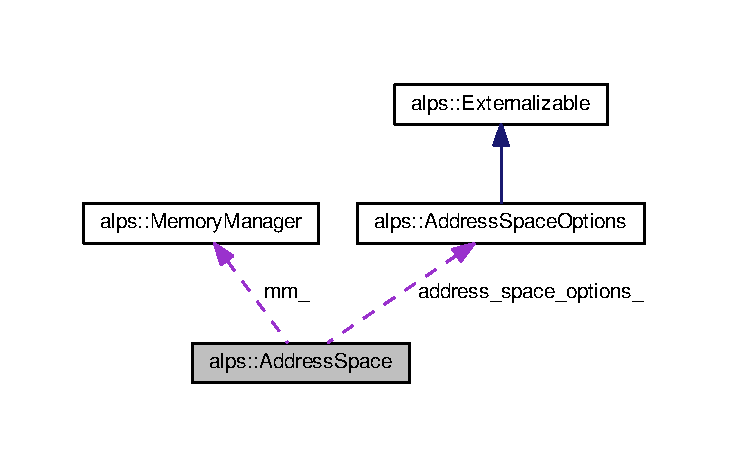
\includegraphics[width=350pt]{classalps_1_1AddressSpace__coll__graph}
\end{center}
\end{figure}
\subsection*{Public Member Functions}
\begin{DoxyCompactItemize}
\item 
{\bfseries Address\+Space} (const \hyperlink{structalps_1_1AddressSpaceOptions}{Address\+Space\+Options} \&address\+\_\+space\+\_\+options)\hypertarget{classalps_1_1AddressSpace_a4111cdf0156a0d6d0a865bef8d6a97b3}{}\label{classalps_1_1AddressSpace_a4111cdf0156a0d6d0a865bef8d6a97b3}

\item 
\hyperlink{group__ERRORCODES_ga6263a3c9a0b8d36aea21cdd835ac99fe}{Error\+Code} {\bfseries init} ()\hypertarget{classalps_1_1AddressSpace_aacc0bbb475a53159d582cb3c9a15109a}{}\label{classalps_1_1AddressSpace_aacc0bbb475a53159d582cb3c9a15109a}

\item 
{\footnotesize template$<$class RegionT $>$ }\\\hyperlink{group__ERRORCODES_ga6263a3c9a0b8d36aea21cdd835ac99fe}{Error\+Code} \hyperlink{classalps_1_1AddressSpace_a91628b6c9afb5796c4745d10d721c7df}{map} (\hyperlink{classalps_1_1RegionFile}{Region\+File} $\ast$region\+\_\+file, RegionT $\ast$$\ast$pregion)
\begin{DoxyCompactList}\small\item\em Maps a region file into the global address space. \end{DoxyCompactList}\item 
{\footnotesize template$<$class RegionT $>$ }\\\hyperlink{group__ERRORCODES_ga6263a3c9a0b8d36aea21cdd835ac99fe}{Error\+Code} \hyperlink{classalps_1_1AddressSpace_a94f33857ada089b1fb35bb7b3efc22f0}{bind} (RegionT $\ast$\hyperlink{classalps_1_1AddressSpace_a3f32659a01f535e8b787556c08270a68}{region}, Region\+Id region\+\_\+id)
\begin{DoxyCompactList}\small\item\em Binds a region to a shorthand name identifier. \end{DoxyCompactList}\item 
{\footnotesize template$<$class RegionT $>$ }\\\hyperlink{group__ERRORCODES_ga6263a3c9a0b8d36aea21cdd835ac99fe}{Error\+Code} \hyperlink{classalps_1_1AddressSpace_a23441f4279dbbf6f9d6fdb7da5c0626a}{unmap} (RegionT $\ast$\hyperlink{classalps_1_1AddressSpace_a3f32659a01f535e8b787556c08270a68}{region})
\begin{DoxyCompactList}\small\item\em Unmaps a previously mapped region. \end{DoxyCompactList}\item 
\hyperlink{classalps_1_1Region}{Region} $\ast$ \hyperlink{classalps_1_1AddressSpace_a3f32659a01f535e8b787556c08270a68}{region} (Region\+Id region\+\_\+id)
\begin{DoxyCompactList}\small\item\em Returns region identified by region identifier {\itshape region\+\_\+id}. \end{DoxyCompactList}\item 
\hyperlink{group__ERRORCODES_ga6263a3c9a0b8d36aea21cdd835ac99fe}{Error\+Code} \hyperlink{classalps_1_1AddressSpace_ae9c5ec2ca94b68aa80643676c3029de0}{rtrans} (void $\ast$vaddr, \hyperlink{classalps_1_1Region}{Region} $\ast$$\ast$pregion, Linear\+Addr $\ast$offset)
\begin{DoxyCompactList}\small\item\em Performs reverse translation of a virtual address to a $<${\itshape pregion}, {\itshape offset$>$} pair. \end{DoxyCompactList}\item 
\hyperlink{classalps_1_1MemoryManager}{Memory\+Manager} $\ast$ {\bfseries mm} ()\hypertarget{classalps_1_1AddressSpace_ac250b1b2b365f21f489a99e36122c679}{}\label{classalps_1_1AddressSpace_ac250b1b2b365f21f489a99e36122c679}

\end{DoxyCompactItemize}
\subsection*{Public Attributes}
\begin{DoxyCompactItemize}
\item 
\hyperlink{structalps_1_1AddressSpaceOptions}{Address\+Space\+Options} \hyperlink{classalps_1_1AddressSpace_ae41a0caf654a278553e05427538cd377}{address\+\_\+space\+\_\+options\+\_\+}\hypertarget{classalps_1_1AddressSpace_ae41a0caf654a278553e05427538cd377}{}\label{classalps_1_1AddressSpace_ae41a0caf654a278553e05427538cd377}

\begin{DoxyCompactList}\small\item\em Address space runtime options. \end{DoxyCompactList}\item 
\hyperlink{classalps_1_1MemoryManager}{Memory\+Manager} $\ast$ \hyperlink{classalps_1_1AddressSpace_ab4e162ae17ddc0c15873e910c075169d}{mm\+\_\+}\hypertarget{classalps_1_1AddressSpace_ab4e162ae17ddc0c15873e910c075169d}{}\label{classalps_1_1AddressSpace_ab4e162ae17ddc0c15873e910c075169d}

\begin{DoxyCompactList}\small\item\em Memory manager mapping regions into virtual memory. \end{DoxyCompactList}\item 
std\+::multimap$<$ Region\+Id, \hyperlink{classalps_1_1Region}{Region} $\ast$ $>$ \hyperlink{classalps_1_1AddressSpace_a6cba6ed6bb0ffee7682fc665b4eaa035}{regions\+\_\+}\hypertarget{classalps_1_1AddressSpace_a6cba6ed6bb0ffee7682fc665b4eaa035}{}\label{classalps_1_1AddressSpace_a6cba6ed6bb0ffee7682fc665b4eaa035}

\begin{DoxyCompactList}\small\item\em A table mapping region\+\_\+id to region. \end{DoxyCompactList}\end{DoxyCompactItemize}


\subsection{Detailed Description}
Represents a logical address space where region files can be bound and mapped to. There should be a single \hyperlink{classalps_1_1AddressSpace}{Address\+Space} object instance per process even though nothing prevents a user from having multiple instances.

Mapping and binding a region file to a global address space results in a named region. The global address space supports different modes of region mappings to allow users select different performance and flexibility tradeoffs. These modes are supported through template polymorphism rather than virtual polymorphish to reduce the runtime overhead for accessing regions.

Mapping modes include\+:
\begin{DoxyItemize}
\item single segment direct relocatable mapping, where the whole region is directly mapped to an arbitraty address. This mode enables using relative offset pointers (similar to offset\+\_\+ptr) for flexible mapping and addressing at the expense of performance (i.\+e., some overhead to perform simple pointer arithmetic relative to the base of region). 
\end{DoxyItemize}

\subsection{Member Function Documentation}
\index{alps\+::\+Address\+Space@{alps\+::\+Address\+Space}!bind@{bind}}
\index{bind@{bind}!alps\+::\+Address\+Space@{alps\+::\+Address\+Space}}
\subsubsection[{\texorpdfstring{bind(\+Region\+T $\ast$region, Region\+Id region\+\_\+id)}{bind(RegionT *region, RegionId region_id)}}]{\setlength{\rightskip}{0pt plus 5cm}template$<$class RegionT $>$ {\bf Error\+Code} alps\+::\+Address\+Space\+::bind (
\begin{DoxyParamCaption}
\item[{RegionT $\ast$}]{region, }
\item[{Region\+Id}]{region\+\_\+id}
\end{DoxyParamCaption}
)}\hypertarget{classalps_1_1AddressSpace_a94f33857ada089b1fb35bb7b3efc22f0}{}\label{classalps_1_1AddressSpace_a94f33857ada089b1fb35bb7b3efc22f0}

\begin{DoxyParams}[1]{Parameters}
\mbox{\tt in}  & {\em region} & The region object to bind. \\
\hline
\mbox{\tt in}  & {\em region\+\_\+id} & The shorthand name identifier to bind the region to.\\
\hline
\end{DoxyParams}
After binding, pointers can identify the region using the shorthand name identifier. \index{alps\+::\+Address\+Space@{alps\+::\+Address\+Space}!map@{map}}
\index{map@{map}!alps\+::\+Address\+Space@{alps\+::\+Address\+Space}}
\subsubsection[{\texorpdfstring{map(\+Region\+File $\ast$region\+\_\+file, Region\+T $\ast$$\ast$pregion)}{map(RegionFile *region_file, RegionT **pregion)}}]{\setlength{\rightskip}{0pt plus 5cm}template$<$class RegionT $>$ template {\bf Error\+Code} alps\+::\+Address\+Space\+::map$<$ {\bf R\+Region} $>$ (
\begin{DoxyParamCaption}
\item[{{\bf Region\+File} $\ast$}]{region\+\_\+file, }
\item[{RegionT $\ast$$\ast$}]{pregion}
\end{DoxyParamCaption}
)}\hypertarget{classalps_1_1AddressSpace_a91628b6c9afb5796c4745d10d721c7df}{}\label{classalps_1_1AddressSpace_a91628b6c9afb5796c4745d10d721c7df}

\begin{DoxyParams}[1]{Parameters}
\mbox{\tt in}  & {\em region\+\_\+file} & The region file to map into the global address space. \\
\hline
\mbox{\tt out}  & {\em pregion} & An object representing the region of the global address space where the file is mapped to. \\
\hline
\end{DoxyParams}
\index{alps\+::\+Address\+Space@{alps\+::\+Address\+Space}!region@{region}}
\index{region@{region}!alps\+::\+Address\+Space@{alps\+::\+Address\+Space}}
\subsubsection[{\texorpdfstring{region(\+Region\+Id region\+\_\+id)}{region(RegionId region_id)}}]{\setlength{\rightskip}{0pt plus 5cm}{\bf Region} $\ast$ alps\+::\+Address\+Space\+::region (
\begin{DoxyParamCaption}
\item[{Region\+Id}]{region\+\_\+id}
\end{DoxyParamCaption}
)}\hypertarget{classalps_1_1AddressSpace_a3f32659a01f535e8b787556c08270a68}{}\label{classalps_1_1AddressSpace_a3f32659a01f535e8b787556c08270a68}

\begin{DoxyParams}[1]{Parameters}
\mbox{\tt in}  & {\em region\+\_\+id} & \hyperlink{classalps_1_1Region}{Region} identifier \\
\hline
\end{DoxyParams}
\index{alps\+::\+Address\+Space@{alps\+::\+Address\+Space}!rtrans@{rtrans}}
\index{rtrans@{rtrans}!alps\+::\+Address\+Space@{alps\+::\+Address\+Space}}
\subsubsection[{\texorpdfstring{rtrans(void $\ast$vaddr, Region $\ast$$\ast$pregion, Linear\+Addr $\ast$offset)}{rtrans(void *vaddr, Region **pregion, LinearAddr *offset)}}]{\setlength{\rightskip}{0pt plus 5cm}{\bf Error\+Code} alps\+::\+Address\+Space\+::rtrans (
\begin{DoxyParamCaption}
\item[{void $\ast$}]{vaddr, }
\item[{{\bf Region} $\ast$$\ast$}]{pregion, }
\item[{Linear\+Addr $\ast$}]{offset}
\end{DoxyParamCaption}
)}\hypertarget{classalps_1_1AddressSpace_ae9c5ec2ca94b68aa80643676c3029de0}{}\label{classalps_1_1AddressSpace_ae9c5ec2ca94b68aa80643676c3029de0}

\begin{DoxyParams}[1]{Parameters}
\mbox{\tt in}  & {\em vaddr} & The virtual address to reverse translate. \\
\hline
\mbox{\tt out}  & {\em pregion} & The region the virtual address is mapped to. \\
\hline
\mbox{\tt out}  & {\em offset} & The offset relative to the region base. \\
\hline
\end{DoxyParams}
\index{alps\+::\+Address\+Space@{alps\+::\+Address\+Space}!unmap@{unmap}}
\index{unmap@{unmap}!alps\+::\+Address\+Space@{alps\+::\+Address\+Space}}
\subsubsection[{\texorpdfstring{unmap(\+Region\+T $\ast$region)}{unmap(RegionT *region)}}]{\setlength{\rightskip}{0pt plus 5cm}template$<$class RegionT $>$ template {\bf Error\+Code} alps\+::\+Address\+Space\+::unmap$<$ {\bf R\+Region} $>$ (
\begin{DoxyParamCaption}
\item[{RegionT $\ast$}]{region}
\end{DoxyParamCaption}
)}\hypertarget{classalps_1_1AddressSpace_a23441f4279dbbf6f9d6fdb7da5c0626a}{}\label{classalps_1_1AddressSpace_a23441f4279dbbf6f9d6fdb7da5c0626a}

\begin{DoxyParams}[1]{Parameters}
\mbox{\tt in}  & {\em region} & The region object to unmap. \\
\hline
\end{DoxyParams}


The documentation for this class was generated from the following files\+:\begin{DoxyCompactItemize}
\item 
/home/yuan/\+Benchmarks/whisper/mnemosyne-\/gcc/usermode/library/pmalloc/include/alps/include/alps/pegasus/address\+\_\+space.\+hh\item 
/home/yuan/\+Benchmarks/whisper/mnemosyne-\/gcc/usermode/library/pmalloc/include/alps/src/pegasus/address\+\_\+space.\+cc\end{DoxyCompactItemize}

\hypertarget{structalps_1_1AddressSpaceOptions}{}\section{alps\+:\+:Address\+Space\+Options Struct Reference}
\label{structalps_1_1AddressSpaceOptions}\index{alps\+::\+Address\+Space\+Options@{alps\+::\+Address\+Space\+Options}}


Inheritance diagram for alps\+:\+:Address\+Space\+Options\+:
\nopagebreak
\begin{figure}[H]
\begin{center}
\leavevmode
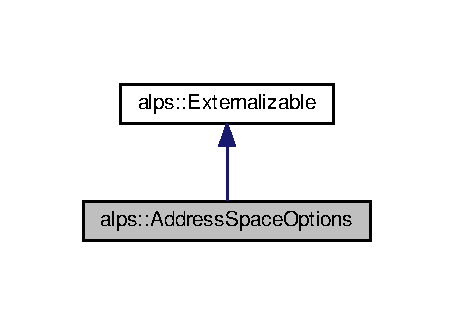
\includegraphics[width=218pt]{structalps_1_1AddressSpaceOptions__inherit__graph}
\end{center}
\end{figure}


Collaboration diagram for alps\+:\+:Address\+Space\+Options\+:
\nopagebreak
\begin{figure}[H]
\begin{center}
\leavevmode
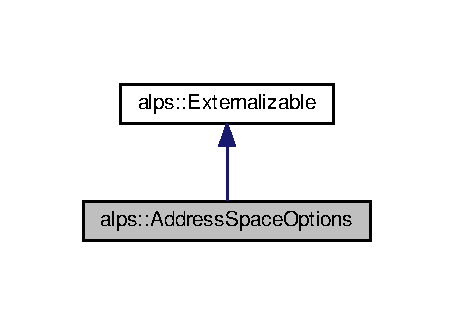
\includegraphics[width=218pt]{structalps_1_1AddressSpaceOptions__coll__graph}
\end{center}
\end{figure}
\subsection*{Public Member Functions}
\begin{DoxyCompactItemize}
\item 
\hyperlink{structalps_1_1AddressSpaceOptions_a6e0027f273736238952ad058a3650c54}{Address\+Space\+Options} ()
\end{DoxyCompactItemize}
\subsection*{Public Attributes}
\begin{DoxyCompactItemize}
\item 
bool {\bfseries k\+Default\+Allow\+Duplicate\+Mappings} = false\hypertarget{structalps_1_1AddressSpaceOptions_a5b9adf6f093ea3188c6b267cf0328488}{}\label{structalps_1_1AddressSpaceOptions_a5b9adf6f093ea3188c6b267cf0328488}

\item 
uint64\+\_\+t {\bfseries allow\+\_\+duplicate\+\_\+mappings}\hypertarget{structalps_1_1AddressSpaceOptions_a3004311f8e4eede84c6bbd98fabe2312}{}\label{structalps_1_1AddressSpaceOptions_a3004311f8e4eede84c6bbd98fabe2312}

\end{DoxyCompactItemize}
\subsection*{Additional Inherited Members}


\subsection{Constructor \& Destructor Documentation}
\index{alps\+::\+Address\+Space\+Options@{alps\+::\+Address\+Space\+Options}!Address\+Space\+Options@{Address\+Space\+Options}}
\index{Address\+Space\+Options@{Address\+Space\+Options}!alps\+::\+Address\+Space\+Options@{alps\+::\+Address\+Space\+Options}}
\subsubsection[{\texorpdfstring{Address\+Space\+Options()}{AddressSpaceOptions()}}]{\setlength{\rightskip}{0pt plus 5cm}alps\+::\+Address\+Space\+Options\+::\+Address\+Space\+Options (
\begin{DoxyParamCaption}
{}
\end{DoxyParamCaption}
)\hspace{0.3cm}{\ttfamily [inline]}}\hypertarget{structalps_1_1AddressSpaceOptions_a6e0027f273736238952ad058a3650c54}{}\label{structalps_1_1AddressSpaceOptions_a6e0027f273736238952ad058a3650c54}
Constructs option values with default values 

The documentation for this struct was generated from the following file\+:\begin{DoxyCompactItemize}
\item 
/home/yuan/\+Benchmarks/whisper/mnemosyne-\/gcc/usermode/library/pmalloc/include/alps/include/alps/pegasus/address\+\_\+space\+\_\+options.\+hh\end{DoxyCompactItemize}

\hypertarget{structalps_1_1BacktraceContext}{}\section{alps\+:\+:Backtrace\+Context Struct Reference}
\label{structalps_1_1BacktraceContext}\index{alps\+::\+Backtrace\+Context@{alps\+::\+Backtrace\+Context}}
\subsection*{Classes}
\begin{DoxyCompactItemize}
\item 
struct \hyperlink{structalps_1_1BacktraceContext_1_1GlibcBacktraceInfo}{Glibc\+Backtrace\+Info}
\item 
struct \hyperlink{structalps_1_1BacktraceContext_1_1LibBacktraceInfo}{Lib\+Backtrace\+Info}
\end{DoxyCompactItemize}
\subsection*{Public Types}
\begin{DoxyCompactItemize}
\item 
enum {\bfseries Constants} \{ {\bfseries k\+Max\+Depth} = 64
 \}\hypertarget{structalps_1_1BacktraceContext_ab3446800cb2eb7430805f58d18b5f5e8}{}\label{structalps_1_1BacktraceContext_ab3446800cb2eb7430805f58d18b5f5e8}

\end{DoxyCompactItemize}
\subsection*{Public Member Functions}
\begin{DoxyCompactItemize}
\item 
void {\bfseries release} ()\hypertarget{structalps_1_1BacktraceContext_a937b2b9142142e160635cc13936f896c}{}\label{structalps_1_1BacktraceContext_a937b2b9142142e160635cc13936f896c}

\item 
void {\bfseries call\+\_\+glibc\+\_\+backtrace} ()\hypertarget{structalps_1_1BacktraceContext_a42c19d83492f8ff5901f97b71790af57}{}\label{structalps_1_1BacktraceContext_a42c19d83492f8ff5901f97b71790af57}

\item 
void {\bfseries on\+\_\+libbt\+\_\+create\+\_\+state\+\_\+error} (const char $\ast$msg, int errnum)\hypertarget{structalps_1_1BacktraceContext_a2dfa89eef1db391b241659d852e90bba}{}\label{structalps_1_1BacktraceContext_a2dfa89eef1db391b241659d852e90bba}

\item 
void {\bfseries on\+\_\+libbt\+\_\+full\+\_\+error} (const char $\ast$msg, int errnum)\hypertarget{structalps_1_1BacktraceContext_a008aed155d81d3e65d46543c72363470}{}\label{structalps_1_1BacktraceContext_a008aed155d81d3e65d46543c72363470}

\item 
void {\bfseries on\+\_\+libbt\+\_\+full} (uintptr\+\_\+t pc, const char $\ast$filename, int lineno, const char $\ast$function)\hypertarget{structalps_1_1BacktraceContext_a0adf3b6e197546585be28575dfc445f1}{}\label{structalps_1_1BacktraceContext_a0adf3b6e197546585be28575dfc445f1}

\item 
std\+::vector$<$ std\+::string $>$ {\bfseries get\+\_\+results} (uint16\+\_\+t skip)\hypertarget{structalps_1_1BacktraceContext_a44d0d8ee89d984f60e6c35f18689a502}{}\label{structalps_1_1BacktraceContext_a44d0d8ee89d984f60e6c35f18689a502}

\end{DoxyCompactItemize}
\subsection*{Public Attributes}
\begin{DoxyCompactItemize}
\item 
std\+::string {\bfseries error\+\_\+}\hypertarget{structalps_1_1BacktraceContext_a07243a40f28635c9fd8a7142458f5d03}{}\label{structalps_1_1BacktraceContext_a07243a40f28635c9fd8a7142458f5d03}

\item 
std\+::vector$<$ \hyperlink{structalps_1_1BacktraceContext_1_1GlibcBacktraceInfo}{Glibc\+Backtrace\+Info} $>$ {\bfseries glibc\+\_\+bt\+\_\+info\+\_\+}\hypertarget{structalps_1_1BacktraceContext_a6209c0529da5d3ee7a9ffc15cd68cfdc}{}\label{structalps_1_1BacktraceContext_a6209c0529da5d3ee7a9ffc15cd68cfdc}

\item 
std\+::vector$<$ \hyperlink{structalps_1_1BacktraceContext_1_1LibBacktraceInfo}{Lib\+Backtrace\+Info} $>$ {\bfseries libbt\+\_\+info\+\_\+}\hypertarget{structalps_1_1BacktraceContext_a4b87abda6b6d9f3ce5e6096269a61500}{}\label{structalps_1_1BacktraceContext_a4b87abda6b6d9f3ce5e6096269a61500}

\end{DoxyCompactItemize}


The documentation for this struct was generated from the following file\+:\begin{DoxyCompactItemize}
\item 
/home/yuan/\+Benchmarks/whisper/mnemosyne-\/gcc/usermode/library/pmalloc/include/alps/src/common/rich\+\_\+backtrace.\+cc\end{DoxyCompactItemize}

\hypertarget{classalps_1_1BaseRelativePointer}{}\section{alps\+:\+:Base\+Relative\+Pointer Class Reference}
\label{classalps_1_1BaseRelativePointer}\index{alps\+::\+Base\+Relative\+Pointer@{alps\+::\+Base\+Relative\+Pointer}}
\subsection*{Classes}
\begin{DoxyCompactItemize}
\item 
class \hyperlink{classalps_1_1BaseRelativePointer_1_1IPtr}{I\+Ptr}
\begin{DoxyCompactList}\small\item\em Intermediate representation of a relocatable pointer. \end{DoxyCompactList}\item 
class \hyperlink{classalps_1_1BaseRelativePointer_1_1PPtr}{P\+Ptr}
\begin{DoxyCompactList}\small\item\em Represents a linear persistent pointer. \end{DoxyCompactList}\item 
class \hyperlink{classalps_1_1BaseRelativePointer_1_1TPtr}{T\+Ptr}
\begin{DoxyCompactList}\small\item\em Represents a transient pointer. \end{DoxyCompactList}\item 
class \hyperlink{classalps_1_1BaseRelativePointer_1_1ZPtr}{Z\+Ptr}
\end{DoxyCompactItemize}


The documentation for this class was generated from the following file\+:\begin{DoxyCompactItemize}
\item 
/home/yuan/\+Benchmarks/whisper/mnemosyne-\/gcc/usermode/library/pmalloc/include/alps/include/alps/pegasus/pointer.\+hh\end{DoxyCompactItemize}

\hypertarget{structalps_1_1CommandOption}{}\section{alps\+:\+:Command\+Option Struct Reference}
\label{structalps_1_1CommandOption}\index{alps\+::\+Command\+Option@{alps\+::\+Command\+Option}}


Inheritance diagram for alps\+:\+:Command\+Option\+:
\nopagebreak
\begin{figure}[H]
\begin{center}
\leavevmode
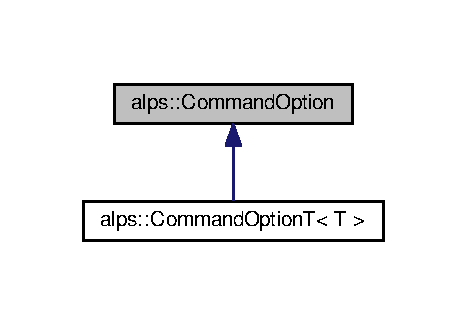
\includegraphics[width=224pt]{structalps_1_1CommandOption__inherit__graph}
\end{center}
\end{figure}
\subsection*{Public Member Functions}
\begin{DoxyCompactItemize}
\item 
virtual void {\bfseries add\+\_\+option} (boost\+::program\+\_\+options\+::options\+\_\+description \&desc)=0\hypertarget{structalps_1_1CommandOption_a8c092a8a61f3d12081702ab1fcc6bc06}{}\label{structalps_1_1CommandOption_a8c092a8a61f3d12081702ab1fcc6bc06}

\item 
virtual std\+::string {\bfseries argname} ()=0\hypertarget{structalps_1_1CommandOption_a8315b5ecacc49493f4c9eb9106ae0265}{}\label{structalps_1_1CommandOption_a8315b5ecacc49493f4c9eb9106ae0265}

\item 
virtual void {\bfseries set\+\_\+value} (const boost\+::program\+\_\+options\+::variable\+\_\+value \&val)=0\hypertarget{structalps_1_1CommandOption_abc7792c9b9c2d85ed64e9ebf45e680f0}{}\label{structalps_1_1CommandOption_abc7792c9b9c2d85ed64e9ebf45e680f0}

\end{DoxyCompactItemize}


The documentation for this struct was generated from the following file\+:\begin{DoxyCompactItemize}
\item 
/home/yuan/\+Benchmarks/whisper/mnemosyne-\/gcc/usermode/library/pmalloc/include/alps/include/alps/common/externalizable.\+hh\end{DoxyCompactItemize}

\hypertarget{structalps_1_1CommandOptionT}{}\section{alps\+:\+:Command\+OptionT$<$ T $>$ Struct Template Reference}
\label{structalps_1_1CommandOptionT}\index{alps\+::\+Command\+Option\+T$<$ T $>$@{alps\+::\+Command\+Option\+T$<$ T $>$}}


Inheritance diagram for alps\+:\+:Command\+OptionT$<$ T $>$\+:
\nopagebreak
\begin{figure}[H]
\begin{center}
\leavevmode
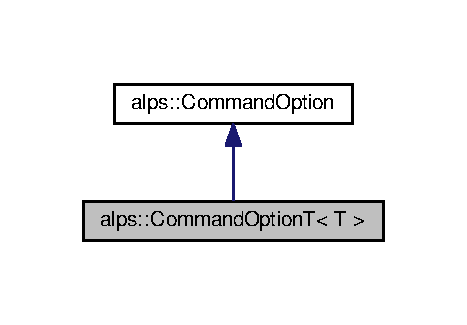
\includegraphics[width=224pt]{structalps_1_1CommandOptionT__inherit__graph}
\end{center}
\end{figure}


Collaboration diagram for alps\+:\+:Command\+OptionT$<$ T $>$\+:
\nopagebreak
\begin{figure}[H]
\begin{center}
\leavevmode
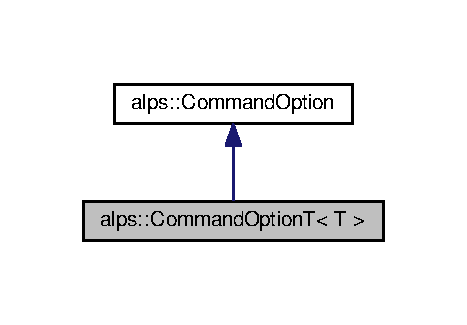
\includegraphics[width=224pt]{structalps_1_1CommandOptionT__coll__graph}
\end{center}
\end{figure}
\subsection*{Public Member Functions}
\begin{DoxyCompactItemize}
\item 
{\bfseries Command\+OptionT} (std\+::string argname, T $\ast$out, std\+::string desc)\hypertarget{structalps_1_1CommandOptionT_afeb7017b64f54b68d780ff44a669bb4b}{}\label{structalps_1_1CommandOptionT_afeb7017b64f54b68d780ff44a669bb4b}

\item 
std\+::string {\bfseries argname} ()\hypertarget{structalps_1_1CommandOptionT_adc65402419f6cb0161a027093b17f6c3}{}\label{structalps_1_1CommandOptionT_adc65402419f6cb0161a027093b17f6c3}

\item 
void {\bfseries add\+\_\+option} (boost\+::program\+\_\+options\+::options\+\_\+description \&desc)\hypertarget{structalps_1_1CommandOptionT_a960f8fc45f3f61b5769de59c955e2ab8}{}\label{structalps_1_1CommandOptionT_a960f8fc45f3f61b5769de59c955e2ab8}

\item 
void {\bfseries set\+\_\+value} (const boost\+::program\+\_\+options\+::variable\+\_\+value \&val)\hypertarget{structalps_1_1CommandOptionT_a05e50058ec74d24f799a7cfe311b39f0}{}\label{structalps_1_1CommandOptionT_a05e50058ec74d24f799a7cfe311b39f0}

\end{DoxyCompactItemize}
\subsection*{Public Attributes}
\begin{DoxyCompactItemize}
\item 
std\+::string {\bfseries argname\+\_\+}\hypertarget{structalps_1_1CommandOptionT_ae81a9788b7a13e96549630200234e1fe}{}\label{structalps_1_1CommandOptionT_ae81a9788b7a13e96549630200234e1fe}

\item 
T $\ast$ {\bfseries out\+\_\+}\hypertarget{structalps_1_1CommandOptionT_acb37d7fc0de3c05d142ca94b6284f368}{}\label{structalps_1_1CommandOptionT_acb37d7fc0de3c05d142ca94b6284f368}

\item 
std\+::string {\bfseries desc\+\_\+}\hypertarget{structalps_1_1CommandOptionT_a61c2aa354e9e80303f05f1c59172f9d6}{}\label{structalps_1_1CommandOptionT_a61c2aa354e9e80303f05f1c59172f9d6}

\end{DoxyCompactItemize}


The documentation for this struct was generated from the following file\+:\begin{DoxyCompactItemize}
\item 
/home/yuan/\+Benchmarks/whisper/mnemosyne-\/gcc/usermode/library/pmalloc/include/alps/include/alps/common/externalizable.\+hh\end{DoxyCompactItemize}

\hypertarget{structalps_1_1DebugOptions}{}\section{alps\+:\+:Debug\+Options Struct Reference}
\label{structalps_1_1DebugOptions}\index{alps\+::\+Debug\+Options@{alps\+::\+Debug\+Options}}


Inheritance diagram for alps\+:\+:Debug\+Options\+:
\nopagebreak
\begin{figure}[H]
\begin{center}
\leavevmode
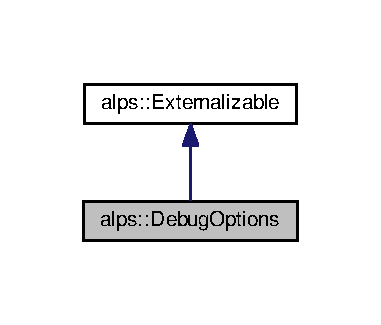
\includegraphics[width=183pt]{structalps_1_1DebugOptions__inherit__graph}
\end{center}
\end{figure}


Collaboration diagram for alps\+:\+:Debug\+Options\+:
\nopagebreak
\begin{figure}[H]
\begin{center}
\leavevmode
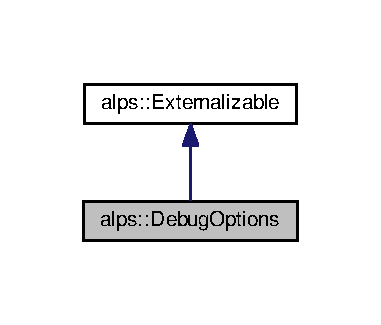
\includegraphics[width=183pt]{structalps_1_1DebugOptions__coll__graph}
\end{center}
\end{figure}
\subsection*{Public Member Functions}
\begin{DoxyCompactItemize}
\item 
\hyperlink{structalps_1_1DebugOptions_ac80b967acde2e4b8bf67efea07c2daff}{Debug\+Options} ()
\end{DoxyCompactItemize}
\subsection*{Public Attributes}
\begin{DoxyCompactItemize}
\item 
std\+::string {\bfseries k\+Default\+Log\+Filename} = \char`\"{}sample.\+log\char`\"{}\hypertarget{structalps_1_1DebugOptions_af2279520d557f5910f55f2f755b64b67}{}\label{structalps_1_1DebugOptions_af2279520d557f5910f55f2f755b64b67}

\item 
std\+::string {\bfseries k\+Default\+Log\+Level} = \char`\"{}error\char`\"{}\hypertarget{structalps_1_1DebugOptions_a8c5210aee621db376d6eca159a2cdb15}{}\label{structalps_1_1DebugOptions_a8c5210aee621db376d6eca159a2cdb15}

\item 
std\+::string \hyperlink{structalps_1_1DebugOptions_a777ede2e77a0fed168bdcfe8ebe19465}{log\+\_\+filename}
\item 
std\+::string \hyperlink{structalps_1_1DebugOptions_a6c5c875c884d1580128aa0c095dcf5dd}{log\+\_\+level}
\end{DoxyCompactItemize}
\subsection*{Additional Inherited Members}


\subsection{Constructor \& Destructor Documentation}
\index{alps\+::\+Debug\+Options@{alps\+::\+Debug\+Options}!Debug\+Options@{Debug\+Options}}
\index{Debug\+Options@{Debug\+Options}!alps\+::\+Debug\+Options@{alps\+::\+Debug\+Options}}
\subsubsection[{\texorpdfstring{Debug\+Options()}{DebugOptions()}}]{\setlength{\rightskip}{0pt plus 5cm}alps\+::\+Debug\+Options\+::\+Debug\+Options (
\begin{DoxyParamCaption}
{}
\end{DoxyParamCaption}
)\hspace{0.3cm}{\ttfamily [inline]}}\hypertarget{structalps_1_1DebugOptions_ac80b967acde2e4b8bf67efea07c2daff}{}\label{structalps_1_1DebugOptions_ac80b967acde2e4b8bf67efea07c2daff}
Constructs option values with default values 

\subsection{Member Data Documentation}
\index{alps\+::\+Debug\+Options@{alps\+::\+Debug\+Options}!log\+\_\+filename@{log\+\_\+filename}}
\index{log\+\_\+filename@{log\+\_\+filename}!alps\+::\+Debug\+Options@{alps\+::\+Debug\+Options}}
\subsubsection[{\texorpdfstring{log\+\_\+filename}{log_filename}}]{\setlength{\rightskip}{0pt plus 5cm}std\+::string alps\+::\+Debug\+Options\+::log\+\_\+filename}\hypertarget{structalps_1_1DebugOptions_a777ede2e77a0fed168bdcfe8ebe19465}{}\label{structalps_1_1DebugOptions_a777ede2e77a0fed168bdcfe8ebe19465}
Store log messages to this file \index{alps\+::\+Debug\+Options@{alps\+::\+Debug\+Options}!log\+\_\+level@{log\+\_\+level}}
\index{log\+\_\+level@{log\+\_\+level}!alps\+::\+Debug\+Options@{alps\+::\+Debug\+Options}}
\subsubsection[{\texorpdfstring{log\+\_\+level}{log_level}}]{\setlength{\rightskip}{0pt plus 5cm}std\+::string alps\+::\+Debug\+Options\+::log\+\_\+level}\hypertarget{structalps_1_1DebugOptions_a6c5c875c884d1580128aa0c095dcf5dd}{}\label{structalps_1_1DebugOptions_a6c5c875c884d1580128aa0c095dcf5dd}
Log messages at or above this level 

The documentation for this struct was generated from the following file\+:\begin{DoxyCompactItemize}
\item 
/home/yuan/\+Benchmarks/whisper/mnemosyne-\/gcc/usermode/library/pmalloc/include/alps/include/alps/common/debug\+\_\+options.\+hh\end{DoxyCompactItemize}

\hypertarget{classalps_1_1ErrorStack}{}\section{alps\+:\+:Error\+Stack Class Reference}
\label{classalps_1_1ErrorStack}\index{alps\+::\+Error\+Stack@{alps\+::\+Error\+Stack}}


Brings error stacktrace information as return value of functions.  




{\ttfamily \#include $<$error\+\_\+stack.\+hh$>$}

\subsection*{Public Types}
\begin{DoxyCompactItemize}
\item 
enum \hyperlink{classalps_1_1ErrorStack_a18b861743a2de89ca205ffa2d91e6997}{Constants} \{ \hyperlink{classalps_1_1ErrorStack_a18b861743a2de89ca205ffa2d91e6997abd01de12344bb39aa89faef49805ac46}{k\+Max\+Stack\+Depth} = 8
 \}
\end{DoxyCompactItemize}
\subsection*{Public Member Functions}
\begin{DoxyCompactItemize}
\item 
\hyperlink{classalps_1_1ErrorStack_af45fef4cca00ffee757cc9cc3785a0a8}{Error\+Stack} ()
\item 
\hyperlink{classalps_1_1ErrorStack_ad40706ec9b58151b37fda5096f77b718}{Error\+Stack} (\hyperlink{group__ERRORCODES_ga6263a3c9a0b8d36aea21cdd835ac99fe}{Error\+Code} code)
\begin{DoxyCompactList}\small\item\em Instantiate a return code without a custom error message nor stacktrace. \end{DoxyCompactList}\item 
\hyperlink{classalps_1_1ErrorStack_aaee609e98f03c2733af1203036e3f6e0}{Error\+Stack} (const char $\ast$filename, const char $\ast$func, uint32\+\_\+t linenum, \hyperlink{group__ERRORCODES_ga6263a3c9a0b8d36aea21cdd835ac99fe}{Error\+Code} code, const char $\ast$custom\+\_\+message=\hyperlink{group__CXX11_ga213f92e16813051c59cdccf6d28baa78}{C\+X\+X11\+\_\+\+N\+U\+L\+L\+P\+TR})
\begin{DoxyCompactList}\small\item\em Instantiate a return code with stacktrace and optionally a custom error message. \end{DoxyCompactList}\item 
\hyperlink{classalps_1_1ErrorStack_a9222f3cb9055701981493a1451b321e4}{Error\+Stack} (const \hyperlink{classalps_1_1ErrorStack}{Error\+Stack} \&other)
\item 
\hyperlink{classalps_1_1ErrorStack_a5e43623d23880edd151f921dec114a5d}{Error\+Stack} (const \hyperlink{classalps_1_1ErrorStack}{Error\+Stack} \&other, const char $\ast$filename, const char $\ast$func, uint32\+\_\+t linenum, const char $\ast$more\+\_\+custom\+\_\+message=\hyperlink{group__CXX11_ga213f92e16813051c59cdccf6d28baa78}{C\+X\+X11\+\_\+\+N\+U\+L\+L\+P\+TR})
\item 
\hyperlink{classalps_1_1ErrorStack}{Error\+Stack} \& \hyperlink{classalps_1_1ErrorStack_a9719a01f9e25cd67bbd632521524e888}{operator=} (const \hyperlink{classalps_1_1ErrorStack}{Error\+Stack} \&other)
\item 
\hyperlink{classalps_1_1ErrorStack_afb344b60c5d325aebbd6b9b278357df2}{$\sim$\+Error\+Stack} ()
\item 
bool \hyperlink{classalps_1_1ErrorStack_a6a1333e8b975b92de8628e8b3c5058dc}{is\+\_\+error} () const 
\item 
\hyperlink{group__ERRORCODES_ga6263a3c9a0b8d36aea21cdd835ac99fe}{Error\+Code} \hyperlink{classalps_1_1ErrorStack_acad692aa115b80ee36ad173c5aa9e2eb}{get\+\_\+error\+\_\+code} () const 
\item 
const char $\ast$ \hyperlink{classalps_1_1ErrorStack_ad6d3e825281c3bc8ed7aee7ba0a35b74}{get\+\_\+message} () const 
\item 
const char $\ast$ \hyperlink{classalps_1_1ErrorStack_aa5814d07d45601b0f54b77c2b456ba8c}{get\+\_\+custom\+\_\+message} () const 
\item 
void \hyperlink{classalps_1_1ErrorStack_a68a61726008208d49521db039a18d2d9}{copy\+\_\+custom\+\_\+message} (const char $\ast$message)
\item 
void \hyperlink{classalps_1_1ErrorStack_a416b4574f9f73063720cb20c620dad51}{clear\+\_\+custom\+\_\+message} ()
\item 
void \hyperlink{classalps_1_1ErrorStack_ae89827aafd6095698f9b223ebecea40b}{append\+\_\+custom\+\_\+message} (const char $\ast$more\+\_\+custom\+\_\+message)
\item 
uint16\+\_\+t \hyperlink{classalps_1_1ErrorStack_aeb0920c79b84e369eecd694cc8261ff1}{get\+\_\+stack\+\_\+depth} () const 
\item 
uint32\+\_\+t \hyperlink{classalps_1_1ErrorStack_ae4b6ae74770f2f45e9f6161785c05b2b}{get\+\_\+linenum} (uint16\+\_\+t stack\+\_\+index) const 
\item 
const char $\ast$ \hyperlink{classalps_1_1ErrorStack_ad13251b97c0b40b0901f606f9d6d5384}{get\+\_\+filename} (uint16\+\_\+t stack\+\_\+index) const 
\item 
const char $\ast$ \hyperlink{classalps_1_1ErrorStack_a738f149173bc7e9a7be827dd7a02de8f}{get\+\_\+func} (uint16\+\_\+t stack\+\_\+index) const 
\item 
int \hyperlink{classalps_1_1ErrorStack_a1d7e8a20295213f32de56a5b77b976c1}{get\+\_\+os\+\_\+errno} () const 
\item 
void \hyperlink{classalps_1_1ErrorStack_ad157dbc40b5c2eaccd44dd7347296a45}{verify} () const 
\item 
void \hyperlink{classalps_1_1ErrorStack_afe67ad7f9830b1ef263f867109230b54}{output} (std\+::ostream $\ast$ptr) const 
\item 
void \hyperlink{classalps_1_1ErrorStack_a30461e6b34692f7ee11db1995d52d0ac}{dump\+\_\+and\+\_\+abort} (const char $\ast$abort\+\_\+message) const 
\end{DoxyCompactItemize}
\subsection*{Static Public Member Functions}
\begin{DoxyCompactItemize}
\item 
static std\+::string \hyperlink{classalps_1_1ErrorStack_a4e7dfdf688e6a33bbda2cfebf3a396a7}{get\+\_\+recent\+\_\+dump\+\_\+and\+\_\+abort} ()
\end{DoxyCompactItemize}
\subsection*{Friends}
\begin{DoxyCompactItemize}
\item 
std\+::ostream \& {\bfseries operator$<$$<$} (std\+::ostream \&o, const \hyperlink{classalps_1_1ErrorStack}{Error\+Stack} \&obj)\hypertarget{classalps_1_1ErrorStack_adfc96f96e5d8f4c12b4a9cea60c1fbb4}{}\label{classalps_1_1ErrorStack_adfc96f96e5d8f4c12b4a9cea60c1fbb4}

\end{DoxyCompactItemize}


\subsection{Detailed Description}
This is returned by many A\+PI functions. As it brings stacktrace information, it\textquotesingle{}s more informative than just returning Error\+Code. However, note that instantiating and augmenting this stack object has some overhead.

\begin{DoxyParagraph}{Why not exception}
A couple of reasons\+: \begin{DoxyItemize}
\item Performance \item Portability \item Our Google C++ Coding Style overlord said so\end{DoxyItemize}
We are not even sure what exceptions would look like in future environments. So, we don\textquotesingle{}t throw or catch any exceptions in our program.
\end{DoxyParagraph}
\begin{DoxyParagraph}{Macros to help use Error\+Stack}
In most places, you should use k\+Ret\+Ok, \hyperlink{group__ERRORCODES_ga72a80915c3588aea09c053ab567e19c4}{C\+H\+E\+C\+K\+\_\+\+E\+R\+R\+O\+R(x)}, or \hyperlink{group__ERRORCODES_gaf2fc6952d71aa10a52c326a27a0746da}{E\+R\+R\+O\+R\+\_\+\+S\+T\+A\+C\+K(e)} to handle this class. See the doucments of those macros.
\end{DoxyParagraph}
\begin{DoxyParagraph}{Forced return code checking}
An error code must be checked by some code, else it will abort with an \char`\"{}error-\/not-\/checked\char`\"{} error in stderr. We might later make this warning instead of aborting, but we should keep the current setting for a while to check for undesired coding. Once you get used to, making it sure is quite effortless.
\end{DoxyParagraph}
\begin{DoxyParagraph}{Maximum stack trace depth}
When the return code is an error code, we propagate back the stack trace for easier debugging. We could have a linked-\/list for this and, to ameriolate allocate/delete cost for it, a T\+LS object pool. Unfortunately, it causes issues in some environments and is not so readable/maintainable. Instead, we limit the depth of stacktraces stored in this object to a reasonable number enough for debugging; \hyperlink{classalps_1_1ErrorStack_a18b861743a2de89ca205ffa2d91e6997abd01de12344bb39aa89faef49805ac46}{k\+Max\+Stack\+Depth}. We then store just line numbers and const pointers to file names. No heap allocation. The only thing that has to be allocated on heap is a custom error message. However, there are not many places that use custom messages, so the cost usually doesn\textquotesingle{}t happen.
\end{DoxyParagraph}
\begin{DoxyParagraph}{Moveable/\+Copiable}
This object is {\itshape copiable}. Further, the copy constructor and copy assignment operator are equivalent to {\itshape move}. Although they take a const reference, we {\itshape steal} its checked\+\_\+ and custom\+\_\+message\+\_\+. This might be confusing, but much more efficient without C++11. As this object is copied so many times, we take this approach.
\end{DoxyParagraph}
This class is header-\/only {\bfseries except} \hyperlink{classalps_1_1ErrorStack_afe67ad7f9830b1ef263f867109230b54}{output()}, \hyperlink{classalps_1_1ErrorStack_a30461e6b34692f7ee11db1995d52d0ac}{dump\+\_\+and\+\_\+abort()}, and std\+::ostream redirect. 

\subsection{Member Enumeration Documentation}
\index{alps\+::\+Error\+Stack@{alps\+::\+Error\+Stack}!Constants@{Constants}}
\index{Constants@{Constants}!alps\+::\+Error\+Stack@{alps\+::\+Error\+Stack}}
\subsubsection[{\texorpdfstring{Constants}{Constants}}]{\setlength{\rightskip}{0pt plus 5cm}enum {\bf alps\+::\+Error\+Stack\+::\+Constants}}\hypertarget{classalps_1_1ErrorStack_a18b861743a2de89ca205ffa2d91e6997}{}\label{classalps_1_1ErrorStack_a18b861743a2de89ca205ffa2d91e6997}
Constant values. \begin{Desc}
\item[Enumerator]\par
\begin{description}
\index{k\+Max\+Stack\+Depth@{k\+Max\+Stack\+Depth}!alps\+::\+Error\+Stack@{alps\+::\+Error\+Stack}}\index{alps\+::\+Error\+Stack@{alps\+::\+Error\+Stack}!k\+Max\+Stack\+Depth@{k\+Max\+Stack\+Depth}}\item[{\em 
k\+Max\+Stack\+Depth\hypertarget{classalps_1_1ErrorStack_a18b861743a2de89ca205ffa2d91e6997abd01de12344bb39aa89faef49805ac46}{}\label{classalps_1_1ErrorStack_a18b861743a2de89ca205ffa2d91e6997abd01de12344bb39aa89faef49805ac46}
}]Maximum stack trace depth. \end{description}
\end{Desc}


\subsection{Constructor \& Destructor Documentation}
\index{alps\+::\+Error\+Stack@{alps\+::\+Error\+Stack}!Error\+Stack@{Error\+Stack}}
\index{Error\+Stack@{Error\+Stack}!alps\+::\+Error\+Stack@{alps\+::\+Error\+Stack}}
\subsubsection[{\texorpdfstring{Error\+Stack()}{ErrorStack()}}]{\setlength{\rightskip}{0pt plus 5cm}alps\+::\+Error\+Stack\+::\+Error\+Stack (
\begin{DoxyParamCaption}
{}
\end{DoxyParamCaption}
)\hspace{0.3cm}{\ttfamily [inline]}}\hypertarget{classalps_1_1ErrorStack_af45fef4cca00ffee757cc9cc3785a0a8}{}\label{classalps_1_1ErrorStack_af45fef4cca00ffee757cc9cc3785a0a8}
Empty constructor. This is same as duplicating k\+Ret\+Ok. \index{alps\+::\+Error\+Stack@{alps\+::\+Error\+Stack}!Error\+Stack@{Error\+Stack}}
\index{Error\+Stack@{Error\+Stack}!alps\+::\+Error\+Stack@{alps\+::\+Error\+Stack}}
\subsubsection[{\texorpdfstring{Error\+Stack(\+Error\+Code code)}{ErrorStack(ErrorCode code)}}]{\setlength{\rightskip}{0pt plus 5cm}alps\+::\+Error\+Stack\+::\+Error\+Stack (
\begin{DoxyParamCaption}
\item[{{\bf Error\+Code}}]{code}
\end{DoxyParamCaption}
)\hspace{0.3cm}{\ttfamily [inline]}, {\ttfamily [explicit]}}\hypertarget{classalps_1_1ErrorStack_ad40706ec9b58151b37fda5096f77b718}{}\label{classalps_1_1ErrorStack_ad40706ec9b58151b37fda5096f77b718}

\begin{DoxyParams}[1]{Parameters}
\mbox{\tt in}  & {\em code} & Error code, either k\+Error\+Code\+Ok or real errors.\\
\hline
\end{DoxyParams}
This is the most (next to k\+Ret\+Ok) light-\/weight way to create/propagate a return code. Use this one if you do not need a detail information to debug the error (eg, error whose cause is obvious, an expected error that is immediately caught, etc). \index{alps\+::\+Error\+Stack@{alps\+::\+Error\+Stack}!Error\+Stack@{Error\+Stack}}
\index{Error\+Stack@{Error\+Stack}!alps\+::\+Error\+Stack@{alps\+::\+Error\+Stack}}
\subsubsection[{\texorpdfstring{Error\+Stack(const char $\ast$filename, const char $\ast$func, uint32\+\_\+t linenum, Error\+Code code, const char $\ast$custom\+\_\+message=\+C\+X\+X11\+\_\+\+N\+U\+L\+L\+P\+T\+R)}{ErrorStack(const char *filename, const char *func, uint32_t linenum, ErrorCode code, const char *custom_message=CXX11_NULLPTR)}}]{\setlength{\rightskip}{0pt plus 5cm}alps\+::\+Error\+Stack\+::\+Error\+Stack (
\begin{DoxyParamCaption}
\item[{const char $\ast$}]{filename, }
\item[{const char $\ast$}]{func, }
\item[{uint32\+\_\+t}]{linenum, }
\item[{{\bf Error\+Code}}]{code, }
\item[{const char $\ast$}]{custom\+\_\+message = {\ttfamily {\bf C\+X\+X11\+\_\+\+N\+U\+L\+L\+P\+TR}}}
\end{DoxyParamCaption}
)\hspace{0.3cm}{\ttfamily [inline]}}\hypertarget{classalps_1_1ErrorStack_aaee609e98f03c2733af1203036e3f6e0}{}\label{classalps_1_1ErrorStack_aaee609e98f03c2733af1203036e3f6e0}

\begin{DoxyParams}[1]{Parameters}
\mbox{\tt in}  & {\em filename} & file name of the current place. It must be a const and permanent string, such as what \char`\"{}\+\_\+\+\_\+\+F\+I\+L\+E\+\_\+\+\_\+\char`\"{} returns. Note that we do N\+OT do deep-\/copy of the strings. \\
\hline
\mbox{\tt in}  & {\em func} & functiona name of the current place. Must be a const-\/permanent as well, such as \char`\"{}\+\_\+\+\_\+\+F\+U\+N\+C\+T\+I\+O\+N\+\_\+\+\_\+\char`\"{} of gcc/\+M\+S\+VC or C++11\textquotesingle{}s {\bfseries func}. \\
\hline
\mbox{\tt in}  & {\em linenum} & line number of the current place. Usually \char`\"{}\+\_\+\+\_\+\+L\+I\+N\+E\+\_\+\+\_\+\char`\"{}. \\
\hline
\mbox{\tt in}  & {\em code} & Error code, must be real errors. \\
\hline
\mbox{\tt in}  & {\em custom\+\_\+message} & Optional custom error message in addition to the default one inferred from error code. If you pass a non-\/\+N\+U\+LL string to this argument, we do deep-\/copy, so it\textquotesingle{}s E\+X\+P\+E\+N\+S\+I\+V\+E! \\
\hline
\end{DoxyParams}
\index{alps\+::\+Error\+Stack@{alps\+::\+Error\+Stack}!Error\+Stack@{Error\+Stack}}
\index{Error\+Stack@{Error\+Stack}!alps\+::\+Error\+Stack@{alps\+::\+Error\+Stack}}
\subsubsection[{\texorpdfstring{Error\+Stack(const Error\+Stack \&other)}{ErrorStack(const ErrorStack &other)}}]{\setlength{\rightskip}{0pt plus 5cm}alps\+::\+Error\+Stack\+::\+Error\+Stack (
\begin{DoxyParamCaption}
\item[{const {\bf Error\+Stack} \&}]{other}
\end{DoxyParamCaption}
)\hspace{0.3cm}{\ttfamily [inline]}}\hypertarget{classalps_1_1ErrorStack_a9222f3cb9055701981493a1451b321e4}{}\label{classalps_1_1ErrorStack_a9222f3cb9055701981493a1451b321e4}
Copy constructor. \index{alps\+::\+Error\+Stack@{alps\+::\+Error\+Stack}!Error\+Stack@{Error\+Stack}}
\index{Error\+Stack@{Error\+Stack}!alps\+::\+Error\+Stack@{alps\+::\+Error\+Stack}}
\subsubsection[{\texorpdfstring{Error\+Stack(const Error\+Stack \&other, const char $\ast$filename, const char $\ast$func, uint32\+\_\+t linenum, const char $\ast$more\+\_\+custom\+\_\+message=\+C\+X\+X11\+\_\+\+N\+U\+L\+L\+P\+T\+R)}{ErrorStack(const ErrorStack &other, const char *filename, const char *func, uint32_t linenum, const char *more_custom_message=CXX11_NULLPTR)}}]{\setlength{\rightskip}{0pt plus 5cm}alps\+::\+Error\+Stack\+::\+Error\+Stack (
\begin{DoxyParamCaption}
\item[{const {\bf Error\+Stack} \&}]{other, }
\item[{const char $\ast$}]{filename, }
\item[{const char $\ast$}]{func, }
\item[{uint32\+\_\+t}]{linenum, }
\item[{const char $\ast$}]{more\+\_\+custom\+\_\+message = {\ttfamily {\bf C\+X\+X11\+\_\+\+N\+U\+L\+L\+P\+TR}}}
\end{DoxyParamCaption}
)\hspace{0.3cm}{\ttfamily [inline]}}\hypertarget{classalps_1_1ErrorStack_a5e43623d23880edd151f921dec114a5d}{}\label{classalps_1_1ErrorStack_a5e43623d23880edd151f921dec114a5d}
Copy constructor to augment the stacktrace. \index{alps\+::\+Error\+Stack@{alps\+::\+Error\+Stack}!````~Error\+Stack@{$\sim$\+Error\+Stack}}
\index{````~Error\+Stack@{$\sim$\+Error\+Stack}!alps\+::\+Error\+Stack@{alps\+::\+Error\+Stack}}
\subsubsection[{\texorpdfstring{$\sim$\+Error\+Stack()}{~ErrorStack()}}]{\setlength{\rightskip}{0pt plus 5cm}alps\+::\+Error\+Stack\+::$\sim$\+Error\+Stack (
\begin{DoxyParamCaption}
{}
\end{DoxyParamCaption}
)\hspace{0.3cm}{\ttfamily [inline]}}\hypertarget{classalps_1_1ErrorStack_afb344b60c5d325aebbd6b9b278357df2}{}\label{classalps_1_1ErrorStack_afb344b60c5d325aebbd6b9b278357df2}
Will warn in stderr if the error code is not checked yet. 

\subsection{Member Function Documentation}
\index{alps\+::\+Error\+Stack@{alps\+::\+Error\+Stack}!append\+\_\+custom\+\_\+message@{append\+\_\+custom\+\_\+message}}
\index{append\+\_\+custom\+\_\+message@{append\+\_\+custom\+\_\+message}!alps\+::\+Error\+Stack@{alps\+::\+Error\+Stack}}
\subsubsection[{\texorpdfstring{append\+\_\+custom\+\_\+message(const char $\ast$more\+\_\+custom\+\_\+message)}{append_custom_message(const char *more_custom_message)}}]{\setlength{\rightskip}{0pt plus 5cm}void alps\+::\+Error\+Stack\+::append\+\_\+custom\+\_\+message (
\begin{DoxyParamCaption}
\item[{const char $\ast$}]{more\+\_\+custom\+\_\+message}
\end{DoxyParamCaption}
)\hspace{0.3cm}{\ttfamily [inline]}}\hypertarget{classalps_1_1ErrorStack_ae89827aafd6095698f9b223ebecea40b}{}\label{classalps_1_1ErrorStack_ae89827aafd6095698f9b223ebecea40b}
Appends more custom error message at the end. \index{alps\+::\+Error\+Stack@{alps\+::\+Error\+Stack}!clear\+\_\+custom\+\_\+message@{clear\+\_\+custom\+\_\+message}}
\index{clear\+\_\+custom\+\_\+message@{clear\+\_\+custom\+\_\+message}!alps\+::\+Error\+Stack@{alps\+::\+Error\+Stack}}
\subsubsection[{\texorpdfstring{clear\+\_\+custom\+\_\+message()}{clear_custom_message()}}]{\setlength{\rightskip}{0pt plus 5cm}void alps\+::\+Error\+Stack\+::clear\+\_\+custom\+\_\+message (
\begin{DoxyParamCaption}
{}
\end{DoxyParamCaption}
)\hspace{0.3cm}{\ttfamily [inline]}}\hypertarget{classalps_1_1ErrorStack_a416b4574f9f73063720cb20c620dad51}{}\label{classalps_1_1ErrorStack_a416b4574f9f73063720cb20c620dad51}
Deletes custom message from this object. \index{alps\+::\+Error\+Stack@{alps\+::\+Error\+Stack}!copy\+\_\+custom\+\_\+message@{copy\+\_\+custom\+\_\+message}}
\index{copy\+\_\+custom\+\_\+message@{copy\+\_\+custom\+\_\+message}!alps\+::\+Error\+Stack@{alps\+::\+Error\+Stack}}
\subsubsection[{\texorpdfstring{copy\+\_\+custom\+\_\+message(const char $\ast$message)}{copy_custom_message(const char *message)}}]{\setlength{\rightskip}{0pt plus 5cm}void alps\+::\+Error\+Stack\+::copy\+\_\+custom\+\_\+message (
\begin{DoxyParamCaption}
\item[{const char $\ast$}]{message}
\end{DoxyParamCaption}
)\hspace{0.3cm}{\ttfamily [inline]}}\hypertarget{classalps_1_1ErrorStack_a68a61726008208d49521db039a18d2d9}{}\label{classalps_1_1ErrorStack_a68a61726008208d49521db039a18d2d9}
Copy the given custom message into this object. \index{alps\+::\+Error\+Stack@{alps\+::\+Error\+Stack}!dump\+\_\+and\+\_\+abort@{dump\+\_\+and\+\_\+abort}}
\index{dump\+\_\+and\+\_\+abort@{dump\+\_\+and\+\_\+abort}!alps\+::\+Error\+Stack@{alps\+::\+Error\+Stack}}
\subsubsection[{\texorpdfstring{dump\+\_\+and\+\_\+abort(const char $\ast$abort\+\_\+message) const }{dump_and_abort(const char *abort_message) const }}]{\setlength{\rightskip}{0pt plus 5cm}void alps\+::\+Error\+Stack\+::dump\+\_\+and\+\_\+abort (
\begin{DoxyParamCaption}
\item[{const char $\ast$}]{abort\+\_\+message}
\end{DoxyParamCaption}
) const}\hypertarget{classalps_1_1ErrorStack_a30461e6b34692f7ee11db1995d52d0ac}{}\label{classalps_1_1ErrorStack_a30461e6b34692f7ee11db1995d52d0ac}
Describe this object to std\+::cerr and then abort. This also leaves the dump information in static variable so that a signal handler pick it up. \index{alps\+::\+Error\+Stack@{alps\+::\+Error\+Stack}!get\+\_\+custom\+\_\+message@{get\+\_\+custom\+\_\+message}}
\index{get\+\_\+custom\+\_\+message@{get\+\_\+custom\+\_\+message}!alps\+::\+Error\+Stack@{alps\+::\+Error\+Stack}}
\subsubsection[{\texorpdfstring{get\+\_\+custom\+\_\+message() const }{get_custom_message() const }}]{\setlength{\rightskip}{0pt plus 5cm}const char $\ast$ alps\+::\+Error\+Stack\+::get\+\_\+custom\+\_\+message (
\begin{DoxyParamCaption}
{}
\end{DoxyParamCaption}
) const\hspace{0.3cm}{\ttfamily [inline]}}\hypertarget{classalps_1_1ErrorStack_aa5814d07d45601b0f54b77c2b456ba8c}{}\label{classalps_1_1ErrorStack_aa5814d07d45601b0f54b77c2b456ba8c}
Returns the custom error message. \index{alps\+::\+Error\+Stack@{alps\+::\+Error\+Stack}!get\+\_\+error\+\_\+code@{get\+\_\+error\+\_\+code}}
\index{get\+\_\+error\+\_\+code@{get\+\_\+error\+\_\+code}!alps\+::\+Error\+Stack@{alps\+::\+Error\+Stack}}
\subsubsection[{\texorpdfstring{get\+\_\+error\+\_\+code() const }{get_error_code() const }}]{\setlength{\rightskip}{0pt plus 5cm}{\bf Error\+Code} alps\+::\+Error\+Stack\+::get\+\_\+error\+\_\+code (
\begin{DoxyParamCaption}
{}
\end{DoxyParamCaption}
) const\hspace{0.3cm}{\ttfamily [inline]}}\hypertarget{classalps_1_1ErrorStack_acad692aa115b80ee36ad173c5aa9e2eb}{}\label{classalps_1_1ErrorStack_acad692aa115b80ee36ad173c5aa9e2eb}
Return the integer error code. \index{alps\+::\+Error\+Stack@{alps\+::\+Error\+Stack}!get\+\_\+filename@{get\+\_\+filename}}
\index{get\+\_\+filename@{get\+\_\+filename}!alps\+::\+Error\+Stack@{alps\+::\+Error\+Stack}}
\subsubsection[{\texorpdfstring{get\+\_\+filename(uint16\+\_\+t stack\+\_\+index) const }{get_filename(uint16_t stack_index) const }}]{\setlength{\rightskip}{0pt plus 5cm}const char $\ast$ alps\+::\+Error\+Stack\+::get\+\_\+filename (
\begin{DoxyParamCaption}
\item[{uint16\+\_\+t}]{stack\+\_\+index}
\end{DoxyParamCaption}
) const\hspace{0.3cm}{\ttfamily [inline]}}\hypertarget{classalps_1_1ErrorStack_ad13251b97c0b40b0901f606f9d6d5384}{}\label{classalps_1_1ErrorStack_ad13251b97c0b40b0901f606f9d6d5384}
Returns the file name of the given stack position. \index{alps\+::\+Error\+Stack@{alps\+::\+Error\+Stack}!get\+\_\+func@{get\+\_\+func}}
\index{get\+\_\+func@{get\+\_\+func}!alps\+::\+Error\+Stack@{alps\+::\+Error\+Stack}}
\subsubsection[{\texorpdfstring{get\+\_\+func(uint16\+\_\+t stack\+\_\+index) const }{get_func(uint16_t stack_index) const }}]{\setlength{\rightskip}{0pt plus 5cm}const char $\ast$ alps\+::\+Error\+Stack\+::get\+\_\+func (
\begin{DoxyParamCaption}
\item[{uint16\+\_\+t}]{stack\+\_\+index}
\end{DoxyParamCaption}
) const\hspace{0.3cm}{\ttfamily [inline]}}\hypertarget{classalps_1_1ErrorStack_a738f149173bc7e9a7be827dd7a02de8f}{}\label{classalps_1_1ErrorStack_a738f149173bc7e9a7be827dd7a02de8f}
Returns the function name of the given stack position. \index{alps\+::\+Error\+Stack@{alps\+::\+Error\+Stack}!get\+\_\+linenum@{get\+\_\+linenum}}
\index{get\+\_\+linenum@{get\+\_\+linenum}!alps\+::\+Error\+Stack@{alps\+::\+Error\+Stack}}
\subsubsection[{\texorpdfstring{get\+\_\+linenum(uint16\+\_\+t stack\+\_\+index) const }{get_linenum(uint16_t stack_index) const }}]{\setlength{\rightskip}{0pt plus 5cm}uint32\+\_\+t alps\+::\+Error\+Stack\+::get\+\_\+linenum (
\begin{DoxyParamCaption}
\item[{uint16\+\_\+t}]{stack\+\_\+index}
\end{DoxyParamCaption}
) const\hspace{0.3cm}{\ttfamily [inline]}}\hypertarget{classalps_1_1ErrorStack_ae4b6ae74770f2f45e9f6161785c05b2b}{}\label{classalps_1_1ErrorStack_ae4b6ae74770f2f45e9f6161785c05b2b}
Returns the line number of the given stack position. \index{alps\+::\+Error\+Stack@{alps\+::\+Error\+Stack}!get\+\_\+message@{get\+\_\+message}}
\index{get\+\_\+message@{get\+\_\+message}!alps\+::\+Error\+Stack@{alps\+::\+Error\+Stack}}
\subsubsection[{\texorpdfstring{get\+\_\+message() const }{get_message() const }}]{\setlength{\rightskip}{0pt plus 5cm}const char $\ast$ alps\+::\+Error\+Stack\+::get\+\_\+message (
\begin{DoxyParamCaption}
{}
\end{DoxyParamCaption}
) const\hspace{0.3cm}{\ttfamily [inline]}}\hypertarget{classalps_1_1ErrorStack_ad6d3e825281c3bc8ed7aee7ba0a35b74}{}\label{classalps_1_1ErrorStack_ad6d3e825281c3bc8ed7aee7ba0a35b74}
Returns the error message inferred by the error code. \index{alps\+::\+Error\+Stack@{alps\+::\+Error\+Stack}!get\+\_\+os\+\_\+errno@{get\+\_\+os\+\_\+errno}}
\index{get\+\_\+os\+\_\+errno@{get\+\_\+os\+\_\+errno}!alps\+::\+Error\+Stack@{alps\+::\+Error\+Stack}}
\subsubsection[{\texorpdfstring{get\+\_\+os\+\_\+errno() const }{get_os_errno() const }}]{\setlength{\rightskip}{0pt plus 5cm}int alps\+::\+Error\+Stack\+::get\+\_\+os\+\_\+errno (
\begin{DoxyParamCaption}
{}
\end{DoxyParamCaption}
) const\hspace{0.3cm}{\ttfamily [inline]}}\hypertarget{classalps_1_1ErrorStack_a1d7e8a20295213f32de56a5b77b976c1}{}\label{classalps_1_1ErrorStack_a1d7e8a20295213f32de56a5b77b976c1}
Global errno of the system as of instantiation of this error stack. \index{alps\+::\+Error\+Stack@{alps\+::\+Error\+Stack}!get\+\_\+recent\+\_\+dump\+\_\+and\+\_\+abort@{get\+\_\+recent\+\_\+dump\+\_\+and\+\_\+abort}}
\index{get\+\_\+recent\+\_\+dump\+\_\+and\+\_\+abort@{get\+\_\+recent\+\_\+dump\+\_\+and\+\_\+abort}!alps\+::\+Error\+Stack@{alps\+::\+Error\+Stack}}
\subsubsection[{\texorpdfstring{get\+\_\+recent\+\_\+dump\+\_\+and\+\_\+abort()}{get_recent_dump_and_abort()}}]{\setlength{\rightskip}{0pt plus 5cm}std\+::string alps\+::\+Error\+Stack\+::get\+\_\+recent\+\_\+dump\+\_\+and\+\_\+abort (
\begin{DoxyParamCaption}
{}
\end{DoxyParamCaption}
)\hspace{0.3cm}{\ttfamily [static]}}\hypertarget{classalps_1_1ErrorStack_a4e7dfdf688e6a33bbda2cfebf3a396a7}{}\label{classalps_1_1ErrorStack_a4e7dfdf688e6a33bbda2cfebf3a396a7}
Signal handler can get the dump information via this. \index{alps\+::\+Error\+Stack@{alps\+::\+Error\+Stack}!get\+\_\+stack\+\_\+depth@{get\+\_\+stack\+\_\+depth}}
\index{get\+\_\+stack\+\_\+depth@{get\+\_\+stack\+\_\+depth}!alps\+::\+Error\+Stack@{alps\+::\+Error\+Stack}}
\subsubsection[{\texorpdfstring{get\+\_\+stack\+\_\+depth() const }{get_stack_depth() const }}]{\setlength{\rightskip}{0pt plus 5cm}uint16\+\_\+t alps\+::\+Error\+Stack\+::get\+\_\+stack\+\_\+depth (
\begin{DoxyParamCaption}
{}
\end{DoxyParamCaption}
) const\hspace{0.3cm}{\ttfamily [inline]}}\hypertarget{classalps_1_1ErrorStack_aeb0920c79b84e369eecd694cc8261ff1}{}\label{classalps_1_1ErrorStack_aeb0920c79b84e369eecd694cc8261ff1}
Returns the depth of stack this error code has collected. \index{alps\+::\+Error\+Stack@{alps\+::\+Error\+Stack}!is\+\_\+error@{is\+\_\+error}}
\index{is\+\_\+error@{is\+\_\+error}!alps\+::\+Error\+Stack@{alps\+::\+Error\+Stack}}
\subsubsection[{\texorpdfstring{is\+\_\+error() const }{is_error() const }}]{\setlength{\rightskip}{0pt plus 5cm}bool alps\+::\+Error\+Stack\+::is\+\_\+error (
\begin{DoxyParamCaption}
{}
\end{DoxyParamCaption}
) const\hspace{0.3cm}{\ttfamily [inline]}}\hypertarget{classalps_1_1ErrorStack_a6a1333e8b975b92de8628e8b3c5058dc}{}\label{classalps_1_1ErrorStack_a6a1333e8b975b92de8628e8b3c5058dc}
Returns if this return code is not k\+Error\+Code\+Ok. \index{alps\+::\+Error\+Stack@{alps\+::\+Error\+Stack}!operator=@{operator=}}
\index{operator=@{operator=}!alps\+::\+Error\+Stack@{alps\+::\+Error\+Stack}}
\subsubsection[{\texorpdfstring{operator=(const Error\+Stack \&other)}{operator=(const ErrorStack &other)}}]{\setlength{\rightskip}{0pt plus 5cm}{\bf Error\+Stack} \& alps\+::\+Error\+Stack\+::operator= (
\begin{DoxyParamCaption}
\item[{const {\bf Error\+Stack} \&}]{other}
\end{DoxyParamCaption}
)\hspace{0.3cm}{\ttfamily [inline]}}\hypertarget{classalps_1_1ErrorStack_a9719a01f9e25cd67bbd632521524e888}{}\label{classalps_1_1ErrorStack_a9719a01f9e25cd67bbd632521524e888}
Assignment operator. \index{alps\+::\+Error\+Stack@{alps\+::\+Error\+Stack}!output@{output}}
\index{output@{output}!alps\+::\+Error\+Stack@{alps\+::\+Error\+Stack}}
\subsubsection[{\texorpdfstring{output(std\+::ostream $\ast$ptr) const }{output(std::ostream *ptr) const }}]{\setlength{\rightskip}{0pt plus 5cm}void alps\+::\+Error\+Stack\+::output (
\begin{DoxyParamCaption}
\item[{std\+::ostream $\ast$}]{ptr}
\end{DoxyParamCaption}
) const}\hypertarget{classalps_1_1ErrorStack_afe67ad7f9830b1ef263f867109230b54}{}\label{classalps_1_1ErrorStack_afe67ad7f9830b1ef263f867109230b54}
Describe this object to the given stream. \index{alps\+::\+Error\+Stack@{alps\+::\+Error\+Stack}!verify@{verify}}
\index{verify@{verify}!alps\+::\+Error\+Stack@{alps\+::\+Error\+Stack}}
\subsubsection[{\texorpdfstring{verify() const }{verify() const }}]{\setlength{\rightskip}{0pt plus 5cm}void alps\+::\+Error\+Stack\+::verify (
\begin{DoxyParamCaption}
{}
\end{DoxyParamCaption}
) const\hspace{0.3cm}{\ttfamily [inline]}}\hypertarget{classalps_1_1ErrorStack_ad157dbc40b5c2eaccd44dd7347296a45}{}\label{classalps_1_1ErrorStack_ad157dbc40b5c2eaccd44dd7347296a45}
Output a warning to stderr if the error is not checked yet. 

The documentation for this class was generated from the following files\+:\begin{DoxyCompactItemize}
\item 
/home/yuan/\+Benchmarks/whisper/mnemosyne-\/gcc/usermode/library/pmalloc/include/alps/include/alps/common/error\+\_\+stack.\+hh\item 
/home/yuan/\+Benchmarks/whisper/mnemosyne-\/gcc/usermode/library/pmalloc/include/alps/src/common/error\+\_\+stack.\+cc\end{DoxyCompactItemize}

\hypertarget{structalps_1_1Externalizable}{}\section{alps\+:\+:Externalizable Struct Reference}
\label{structalps_1_1Externalizable}\index{alps\+::\+Externalizable@{alps\+::\+Externalizable}}


Represents an object that can be written to and read from files/bytes in Y\+A\+ML format.  




{\ttfamily \#include $<$externalizable.\+hh$>$}



Inheritance diagram for alps\+:\+:Externalizable\+:
\nopagebreak
\begin{figure}[H]
\begin{center}
\leavevmode
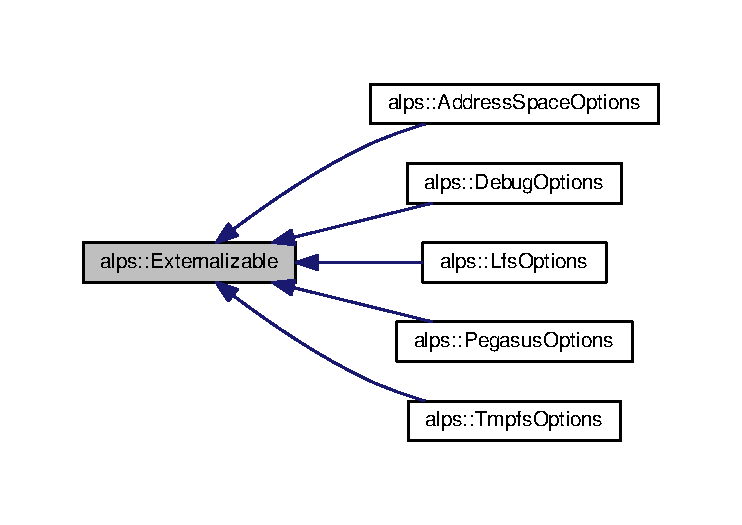
\includegraphics[width=350pt]{structalps_1_1Externalizable__inherit__graph}
\end{center}
\end{figure}
\subsection*{Public Member Functions}
\begin{DoxyCompactItemize}
\item 
virtual \hyperlink{classalps_1_1ErrorStack}{Error\+Stack} \hyperlink{structalps_1_1Externalizable_a3f29cb41a5b5201a1316480087902eed}{load} (Y\+A\+M\+L\+::\+Node $\ast$node, bool ignore\+\_\+missing=false)=0
\begin{DoxyCompactList}\small\item\em Reads the content of this object from the given Y\+A\+ML element. \end{DoxyCompactList}\item 
virtual \hyperlink{classalps_1_1ErrorStack}{Error\+Stack} \hyperlink{structalps_1_1Externalizable_a17a3cdc895ad343d18fd37ff6efd0aef}{save} (Y\+A\+M\+L\+::\+Emitter $\ast$out) const =0
\begin{DoxyCompactList}\small\item\em Writes the content of this object to the given Y\+A\+ML element. \end{DoxyCompactList}\item 
virtual \hyperlink{classalps_1_1ErrorStack}{Error\+Stack} \hyperlink{structalps_1_1Externalizable_a208181477d819b3023ce80c60d54a730}{add\+\_\+command\+\_\+options} (Command\+Option\+List $\ast$cmdopt)=0\hypertarget{structalps_1_1Externalizable_a208181477d819b3023ce80c60d54a730}{}\label{structalps_1_1Externalizable_a208181477d819b3023ce80c60d54a730}

\begin{DoxyCompactList}\small\item\em Adds command options for parsing. \end{DoxyCompactList}\item 
virtual const char $\ast$ \hyperlink{structalps_1_1Externalizable_a865f0f3245014aafdd3133cc9d912cc5}{get\+\_\+tag\+\_\+name} () const =0
\begin{DoxyCompactList}\small\item\em Returns a Y\+A\+ML tag name for this object as a root element. \end{DoxyCompactList}\item 
virtual void \hyperlink{structalps_1_1Externalizable_a5c289543724fdeff9b260f0d0db90f79}{assign} (const \hyperlink{structalps_1_1Externalizable}{alps\+::\+Externalizable} $\ast$other)=0
\begin{DoxyCompactList}\small\item\em Polymorphic assign operator. This should invoke operator= of the derived class. \end{DoxyCompactList}\item 
\hyperlink{classalps_1_1ErrorStack}{Error\+Stack} \hyperlink{structalps_1_1Externalizable_a3841c50c774b365f37d5adffd73d9951}{load\+\_\+from\+\_\+string} (const std\+::string \&yaml, bool ignore\+\_\+missing=false)
\begin{DoxyCompactList}\small\item\em Load the content of this object from the given Y\+A\+ML string. \end{DoxyCompactList}\item 
void \hyperlink{structalps_1_1Externalizable_abba9ffdd2e669137e214e5a499860b04}{save\+\_\+to\+\_\+stream} (std\+::ostream $\ast$ptr) const 
\begin{DoxyCompactList}\small\item\em Invokes \hyperlink{structalps_1_1Externalizable_a17a3cdc895ad343d18fd37ff6efd0aef}{save()} and directs the resulting Y\+A\+ML text to the given stream. \end{DoxyCompactList}\item 
\hyperlink{classalps_1_1ErrorStack}{Error\+Stack} \hyperlink{structalps_1_1Externalizable_a5793ccfb5fd521a3eb8dbde9764c1564}{load\+\_\+from\+\_\+file} (const fs\+::path \&path, bool ignore\+\_\+missing=false)
\begin{DoxyCompactList}\small\item\em Load the content of this object from the specified Y\+A\+ML file. \end{DoxyCompactList}\item 
\hyperlink{classalps_1_1ErrorStack}{Error\+Stack} \hyperlink{structalps_1_1Externalizable_a307766812750ba20517950d0caf554ae}{save\+\_\+to\+\_\+file} (const fs\+::path \&path) const 
\begin{DoxyCompactList}\small\item\em Atomically and durably writes out this object to the specified Y\+A\+ML file. \end{DoxyCompactList}\item 
\hyperlink{classalps_1_1ErrorStack}{Error\+Stack} \hyperlink{structalps_1_1Externalizable_abf8a8a68cc0fc81aa8fec5b7d4092253}{load\+\_\+from\+\_\+command\+\_\+options} (int argc, char $\ast$argv\mbox{[}$\,$\mbox{]})
\begin{DoxyCompactList}\small\item\em Load content from command line options. \end{DoxyCompactList}\end{DoxyCompactItemize}
\subsection*{Static Public Member Functions}
\begin{DoxyCompactItemize}
\item 
static \hyperlink{classalps_1_1ErrorStack}{Error\+Stack} {\bfseries insert\+\_\+comment} (Y\+A\+M\+L\+::\+Emitter $\ast$out, const std\+::string \&comment)\hypertarget{structalps_1_1Externalizable_a28dd65d2a42ab29bd43e558068823724}{}\label{structalps_1_1Externalizable_a28dd65d2a42ab29bd43e558068823724}

\item 
static \hyperlink{classalps_1_1ErrorStack}{Error\+Stack} {\bfseries append\+\_\+comment} (Y\+A\+M\+L\+::\+Emitter $\ast$parent, const std\+::string \&comment)\hypertarget{structalps_1_1Externalizable_acc02665189c05b0bb47cfb47f6cc158f}{}\label{structalps_1_1Externalizable_acc02665189c05b0bb47cfb47f6cc158f}

\item 
{\footnotesize template$<$typename T $>$ }\\static \hyperlink{classalps_1_1ErrorStack}{Error\+Stack} \hyperlink{structalps_1_1Externalizable_a61f858f84debb03b04172d1a4b1f8fd2}{add\+\_\+element} (Y\+A\+M\+L\+::\+Emitter $\ast$out, const std\+::string \&tag, const std\+::string \&comment, T value, bool seq=false)
\item 
{\footnotesize template$<$typename T $>$ }\\static \hyperlink{classalps_1_1ErrorStack}{Error\+Stack} \hyperlink{structalps_1_1Externalizable_a8cffba39c5316b4adbf46e4a9244d2d8}{add\+\_\+element} (Y\+A\+M\+L\+::\+Emitter $\ast$out, const std\+::string \&tag, const std\+::string \&comment, const std\+::vector$<$ T $>$ \&value, bool seq=true)
\item 
{\footnotesize template$<$typename E\+N\+UM $>$ }\\static \hyperlink{classalps_1_1ErrorStack}{Error\+Stack} \hyperlink{structalps_1_1Externalizable_a6a684727a7e58fe41fba41b54ee95e7c}{add\+\_\+enum\+\_\+element} (Y\+A\+M\+L\+::\+Emitter $\ast$out, const std\+::string \&tag, const std\+::string \&comment, E\+N\+UM value)
\item 
static \hyperlink{classalps_1_1ErrorStack}{Error\+Stack} \hyperlink{structalps_1_1Externalizable_acf463dfeffb23bd455eaf868d2e20de6}{add\+\_\+child\+\_\+element} (Y\+A\+M\+L\+::\+Node $\ast$parent, const std\+::string \&tag, const std\+::string \&comment, const \hyperlink{structalps_1_1Externalizable}{Externalizable} \&child)
\item 
{\footnotesize template$<$typename T $>$ }\\static \hyperlink{classalps_1_1ErrorStack}{Error\+Stack} \hyperlink{structalps_1_1Externalizable_a880beff849c59fe09e4be608901ca5e3}{get\+\_\+element} (Y\+A\+M\+L\+::\+Node $\ast$parent, const std\+::string \&tag, T $\ast$out, bool ignore\+\_\+missing=false, bool optional=false, T value=0)
\item 
static \hyperlink{classalps_1_1ErrorStack}{Error\+Stack} \hyperlink{structalps_1_1Externalizable_a53b7384d8b707667d22cf293a4307a73}{get\+\_\+element} (Y\+A\+M\+L\+::\+Node $\ast$parent, const std\+::string \&tag, std\+::string $\ast$out, bool ignore\+\_\+missing=false, bool optional=false, const char $\ast$value=\char`\"{}\char`\"{})
\item 
{\footnotesize template$<$typename E\+N\+UM $>$ }\\static \hyperlink{classalps_1_1ErrorStack}{Error\+Stack} \hyperlink{structalps_1_1Externalizable_a88cbbc7033b72b78fea4dd6fc8ca1402}{get\+\_\+enum\+\_\+element} (Y\+A\+M\+L\+::\+Node $\ast$parent, const std\+::string \&tag, E\+N\+UM $\ast$out, bool ignore\+\_\+missing=false, bool optional=false, E\+N\+UM default\+\_\+value=static\+\_\+cast$<$ E\+N\+UM $>$(0))
\item 
{\footnotesize template$<$typename S\+I\+ZE $>$ }\\static \hyperlink{classalps_1_1ErrorStack}{Error\+Stack} \hyperlink{structalps_1_1Externalizable_a1a6df09ad89c2154cc94de784127ec1f}{get\+\_\+size\+\_\+element} (Y\+A\+M\+L\+::\+Node $\ast$parent, const std\+::string \&tag, S\+I\+ZE $\ast$out, bool ignore\+\_\+missing=false, bool optional=false, S\+I\+ZE default\+\_\+value=static\+\_\+cast$<$ S\+I\+ZE $>$(0))
\item 
{\footnotesize template$<$typename T $>$ }\\static \hyperlink{classalps_1_1ErrorStack}{Error\+Stack} \hyperlink{structalps_1_1Externalizable_a02ca000360b9ab5fc30b4cf30ade1354}{get\+\_\+element} (Y\+A\+M\+L\+::\+Node $\ast$parent, const std\+::string \&tag, std\+::vector$<$ T $>$ $\ast$out, bool ignore\+\_\+missing=false, bool optional=false)
\item 
static \hyperlink{classalps_1_1ErrorStack}{Error\+Stack} \hyperlink{structalps_1_1Externalizable_a03e9ab31323b870ba49408a9cd2720bc}{get\+\_\+child\+\_\+element} (Y\+A\+M\+L\+::\+Node $\ast$parent, const std\+::string \&tag, \hyperlink{structalps_1_1Externalizable}{Externalizable} $\ast$child, bool ignore\+\_\+missing=false, bool optional=false)
\item 
{\footnotesize template$<$typename T $>$ }\\static \hyperlink{classalps_1_1ErrorStack}{Error\+Stack} {\bfseries add\+\_\+command\+\_\+option} (Command\+Option\+List $\ast$cmdlist, const std\+::string \&tag, T $\ast$out, std\+::string desc)\hypertarget{structalps_1_1Externalizable_a6a54f3965c85284e18b2d2acdb936f59}{}\label{structalps_1_1Externalizable_a6a54f3965c85284e18b2d2acdb936f59}

\end{DoxyCompactItemize}


\subsection{Detailed Description}
Derived classes must implement \hyperlink{structalps_1_1Externalizable_a3f29cb41a5b5201a1316480087902eed}{load()} and \hyperlink{structalps_1_1Externalizable_a17a3cdc895ad343d18fd37ff6efd0aef}{save()}. 

\subsection{Member Function Documentation}
\index{alps\+::\+Externalizable@{alps\+::\+Externalizable}!add\+\_\+child\+\_\+element@{add\+\_\+child\+\_\+element}}
\index{add\+\_\+child\+\_\+element@{add\+\_\+child\+\_\+element}!alps\+::\+Externalizable@{alps\+::\+Externalizable}}
\subsubsection[{\texorpdfstring{add\+\_\+child\+\_\+element(\+Y\+A\+M\+L\+::\+Node $\ast$parent, const std\+::string \&tag, const std\+::string \&comment, const Externalizable \&child)}{add_child_element(YAML::Node *parent, const std::string &tag, const std::string &comment, const Externalizable &child)}}]{\setlength{\rightskip}{0pt plus 5cm}static {\bf Error\+Stack} alps\+::\+Externalizable\+::add\+\_\+child\+\_\+element (
\begin{DoxyParamCaption}
\item[{Y\+A\+M\+L\+::\+Node $\ast$}]{parent, }
\item[{const std\+::string \&}]{tag, }
\item[{const std\+::string \&}]{comment, }
\item[{const {\bf Externalizable} \&}]{child}
\end{DoxyParamCaption}
)\hspace{0.3cm}{\ttfamily [static]}}\hypertarget{structalps_1_1Externalizable_acf463dfeffb23bd455eaf868d2e20de6}{}\label{structalps_1_1Externalizable_acf463dfeffb23bd455eaf868d2e20de6}
child \hyperlink{structalps_1_1Externalizable}{Externalizable} version \index{alps\+::\+Externalizable@{alps\+::\+Externalizable}!add\+\_\+element@{add\+\_\+element}}
\index{add\+\_\+element@{add\+\_\+element}!alps\+::\+Externalizable@{alps\+::\+Externalizable}}
\subsubsection[{\texorpdfstring{add\+\_\+element(\+Y\+A\+M\+L\+::\+Emitter $\ast$out, const std\+::string \&tag, const std\+::string \&comment, T value, bool seq=false)}{add_element(YAML::Emitter *out, const std::string &tag, const std::string &comment, T value, bool seq=false)}}]{\setlength{\rightskip}{0pt plus 5cm}template$<$typename T $>$ {\bf Error\+Stack} alps\+::\+Externalizable\+::add\+\_\+element (
\begin{DoxyParamCaption}
\item[{Y\+A\+M\+L\+::\+Emitter $\ast$}]{out, }
\item[{const std\+::string \&}]{tag, }
\item[{const std\+::string \&}]{comment, }
\item[{T}]{value, }
\item[{bool}]{seq = {\ttfamily false}}
\end{DoxyParamCaption}
)\hspace{0.3cm}{\ttfamily [static]}}\hypertarget{structalps_1_1Externalizable_a61f858f84debb03b04172d1a4b1f8fd2}{}\label{structalps_1_1Externalizable_a61f858f84debb03b04172d1a4b1f8fd2}
Only declaration in header. Explicitly instantiated in cpp for each type this func handles. \index{alps\+::\+Externalizable@{alps\+::\+Externalizable}!add\+\_\+element@{add\+\_\+element}}
\index{add\+\_\+element@{add\+\_\+element}!alps\+::\+Externalizable@{alps\+::\+Externalizable}}
\subsubsection[{\texorpdfstring{add\+\_\+element(\+Y\+A\+M\+L\+::\+Emitter $\ast$out, const std\+::string \&tag, const std\+::string \&comment, const std\+::vector$<$ T $>$ \&value, bool seq=true)}{add_element(YAML::Emitter *out, const std::string &tag, const std::string &comment, const std::vector< T > &value, bool seq=true)}}]{\setlength{\rightskip}{0pt plus 5cm}template$<$typename T $>$ {\bf Error\+Stack} alps\+::\+Externalizable\+::add\+\_\+element (
\begin{DoxyParamCaption}
\item[{Y\+A\+M\+L\+::\+Emitter $\ast$}]{out, }
\item[{const std\+::string \&}]{tag, }
\item[{const std\+::string \&}]{comment, }
\item[{const std\+::vector$<$ T $>$ \&}]{value, }
\item[{bool}]{seq = {\ttfamily true}}
\end{DoxyParamCaption}
)\hspace{0.3cm}{\ttfamily [static]}}\hypertarget{structalps_1_1Externalizable_a8cffba39c5316b4adbf46e4a9244d2d8}{}\label{structalps_1_1Externalizable_a8cffba39c5316b4adbf46e4a9244d2d8}
vector version

Only declaration in header. Explicitly instantiated in cpp for each type this func handles. \index{alps\+::\+Externalizable@{alps\+::\+Externalizable}!add\+\_\+enum\+\_\+element@{add\+\_\+enum\+\_\+element}}
\index{add\+\_\+enum\+\_\+element@{add\+\_\+enum\+\_\+element}!alps\+::\+Externalizable@{alps\+::\+Externalizable}}
\subsubsection[{\texorpdfstring{add\+\_\+enum\+\_\+element(\+Y\+A\+M\+L\+::\+Emitter $\ast$out, const std\+::string \&tag, const std\+::string \&comment, E\+N\+U\+M value)}{add_enum_element(YAML::Emitter *out, const std::string &tag, const std::string &comment, ENUM value)}}]{\setlength{\rightskip}{0pt plus 5cm}template$<$typename E\+N\+UM $>$ static {\bf Error\+Stack} alps\+::\+Externalizable\+::add\+\_\+enum\+\_\+element (
\begin{DoxyParamCaption}
\item[{Y\+A\+M\+L\+::\+Emitter $\ast$}]{out, }
\item[{const std\+::string \&}]{tag, }
\item[{const std\+::string \&}]{comment, }
\item[{E\+N\+UM}]{value}
\end{DoxyParamCaption}
)\hspace{0.3cm}{\ttfamily [inline]}, {\ttfamily [static]}}\hypertarget{structalps_1_1Externalizable_a6a684727a7e58fe41fba41b54ee95e7c}{}\label{structalps_1_1Externalizable_a6a684727a7e58fe41fba41b54ee95e7c}
enum version \index{alps\+::\+Externalizable@{alps\+::\+Externalizable}!assign@{assign}}
\index{assign@{assign}!alps\+::\+Externalizable@{alps\+::\+Externalizable}}
\subsubsection[{\texorpdfstring{assign(const alps\+::\+Externalizable $\ast$other)=0}{assign(const alps::Externalizable *other)=0}}]{\setlength{\rightskip}{0pt plus 5cm}virtual void alps\+::\+Externalizable\+::assign (
\begin{DoxyParamCaption}
\item[{const {\bf alps\+::\+Externalizable} $\ast$}]{other}
\end{DoxyParamCaption}
)\hspace{0.3cm}{\ttfamily [pure virtual]}}\hypertarget{structalps_1_1Externalizable_a5c289543724fdeff9b260f0d0db90f79}{}\label{structalps_1_1Externalizable_a5c289543724fdeff9b260f0d0db90f79}

\begin{DoxyParams}[1]{Parameters}
\mbox{\tt in}  & {\em other} & assigned value. It must be dynamic-\/castable to the assignee class. \\
\hline
\end{DoxyParams}
\index{alps\+::\+Externalizable@{alps\+::\+Externalizable}!get\+\_\+child\+\_\+element@{get\+\_\+child\+\_\+element}}
\index{get\+\_\+child\+\_\+element@{get\+\_\+child\+\_\+element}!alps\+::\+Externalizable@{alps\+::\+Externalizable}}
\subsubsection[{\texorpdfstring{get\+\_\+child\+\_\+element(\+Y\+A\+M\+L\+::\+Node $\ast$parent, const std\+::string \&tag, Externalizable $\ast$child, bool ignore\+\_\+missing=false, bool optional=false)}{get_child_element(YAML::Node *parent, const std::string &tag, Externalizable *child, bool ignore_missing=false, bool optional=false)}}]{\setlength{\rightskip}{0pt plus 5cm}{\bf Error\+Stack} alps\+::\+Externalizable\+::get\+\_\+child\+\_\+element (
\begin{DoxyParamCaption}
\item[{Y\+A\+M\+L\+::\+Node $\ast$}]{parent, }
\item[{const std\+::string \&}]{tag, }
\item[{{\bf Externalizable} $\ast$}]{child, }
\item[{bool}]{ignore\+\_\+missing = {\ttfamily false}, }
\item[{bool}]{optional = {\ttfamily false}}
\end{DoxyParamCaption}
)\hspace{0.3cm}{\ttfamily [static]}}\hypertarget{structalps_1_1Externalizable_a03e9ab31323b870ba49408a9cd2720bc}{}\label{structalps_1_1Externalizable_a03e9ab31323b870ba49408a9cd2720bc}
child \hyperlink{structalps_1_1Externalizable}{Externalizable} version \index{alps\+::\+Externalizable@{alps\+::\+Externalizable}!get\+\_\+element@{get\+\_\+element}}
\index{get\+\_\+element@{get\+\_\+element}!alps\+::\+Externalizable@{alps\+::\+Externalizable}}
\subsubsection[{\texorpdfstring{get\+\_\+element(\+Y\+A\+M\+L\+::\+Node $\ast$parent, const std\+::string \&tag, T $\ast$out, bool ignore\+\_\+missing=false, bool optional=false, T value=0)}{get_element(YAML::Node *parent, const std::string &tag, T *out, bool ignore_missing=false, bool optional=false, T value=0)}}]{\setlength{\rightskip}{0pt plus 5cm}template$<$typename T $>$ {\bf Error\+Stack} alps\+::\+Externalizable\+::get\+\_\+element (
\begin{DoxyParamCaption}
\item[{Y\+A\+M\+L\+::\+Node $\ast$}]{parent, }
\item[{const std\+::string \&}]{tag, }
\item[{T $\ast$}]{out, }
\item[{bool}]{ignore\+\_\+missing = {\ttfamily false}, }
\item[{bool}]{optional = {\ttfamily false}, }
\item[{T}]{value = {\ttfamily 0}}
\end{DoxyParamCaption}
)\hspace{0.3cm}{\ttfamily [static]}}\hypertarget{structalps_1_1Externalizable_a880beff849c59fe09e4be608901ca5e3}{}\label{structalps_1_1Externalizable_a880beff849c59fe09e4be608901ca5e3}
Only declaration in header. Explicitly instantiated in cpp for each type this func handles. \index{alps\+::\+Externalizable@{alps\+::\+Externalizable}!get\+\_\+element@{get\+\_\+element}}
\index{get\+\_\+element@{get\+\_\+element}!alps\+::\+Externalizable@{alps\+::\+Externalizable}}
\subsubsection[{\texorpdfstring{get\+\_\+element(\+Y\+A\+M\+L\+::\+Node $\ast$parent, const std\+::string \&tag, std\+::string $\ast$out, bool ignore\+\_\+missing=false, bool optional=false, const char $\ast$value="""")}{get_element(YAML::Node *parent, const std::string &tag, std::string *out, bool ignore_missing=false, bool optional=false, const char *value="")}}]{\setlength{\rightskip}{0pt plus 5cm}{\bf Error\+Stack} alps\+::\+Externalizable\+::get\+\_\+element (
\begin{DoxyParamCaption}
\item[{Y\+A\+M\+L\+::\+Node $\ast$}]{parent, }
\item[{const std\+::string \&}]{tag, }
\item[{std\+::string $\ast$}]{out, }
\item[{bool}]{ignore\+\_\+missing = {\ttfamily false}, }
\item[{bool}]{optional = {\ttfamily false}, }
\item[{const char $\ast$}]{value = {\ttfamily \char`\"{}\char`\"{}}}
\end{DoxyParamCaption}
)\hspace{0.3cm}{\ttfamily [static]}}\hypertarget{structalps_1_1Externalizable_a53b7384d8b707667d22cf293a4307a73}{}\label{structalps_1_1Externalizable_a53b7384d8b707667d22cf293a4307a73}
string type is bit special. \index{alps\+::\+Externalizable@{alps\+::\+Externalizable}!get\+\_\+element@{get\+\_\+element}}
\index{get\+\_\+element@{get\+\_\+element}!alps\+::\+Externalizable@{alps\+::\+Externalizable}}
\subsubsection[{\texorpdfstring{get\+\_\+element(\+Y\+A\+M\+L\+::\+Node $\ast$parent, const std\+::string \&tag, std\+::vector$<$ T $>$ $\ast$out, bool ignore\+\_\+missing=false, bool optional=false)}{get_element(YAML::Node *parent, const std::string &tag, std::vector< T > *out, bool ignore_missing=false, bool optional=false)}}]{\setlength{\rightskip}{0pt plus 5cm}template$<$typename T $>$ {\bf Error\+Stack} alps\+::\+Externalizable\+::get\+\_\+element (
\begin{DoxyParamCaption}
\item[{Y\+A\+M\+L\+::\+Node $\ast$}]{parent, }
\item[{const std\+::string \&}]{tag, }
\item[{std\+::vector$<$ T $>$ $\ast$}]{out, }
\item[{bool}]{ignore\+\_\+missing = {\ttfamily false}, }
\item[{bool}]{optional = {\ttfamily false}}
\end{DoxyParamCaption}
)\hspace{0.3cm}{\ttfamily [static]}}\hypertarget{structalps_1_1Externalizable_a02ca000360b9ab5fc30b4cf30ade1354}{}\label{structalps_1_1Externalizable_a02ca000360b9ab5fc30b4cf30ade1354}
vector version. Only declaration in header. Explicitly instantiated in cpp for each type this func handles. \index{alps\+::\+Externalizable@{alps\+::\+Externalizable}!get\+\_\+enum\+\_\+element@{get\+\_\+enum\+\_\+element}}
\index{get\+\_\+enum\+\_\+element@{get\+\_\+enum\+\_\+element}!alps\+::\+Externalizable@{alps\+::\+Externalizable}}
\subsubsection[{\texorpdfstring{get\+\_\+enum\+\_\+element(\+Y\+A\+M\+L\+::\+Node $\ast$parent, const std\+::string \&tag, E\+N\+U\+M $\ast$out, bool ignore\+\_\+missing=false, bool optional=false, E\+N\+U\+M default\+\_\+value=static\+\_\+cast$<$ E\+N\+U\+M $>$(0))}{get_enum_element(YAML::Node *parent, const std::string &tag, ENUM *out, bool ignore_missing=false, bool optional=false, ENUM default_value=static_cast< ENUM >(0))}}]{\setlength{\rightskip}{0pt plus 5cm}template$<$typename E\+N\+UM $>$ static {\bf Error\+Stack} alps\+::\+Externalizable\+::get\+\_\+enum\+\_\+element (
\begin{DoxyParamCaption}
\item[{Y\+A\+M\+L\+::\+Node $\ast$}]{parent, }
\item[{const std\+::string \&}]{tag, }
\item[{E\+N\+UM $\ast$}]{out, }
\item[{bool}]{ignore\+\_\+missing = {\ttfamily false}, }
\item[{bool}]{optional = {\ttfamily false}, }
\item[{E\+N\+UM}]{default\+\_\+value = {\ttfamily static\+\_\+cast$<$ENUM$>$(0)}}
\end{DoxyParamCaption}
)\hspace{0.3cm}{\ttfamily [inline]}, {\ttfamily [static]}}\hypertarget{structalps_1_1Externalizable_a88cbbc7033b72b78fea4dd6fc8ca1402}{}\label{structalps_1_1Externalizable_a88cbbc7033b72b78fea4dd6fc8ca1402}
enum version \index{alps\+::\+Externalizable@{alps\+::\+Externalizable}!get\+\_\+size\+\_\+element@{get\+\_\+size\+\_\+element}}
\index{get\+\_\+size\+\_\+element@{get\+\_\+size\+\_\+element}!alps\+::\+Externalizable@{alps\+::\+Externalizable}}
\subsubsection[{\texorpdfstring{get\+\_\+size\+\_\+element(\+Y\+A\+M\+L\+::\+Node $\ast$parent, const std\+::string \&tag, S\+I\+Z\+E $\ast$out, bool ignore\+\_\+missing=false, bool optional=false, S\+I\+Z\+E default\+\_\+value=static\+\_\+cast$<$ S\+I\+Z\+E $>$(0))}{get_size_element(YAML::Node *parent, const std::string &tag, SIZE *out, bool ignore_missing=false, bool optional=false, SIZE default_value=static_cast< SIZE >(0))}}]{\setlength{\rightskip}{0pt plus 5cm}template$<$typename S\+I\+ZE $>$ static {\bf Error\+Stack} alps\+::\+Externalizable\+::get\+\_\+size\+\_\+element (
\begin{DoxyParamCaption}
\item[{Y\+A\+M\+L\+::\+Node $\ast$}]{parent, }
\item[{const std\+::string \&}]{tag, }
\item[{S\+I\+ZE $\ast$}]{out, }
\item[{bool}]{ignore\+\_\+missing = {\ttfamily false}, }
\item[{bool}]{optional = {\ttfamily false}, }
\item[{S\+I\+ZE}]{default\+\_\+value = {\ttfamily static\+\_\+cast$<$SIZE$>$(0)}}
\end{DoxyParamCaption}
)\hspace{0.3cm}{\ttfamily [inline]}, {\ttfamily [static]}}\hypertarget{structalps_1_1Externalizable_a1a6df09ad89c2154cc94de784127ec1f}{}\label{structalps_1_1Externalizable_a1a6df09ad89c2154cc94de784127ec1f}
size version \index{alps\+::\+Externalizable@{alps\+::\+Externalizable}!get\+\_\+tag\+\_\+name@{get\+\_\+tag\+\_\+name}}
\index{get\+\_\+tag\+\_\+name@{get\+\_\+tag\+\_\+name}!alps\+::\+Externalizable@{alps\+::\+Externalizable}}
\subsubsection[{\texorpdfstring{get\+\_\+tag\+\_\+name() const =0}{get_tag_name() const =0}}]{\setlength{\rightskip}{0pt plus 5cm}virtual const char$\ast$ alps\+::\+Externalizable\+::get\+\_\+tag\+\_\+name (
\begin{DoxyParamCaption}
{}
\end{DoxyParamCaption}
) const\hspace{0.3cm}{\ttfamily [pure virtual]}}\hypertarget{structalps_1_1Externalizable_a865f0f3245014aafdd3133cc9d912cc5}{}\label{structalps_1_1Externalizable_a865f0f3245014aafdd3133cc9d912cc5}
We might want to give a different name for same externalizable objects, so this is used only when it is the root element of yaml. \index{alps\+::\+Externalizable@{alps\+::\+Externalizable}!load@{load}}
\index{load@{load}!alps\+::\+Externalizable@{alps\+::\+Externalizable}}
\subsubsection[{\texorpdfstring{load(\+Y\+A\+M\+L\+::\+Node $\ast$node, bool ignore\+\_\+missing=false)=0}{load(YAML::Node *node, bool ignore_missing=false)=0}}]{\setlength{\rightskip}{0pt plus 5cm}virtual {\bf Error\+Stack} alps\+::\+Externalizable\+::load (
\begin{DoxyParamCaption}
\item[{Y\+A\+M\+L\+::\+Node $\ast$}]{node, }
\item[{bool}]{ignore\+\_\+missing = {\ttfamily false}}
\end{DoxyParamCaption}
)\hspace{0.3cm}{\ttfamily [pure virtual]}}\hypertarget{structalps_1_1Externalizable_a3f29cb41a5b5201a1316480087902eed}{}\label{structalps_1_1Externalizable_a3f29cb41a5b5201a1316480087902eed}

\begin{DoxyParams}[1]{Parameters}
\mbox{\tt in}  & {\em node} & the Y\+A\+ML node that represents this object\\
\hline
\end{DoxyParams}
Expect errors due to missing-\/elements, out-\/of-\/range values, etc. \index{alps\+::\+Externalizable@{alps\+::\+Externalizable}!load\+\_\+from\+\_\+command\+\_\+options@{load\+\_\+from\+\_\+command\+\_\+options}}
\index{load\+\_\+from\+\_\+command\+\_\+options@{load\+\_\+from\+\_\+command\+\_\+options}!alps\+::\+Externalizable@{alps\+::\+Externalizable}}
\subsubsection[{\texorpdfstring{load\+\_\+from\+\_\+command\+\_\+options(int argc, char $\ast$argv[])}{load_from_command_options(int argc, char *argv[])}}]{\setlength{\rightskip}{0pt plus 5cm}{\bf Error\+Stack} alps\+::\+Externalizable\+::load\+\_\+from\+\_\+command\+\_\+options (
\begin{DoxyParamCaption}
\item[{int}]{argc, }
\item[{char $\ast$}]{argv\mbox{[}$\,$\mbox{]}}
\end{DoxyParamCaption}
)}\hypertarget{structalps_1_1Externalizable_abf8a8a68cc0fc81aa8fec5b7d4092253}{}\label{structalps_1_1Externalizable_abf8a8a68cc0fc81aa8fec5b7d4092253}

\begin{DoxyParams}[1]{Parameters}
\mbox{\tt in}  & {\em argc} & number of strings that make up the command line. \\
\hline
\mbox{\tt in}  & {\em argv} & arguments passed to a program through the command line.\\
\hline
\end{DoxyParams}
Expect errors due to missing-\/elements, out-\/of-\/range values, etc. \index{alps\+::\+Externalizable@{alps\+::\+Externalizable}!load\+\_\+from\+\_\+file@{load\+\_\+from\+\_\+file}}
\index{load\+\_\+from\+\_\+file@{load\+\_\+from\+\_\+file}!alps\+::\+Externalizable@{alps\+::\+Externalizable}}
\subsubsection[{\texorpdfstring{load\+\_\+from\+\_\+file(const fs\+::path \&path, bool ignore\+\_\+missing=false)}{load_from_file(const fs::path &path, bool ignore_missing=false)}}]{\setlength{\rightskip}{0pt plus 5cm}{\bf Error\+Stack} alps\+::\+Externalizable\+::load\+\_\+from\+\_\+file (
\begin{DoxyParamCaption}
\item[{const fs\+::path \&}]{path, }
\item[{bool}]{ignore\+\_\+missing = {\ttfamily false}}
\end{DoxyParamCaption}
)}\hypertarget{structalps_1_1Externalizable_a5793ccfb5fd521a3eb8dbde9764c1564}{}\label{structalps_1_1Externalizable_a5793ccfb5fd521a3eb8dbde9764c1564}

\begin{DoxyParams}[1]{Parameters}
\mbox{\tt in}  & {\em path} & path of the Y\+A\+ML file. \\
\hline
\mbox{\tt in}  & {\em ignore\+\_\+missing} & whether to ignore missing options.\\
\hline
\end{DoxyParams}
Expect errors due to missing-\/elements, out-\/of-\/range values, etc. \index{alps\+::\+Externalizable@{alps\+::\+Externalizable}!load\+\_\+from\+\_\+string@{load\+\_\+from\+\_\+string}}
\index{load\+\_\+from\+\_\+string@{load\+\_\+from\+\_\+string}!alps\+::\+Externalizable@{alps\+::\+Externalizable}}
\subsubsection[{\texorpdfstring{load\+\_\+from\+\_\+string(const std\+::string \&yaml, bool ignore\+\_\+missing=false)}{load_from_string(const std::string &yaml, bool ignore_missing=false)}}]{\setlength{\rightskip}{0pt plus 5cm}{\bf Error\+Stack} alps\+::\+Externalizable\+::load\+\_\+from\+\_\+string (
\begin{DoxyParamCaption}
\item[{const std\+::string \&}]{yaml, }
\item[{bool}]{ignore\+\_\+missing = {\ttfamily false}}
\end{DoxyParamCaption}
)}\hypertarget{structalps_1_1Externalizable_a3841c50c774b365f37d5adffd73d9951}{}\label{structalps_1_1Externalizable_a3841c50c774b365f37d5adffd73d9951}

\begin{DoxyParams}[1]{Parameters}
\mbox{\tt in}  & {\em yaml} & Y\+A\+ML string. \\
\hline
\mbox{\tt in}  & {\em ignore\+\_\+missing} & whether to ignore missing options.\\
\hline
\end{DoxyParams}
Expect errors due to missing-\/elements, out-\/of-\/range values, etc. \index{alps\+::\+Externalizable@{alps\+::\+Externalizable}!save@{save}}
\index{save@{save}!alps\+::\+Externalizable@{alps\+::\+Externalizable}}
\subsubsection[{\texorpdfstring{save(\+Y\+A\+M\+L\+::\+Emitter $\ast$out) const =0}{save(YAML::Emitter *out) const =0}}]{\setlength{\rightskip}{0pt plus 5cm}virtual {\bf Error\+Stack} alps\+::\+Externalizable\+::save (
\begin{DoxyParamCaption}
\item[{Y\+A\+M\+L\+::\+Emitter $\ast$}]{out}
\end{DoxyParamCaption}
) const\hspace{0.3cm}{\ttfamily [pure virtual]}}\hypertarget{structalps_1_1Externalizable_a17a3cdc895ad343d18fd37ff6efd0aef}{}\label{structalps_1_1Externalizable_a17a3cdc895ad343d18fd37ff6efd0aef}

\begin{DoxyParams}[1]{Parameters}
\mbox{\tt in}  & {\em node} & the Y\+A\+ML node that represents this object\\
\hline
\end{DoxyParams}
Expect only out-\/of-\/memory error. We receive the Y\+A\+ML node this object will represent, so this method does not determine the Y\+A\+ML node name of itself. The parent object determines children\textquotesingle{}s tag names because one parent object might have multiple child objects of the same type with different Y\+A\+ML element name. \index{alps\+::\+Externalizable@{alps\+::\+Externalizable}!save\+\_\+to\+\_\+file@{save\+\_\+to\+\_\+file}}
\index{save\+\_\+to\+\_\+file@{save\+\_\+to\+\_\+file}!alps\+::\+Externalizable@{alps\+::\+Externalizable}}
\subsubsection[{\texorpdfstring{save\+\_\+to\+\_\+file(const fs\+::path \&path) const }{save_to_file(const fs::path &path) const }}]{\setlength{\rightskip}{0pt plus 5cm}{\bf Error\+Stack} alps\+::\+Externalizable\+::save\+\_\+to\+\_\+file (
\begin{DoxyParamCaption}
\item[{const fs\+::path \&}]{path}
\end{DoxyParamCaption}
) const}\hypertarget{structalps_1_1Externalizable_a307766812750ba20517950d0caf554ae}{}\label{structalps_1_1Externalizable_a307766812750ba20517950d0caf554ae}

\begin{DoxyParams}[1]{Parameters}
\mbox{\tt in}  & {\em path} & path of the Y\+A\+ML file.\\
\hline
\end{DoxyParams}
If the file exists, this method atomically overwrites it via P\+O\+S\+IX\textquotesingle{}s atomic rename semantics. If the parent folder doesn\textquotesingle{}t exist, this method automatically creates the folder. Expect errors due to file-\/permission (and other file I/O issue), out-\/of-\/memory, etc. \index{alps\+::\+Externalizable@{alps\+::\+Externalizable}!save\+\_\+to\+\_\+stream@{save\+\_\+to\+\_\+stream}}
\index{save\+\_\+to\+\_\+stream@{save\+\_\+to\+\_\+stream}!alps\+::\+Externalizable@{alps\+::\+Externalizable}}
\subsubsection[{\texorpdfstring{save\+\_\+to\+\_\+stream(std\+::ostream $\ast$ptr) const }{save_to_stream(std::ostream *ptr) const }}]{\setlength{\rightskip}{0pt plus 5cm}void alps\+::\+Externalizable\+::save\+\_\+to\+\_\+stream (
\begin{DoxyParamCaption}
\item[{std\+::ostream $\ast$}]{ptr}
\end{DoxyParamCaption}
) const}\hypertarget{structalps_1_1Externalizable_abba9ffdd2e669137e214e5a499860b04}{}\label{structalps_1_1Externalizable_abba9ffdd2e669137e214e5a499860b04}

\begin{DoxyParams}[1]{Parameters}
\mbox{\tt in}  & {\em ptr} & ostream to write to. \\
\hline
\end{DoxyParams}


The documentation for this struct was generated from the following files\+:\begin{DoxyCompactItemize}
\item 
/home/yuan/\+Benchmarks/whisper/mnemosyne-\/gcc/usermode/library/pmalloc/include/alps/include/alps/common/externalizable.\+hh\item 
/home/yuan/\+Benchmarks/whisper/mnemosyne-\/gcc/usermode/library/pmalloc/include/alps/src/common/externalizable.\+cc\end{DoxyCompactItemize}

\hypertarget{classalps_1_1FileSystemTypeFactory}{}\section{alps\+:\+:File\+System\+Type\+Factory$<$ Object\+Type $>$ Class Template Reference}
\label{classalps_1_1FileSystemTypeFactory}\index{alps\+::\+File\+System\+Type\+Factory$<$ Object\+Type $>$@{alps\+::\+File\+System\+Type\+Factory$<$ Object\+Type $>$}}


A factory class for constructing objects based on the type of the underlying file system.  




{\ttfamily \#include $<$fstype\+\_\+factory.\+hh$>$}



Collaboration diagram for alps\+:\+:File\+System\+Type\+Factory$<$ Object\+Type $>$\+:
\nopagebreak
\begin{figure}[H]
\begin{center}
\leavevmode
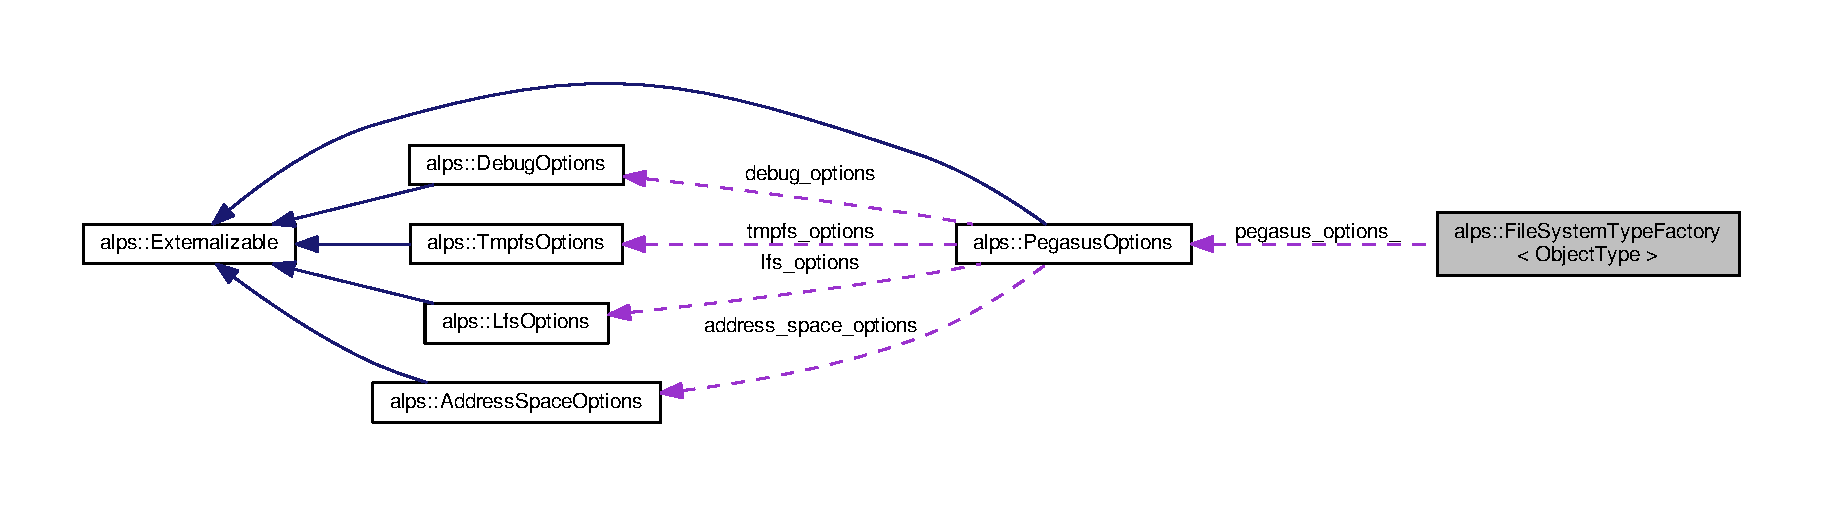
\includegraphics[width=350pt]{classalps_1_1FileSystemTypeFactory__coll__graph}
\end{center}
\end{figure}
\subsection*{Public Types}
\begin{DoxyCompactItemize}
\item 
typedef Object\+Type $\ast$($\ast$ {\bfseries Construct\+Callback}) (const boost\+::filesystem\+::path \&pathname, const \hyperlink{structalps_1_1PegasusOptions}{Pegasus\+Options} \&pegasus\+\_\+options)\hypertarget{classalps_1_1FileSystemTypeFactory_ac969de7bdc5ea5846adb111c9b00154c}{}\label{classalps_1_1FileSystemTypeFactory_ac969de7bdc5ea5846adb111c9b00154c}

\end{DoxyCompactItemize}
\subsection*{Public Member Functions}
\begin{DoxyCompactItemize}
\item 
{\bfseries File\+System\+Type\+Factory} (const \hyperlink{structalps_1_1PegasusOptions}{Pegasus\+Options} \&pegasus\+\_\+options)\hypertarget{classalps_1_1FileSystemTypeFactory_a1466c1689d4b9c4da885524fab0c4c61}{}\label{classalps_1_1FileSystemTypeFactory_a1466c1689d4b9c4da885524fab0c4c61}

\item 
\hyperlink{group__ERRORCODES_ga6263a3c9a0b8d36aea21cdd835ac99fe}{Error\+Code} {\bfseries construct} (const boost\+::filesystem\+::path \&pathname, Object\+Type $\ast$$\ast$object)\hypertarget{classalps_1_1FileSystemTypeFactory_ad29eb6817e32392477d54bb8d4a00a5b}{}\label{classalps_1_1FileSystemTypeFactory_ad29eb6817e32392477d54bb8d4a00a5b}

\item 
\hyperlink{group__ERRORCODES_ga6263a3c9a0b8d36aea21cdd835ac99fe}{Error\+Code} {\bfseries register\+\_\+fstype} (const std\+::string \&fstype, Construct\+Callback)\hypertarget{classalps_1_1FileSystemTypeFactory_aeb8d8c62187c4d6a9338be6b7bd2cec4}{}\label{classalps_1_1FileSystemTypeFactory_aeb8d8c62187c4d6a9338be6b7bd2cec4}

\end{DoxyCompactItemize}
\subsection*{Protected Attributes}
\begin{DoxyCompactItemize}
\item 
Construct\+Callback\+Map {\bfseries callbacks\+\_\+}\hypertarget{classalps_1_1FileSystemTypeFactory_ab0e19021185da56a6b7c4c3c9c30a346}{}\label{classalps_1_1FileSystemTypeFactory_ab0e19021185da56a6b7c4c3c9c30a346}

\item 
\hyperlink{structalps_1_1PegasusOptions}{Pegasus\+Options} {\bfseries pegasus\+\_\+options\+\_\+}\hypertarget{classalps_1_1FileSystemTypeFactory_a7a2c7e28160c6a42fa56c2f695766be5}{}\label{classalps_1_1FileSystemTypeFactory_a7a2c7e28160c6a42fa56c2f695766be5}

\end{DoxyCompactItemize}


The documentation for this class was generated from the following file\+:\begin{DoxyCompactItemize}
\item 
/home/yuan/\+Benchmarks/whisper/mnemosyne-\/gcc/usermode/library/pmalloc/include/alps/src/pegasus/fstype\+\_\+factory.\+hh\end{DoxyCompactItemize}

\hypertarget{classalps_1_1FRDNode}{}\section{alps\+:\+:F\+R\+D\+Node Class Reference}
\label{classalps_1_1FRDNode}\index{alps\+::\+F\+R\+D\+Node@{alps\+::\+F\+R\+D\+Node}}
\subsection*{Public Member Functions}
\begin{DoxyCompactItemize}
\item 
{\bfseries F\+R\+D\+Node} (unsigned int node\+\_\+id)\hypertarget{classalps_1_1FRDNode_a3bab23a8d25a3aecf06bafced43f5394}{}\label{classalps_1_1FRDNode_a3bab23a8d25a3aecf06bafced43f5394}

\item 
{\bfseries F\+R\+D\+Node} (unsigned int rack, unsigned int encl, unsigned int node)\hypertarget{classalps_1_1FRDNode_a29d2b46be6d598d1262662ee00a1495f}{}\label{classalps_1_1FRDNode_a29d2b46be6d598d1262662ee00a1495f}

\item 
unsigned int {\bfseries id} () const \hypertarget{classalps_1_1FRDNode_a0f843bde69e69062910ac352a68961e1}{}\label{classalps_1_1FRDNode_a0f843bde69e69062910ac352a68961e1}

\item 
bool {\bfseries operator==} (const \hyperlink{classalps_1_1FRDNode}{F\+R\+D\+Node} \&other)\hypertarget{classalps_1_1FRDNode_a845638568988450a40434397d8711e2d}{}\label{classalps_1_1FRDNode_a845638568988450a40434397d8711e2d}

\item 
bool {\bfseries operator!=} (const \hyperlink{classalps_1_1FRDNode}{F\+R\+D\+Node} \&other)\hypertarget{classalps_1_1FRDNode_a1a9b1c9cef0d692a8977f3f5bb9979c5}{}\label{classalps_1_1FRDNode_a1a9b1c9cef0d692a8977f3f5bb9979c5}

\item 
unsigned int {\bfseries operator-\/} (const \hyperlink{classalps_1_1FRDNode}{F\+R\+D\+Node} \&other)\hypertarget{classalps_1_1FRDNode_a2bae6e2d65b67c6ded12dcf5ae6e1226}{}\label{classalps_1_1FRDNode_a2bae6e2d65b67c6ded12dcf5ae6e1226}

\end{DoxyCompactItemize}


The documentation for this class was generated from the following file\+:\begin{DoxyCompactItemize}
\item 
/home/yuan/\+Benchmarks/whisper/mnemosyne-\/gcc/usermode/library/pmalloc/include/alps/src/pegasus/lfs\+\_\+topology.\+hh\end{DoxyCompactItemize}

\hypertarget{structalps_1_1BacktraceContext_1_1GlibcBacktraceInfo}{}\section{alps\+:\+:Backtrace\+Context\+:\+:Glibc\+Backtrace\+Info Struct Reference}
\label{structalps_1_1BacktraceContext_1_1GlibcBacktraceInfo}\index{alps\+::\+Backtrace\+Context\+::\+Glibc\+Backtrace\+Info@{alps\+::\+Backtrace\+Context\+::\+Glibc\+Backtrace\+Info}}
\subsection*{Public Member Functions}
\begin{DoxyCompactItemize}
\item 
void {\bfseries parse\+\_\+symbol} ()\hypertarget{structalps_1_1BacktraceContext_1_1GlibcBacktraceInfo_afc695a15f5962be42cf304b9f73ee3c4}{}\label{structalps_1_1BacktraceContext_1_1GlibcBacktraceInfo_afc695a15f5962be42cf304b9f73ee3c4}

\end{DoxyCompactItemize}
\subsection*{Public Attributes}
\begin{DoxyCompactItemize}
\item 
void $\ast$ {\bfseries address\+\_\+}\hypertarget{structalps_1_1BacktraceContext_1_1GlibcBacktraceInfo_a765de28b010b51e4bfc0f92bdae909b2}{}\label{structalps_1_1BacktraceContext_1_1GlibcBacktraceInfo_a765de28b010b51e4bfc0f92bdae909b2}

\item 
std\+::string {\bfseries symbol\+\_\+}\hypertarget{structalps_1_1BacktraceContext_1_1GlibcBacktraceInfo_a044ebca4718034acfb8b3b75cd1d2ef6}{}\label{structalps_1_1BacktraceContext_1_1GlibcBacktraceInfo_a044ebca4718034acfb8b3b75cd1d2ef6}

\item 
std\+::string {\bfseries function\+\_\+}\hypertarget{structalps_1_1BacktraceContext_1_1GlibcBacktraceInfo_a452ff6b6d870f25dc1321f714205f1d7}{}\label{structalps_1_1BacktraceContext_1_1GlibcBacktraceInfo_a452ff6b6d870f25dc1321f714205f1d7}

\item 
std\+::string {\bfseries binary\+\_\+path\+\_\+}\hypertarget{structalps_1_1BacktraceContext_1_1GlibcBacktraceInfo_a50ca1a23d69ee5e2d90f4cce26255bb7}{}\label{structalps_1_1BacktraceContext_1_1GlibcBacktraceInfo_a50ca1a23d69ee5e2d90f4cce26255bb7}

\item 
std\+::string {\bfseries function\+\_\+offset\+\_\+}\hypertarget{structalps_1_1BacktraceContext_1_1GlibcBacktraceInfo_a97f160117376d552e4c5d4f3c4da0780}{}\label{structalps_1_1BacktraceContext_1_1GlibcBacktraceInfo_a97f160117376d552e4c5d4f3c4da0780}

\end{DoxyCompactItemize}


The documentation for this struct was generated from the following file\+:\begin{DoxyCompactItemize}
\item 
/home/yuan/\+Benchmarks/whisper/mnemosyne-\/gcc/usermode/library/pmalloc/include/alps/src/common/rich\+\_\+backtrace.\+cc\end{DoxyCompactItemize}

\hypertarget{structalps_1_1Hex}{}\section{alps\+:\+:Hex Struct Reference}
\label{structalps_1_1Hex}\index{alps\+::\+Hex@{alps\+::\+Hex}}


Convenient way of writing hex integers to stream.  




{\ttfamily \#include $<$assorted\+\_\+func.\+hh$>$}

\subsection*{Public Member Functions}
\begin{DoxyCompactItemize}
\item 
{\footnotesize template$<$typename T $>$ }\\{\bfseries Hex} (T val, int fix\+\_\+digits=-\/1)\hypertarget{structalps_1_1Hex_ae91734bbb2e7af06b66bdff364ad0c95}{}\label{structalps_1_1Hex_ae91734bbb2e7af06b66bdff364ad0c95}

\end{DoxyCompactItemize}
\subsection*{Public Attributes}
\begin{DoxyCompactItemize}
\item 
uint64\+\_\+t {\bfseries val\+\_\+}\hypertarget{structalps_1_1Hex_a6ddf3a48e9e049b8b4ec4ac5a103cce0}{}\label{structalps_1_1Hex_a6ddf3a48e9e049b8b4ec4ac5a103cce0}

\item 
int {\bfseries fix\+\_\+digits\+\_\+}\hypertarget{structalps_1_1Hex_a6a4b41c69846b38cf8d5a5a46c593a04}{}\label{structalps_1_1Hex_a6a4b41c69846b38cf8d5a5a46c593a04}

\end{DoxyCompactItemize}
\subsection*{Friends}
\begin{DoxyCompactItemize}
\item 
std\+::ostream \& {\bfseries operator$<$$<$} (std\+::ostream \&o, const \hyperlink{structalps_1_1Hex}{Hex} \&v)\hypertarget{structalps_1_1Hex_a6acdff21ed9b4ee3996f6d6297e0a63a}{}\label{structalps_1_1Hex_a6acdff21ed9b4ee3996f6d6297e0a63a}

\end{DoxyCompactItemize}


\subsection{Detailed Description}
Use it as follows. 
\begin{DoxyCode}
std::cout << Hex(1234) << ...
\textcolor{comment}{// same output as:}
\textcolor{comment}{// std::cout << "0x" << std::hex << std::uppercase << 1234 << std::nouppercase << std::dec << ...}
\end{DoxyCode}
 

The documentation for this struct was generated from the following file\+:\begin{DoxyCompactItemize}
\item 
/home/yuan/\+Benchmarks/whisper/mnemosyne-\/gcc/usermode/library/pmalloc/include/alps/include/alps/common/assorted\+\_\+func.\+hh\end{DoxyCompactItemize}

\hypertarget{structalps_1_1HexString}{}\section{alps\+:\+:Hex\+String Struct Reference}
\label{structalps_1_1HexString}\index{alps\+::\+Hex\+String@{alps\+::\+Hex\+String}}


Equivalent to std\+::hex in case the stream doesn\textquotesingle{}t support it.  




{\ttfamily \#include $<$assorted\+\_\+func.\+hh$>$}

\subsection*{Public Member Functions}
\begin{DoxyCompactItemize}
\item 
{\bfseries Hex\+String} (const std\+::string \&str, uint32\+\_\+t max\+\_\+bytes=64\+U)\hypertarget{structalps_1_1HexString_afa5504a05106a11ffb7f69068a884e65}{}\label{structalps_1_1HexString_afa5504a05106a11ffb7f69068a884e65}

\end{DoxyCompactItemize}
\subsection*{Public Attributes}
\begin{DoxyCompactItemize}
\item 
std\+::string {\bfseries str\+\_\+}\hypertarget{structalps_1_1HexString_ac709fb9811ba9096e3abd674d8005d9e}{}\label{structalps_1_1HexString_ac709fb9811ba9096e3abd674d8005d9e}

\item 
uint32\+\_\+t {\bfseries max\+\_\+bytes\+\_\+}\hypertarget{structalps_1_1HexString_a8d22bbb5bd9b5286565cfee493980438}{}\label{structalps_1_1HexString_a8d22bbb5bd9b5286565cfee493980438}

\end{DoxyCompactItemize}
\subsection*{Friends}
\begin{DoxyCompactItemize}
\item 
std\+::ostream \& {\bfseries operator$<$$<$} (std\+::ostream \&o, const \hyperlink{structalps_1_1HexString}{Hex\+String} \&v)\hypertarget{structalps_1_1HexString_afa34b229589abd954002d8e3ec4520c4}{}\label{structalps_1_1HexString_afa34b229589abd954002d8e3ec4520c4}

\end{DoxyCompactItemize}


\subsection{Detailed Description}
Use it as follows. 
\begin{DoxyCode}
std::cout << Hex(\textcolor{stringliteral}{"aabc"}) << ...
\textcolor{comment}{// will output "0x61616263".}
\end{DoxyCode}
 

The documentation for this struct was generated from the following file\+:\begin{DoxyCompactItemize}
\item 
/home/yuan/\+Benchmarks/whisper/mnemosyne-\/gcc/usermode/library/pmalloc/include/alps/include/alps/common/assorted\+\_\+func.\+hh\end{DoxyCompactItemize}

\hypertarget{classalps_1_1InvertedTable}{}\section{alps\+:\+:Inverted\+Table Class Reference}
\label{classalps_1_1InvertedTable}\index{alps\+::\+Inverted\+Table@{alps\+::\+Inverted\+Table}}
\subsection*{Public Types}
\begin{DoxyCompactItemize}
\item 
typedef boost\+::icl\+::interval\+\_\+map$<$ uintptr\+\_\+t, \hyperlink{classalps_1_1VmArea}{Vm\+Area} $\ast$ $>$\+::iterator {\bfseries iterator}\hypertarget{classalps_1_1InvertedTable_a0d56f680d81c95452ca5bf832951c8b4}{}\label{classalps_1_1InvertedTable_a0d56f680d81c95452ca5bf832951c8b4}

\item 
typedef boost\+::icl\+::interval\+\_\+map$<$ uintptr\+\_\+t, \hyperlink{classalps_1_1VmArea}{Vm\+Area} $\ast$ $>$\+::const\+\_\+iterator {\bfseries const\+\_\+iterator}\hypertarget{classalps_1_1InvertedTable_a9a06119f1dd942d848a4aeeb714299bf}{}\label{classalps_1_1InvertedTable_a9a06119f1dd942d848a4aeeb714299bf}

\end{DoxyCompactItemize}
\subsection*{Public Member Functions}
\begin{DoxyCompactItemize}
\item 
void {\bfseries insert\+\_\+vmarea} (\hyperlink{classalps_1_1VmArea}{Vm\+Area} $\ast$vma)\hypertarget{classalps_1_1InvertedTable_a150d7e953eb58dd2bee2e875cc2b8dd5}{}\label{classalps_1_1InvertedTable_a150d7e953eb58dd2bee2e875cc2b8dd5}

\item 
void {\bfseries remove\+\_\+vmarea} (\hyperlink{classalps_1_1VmArea}{Vm\+Area} $\ast$vma)\hypertarget{classalps_1_1InvertedTable_afa7d0b7fd8c29ac0f3936c9bfb393e35}{}\label{classalps_1_1InvertedTable_afa7d0b7fd8c29ac0f3936c9bfb393e35}

\item 
\hyperlink{classalps_1_1VmArea}{Vm\+Area} $\ast$ {\bfseries find\+\_\+vmarea} (uintptr\+\_\+t addr)\hypertarget{classalps_1_1InvertedTable_a161c2ce7a70ee057148e3c18cfd069d2}{}\label{classalps_1_1InvertedTable_a161c2ce7a70ee057148e3c18cfd069d2}

\end{DoxyCompactItemize}


The documentation for this class was generated from the following file\+:\begin{DoxyCompactItemize}
\item 
/home/yuan/\+Benchmarks/whisper/mnemosyne-\/gcc/usermode/library/pmalloc/include/alps/src/pegasus/invtbl.\+hh\end{DoxyCompactItemize}

\hypertarget{classalps_1_1BaseRelativePointer_1_1IPtr}{}\section{alps\+:\+:Base\+Relative\+Pointer\+:\+:I\+Ptr$<$ Region\+Type, Pointed\+Type $>$ Class Template Reference}
\label{classalps_1_1BaseRelativePointer_1_1IPtr}\index{alps\+::\+Base\+Relative\+Pointer\+::\+I\+Ptr$<$ Region\+Type, Pointed\+Type $>$@{alps\+::\+Base\+Relative\+Pointer\+::\+I\+Ptr$<$ Region\+Type, Pointed\+Type $>$}}


Intermediate representation of a relocatable pointer.  




{\ttfamily \#include $<$pointer.\+hh$>$}



Collaboration diagram for alps\+:\+:Base\+Relative\+Pointer\+:\+:I\+Ptr$<$ Region\+Type, Pointed\+Type $>$\+:
\nopagebreak
\begin{figure}[H]
\begin{center}
\leavevmode
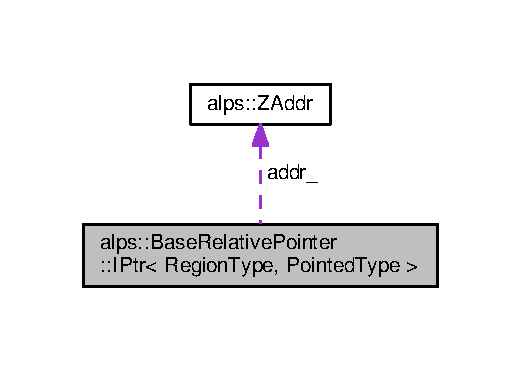
\includegraphics[width=250pt]{classalps_1_1BaseRelativePointer_1_1IPtr__coll__graph}
\end{center}
\end{figure}
\subsection*{Public Member Functions}
\begin{DoxyCompactItemize}
\item 
{\bfseries I\+Ptr} (Pointed\+Type $\ast$from)\hypertarget{classalps_1_1BaseRelativePointer_1_1IPtr_af35c8eb7b06b7b67dca454b36dd3cfe7}{}\label{classalps_1_1BaseRelativePointer_1_1IPtr_af35c8eb7b06b7b67dca454b36dd3cfe7}

\item 
{\bfseries I\+Ptr} (Region\+Type $\ast$pregion, Linear\+Addr offset)\hypertarget{classalps_1_1BaseRelativePointer_1_1IPtr_a9dae302ad3f661f80368a50609d32e2f}{}\label{classalps_1_1BaseRelativePointer_1_1IPtr_a9dae302ad3f661f80368a50609d32e2f}

\end{DoxyCompactItemize}
\subsection*{Public Attributes}
\begin{DoxyCompactItemize}
\item 
Region\+Type $\ast$ {\bfseries region\+\_\+}\hypertarget{classalps_1_1BaseRelativePointer_1_1IPtr_afa52ffae9a98b4ca95f89295db3634a6}{}\label{classalps_1_1BaseRelativePointer_1_1IPtr_afa52ffae9a98b4ca95f89295db3634a6}

\item 
\hyperlink{structalps_1_1ZAddr}{Z\+Addr} {\bfseries addr\+\_\+}\hypertarget{classalps_1_1BaseRelativePointer_1_1IPtr_a49c9c3ea7e1f7f289ed6b2c1ffd2912b}{}\label{classalps_1_1BaseRelativePointer_1_1IPtr_a49c9c3ea7e1f7f289ed6b2c1ffd2912b}

\end{DoxyCompactItemize}


\subsection{Detailed Description}
\subsubsection*{template$<$typename Region\+Type, typename Pointed\+Type$>$\\*
class alps\+::\+Base\+Relative\+Pointer\+::\+I\+Ptr$<$ Region\+Type, Pointed\+Type $>$}

Not a full-\/fledged smart pointer but rather an intermediate representation that simplifies cross-\/assignment between transient and persistent pointers. 

The documentation for this class was generated from the following file\+:\begin{DoxyCompactItemize}
\item 
/home/yuan/\+Benchmarks/whisper/mnemosyne-\/gcc/usermode/library/pmalloc/include/alps/include/alps/pegasus/pointer.\+hh\end{DoxyCompactItemize}

\hypertarget{structalps_1_1LfsOptions}{}\section{alps\+:\+:Lfs\+Options Struct Reference}
\label{structalps_1_1LfsOptions}\index{alps\+::\+Lfs\+Options@{alps\+::\+Lfs\+Options}}


Inheritance diagram for alps\+:\+:Lfs\+Options\+:
\nopagebreak
\begin{figure}[H]
\begin{center}
\leavevmode
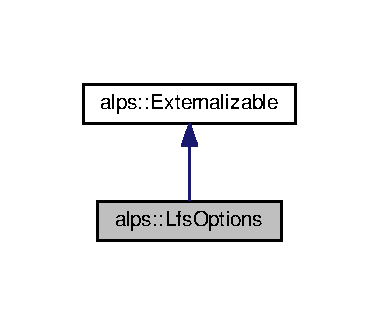
\includegraphics[width=182pt]{structalps_1_1LfsOptions__inherit__graph}
\end{center}
\end{figure}


Collaboration diagram for alps\+:\+:Lfs\+Options\+:
\nopagebreak
\begin{figure}[H]
\begin{center}
\leavevmode
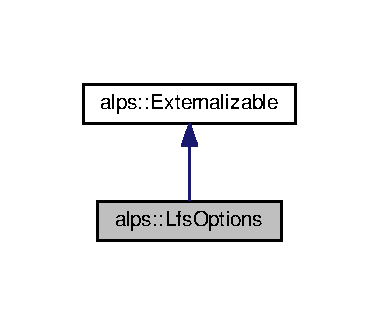
\includegraphics[width=182pt]{structalps_1_1LfsOptions__coll__graph}
\end{center}
\end{figure}
\subsection*{Public Member Functions}
\begin{DoxyCompactItemize}
\item 
\hyperlink{structalps_1_1LfsOptions_af7489183e0149dbf8a9fa7e827f49c60}{Lfs\+Options} ()
\end{DoxyCompactItemize}
\subsection*{Public Attributes}
\begin{DoxyCompactItemize}
\item 
unsigned int {\bfseries k\+Default\+Node} = 1\hypertarget{structalps_1_1LfsOptions_aaf7557c460b91aa0e95f65e278835cf9}{}\label{structalps_1_1LfsOptions_aaf7557c460b91aa0e95f65e278835cf9}

\item 
unsigned int {\bfseries k\+Default\+Node\+Count} = 1\hypertarget{structalps_1_1LfsOptions_a7140a100f93b6d6fadfbb862c68d7236}{}\label{structalps_1_1LfsOptions_a7140a100f93b6d6fadfbb862c68d7236}

\item 
size\+\_\+t {\bfseries k\+Default\+Book\+Size\+Bytes} = 8$\ast$1024\+L\+L\+U$\ast$1024\+L\+L\+U$\ast$1024\+L\+LU\hypertarget{structalps_1_1LfsOptions_a9675c2acbb53dc6bd54b204e05d17208}{}\label{structalps_1_1LfsOptions_a9675c2acbb53dc6bd54b204e05d17208}

\item 
unsigned int \hyperlink{structalps_1_1LfsOptions_ac08ad865ec69ce34c96e13f8de1c105e}{node}\hypertarget{structalps_1_1LfsOptions_ac08ad865ec69ce34c96e13f8de1c105e}{}\label{structalps_1_1LfsOptions_ac08ad865ec69ce34c96e13f8de1c105e}

\begin{DoxyCompactList}\small\item\em the current node I am running on \end{DoxyCompactList}\item 
unsigned int \hyperlink{structalps_1_1LfsOptions_a4961c4b5c1497f9d4e740b7ceed168d5}{node\+\_\+count}\hypertarget{structalps_1_1LfsOptions_a4961c4b5c1497f9d4e740b7ceed168d5}{}\label{structalps_1_1LfsOptions_a4961c4b5c1497f9d4e740b7ceed168d5}

\begin{DoxyCompactList}\small\item\em total number of nodes \end{DoxyCompactList}\item 
size\+\_\+t \hyperlink{structalps_1_1LfsOptions_ae8fd697e267bf399031e91b6aa0917b1}{book\+\_\+size\+\_\+bytes}\hypertarget{structalps_1_1LfsOptions_ae8fd697e267bf399031e91b6aa0917b1}{}\label{structalps_1_1LfsOptions_ae8fd697e267bf399031e91b6aa0917b1}

\begin{DoxyCompactList}\small\item\em book size \end{DoxyCompactList}\end{DoxyCompactItemize}
\subsection*{Additional Inherited Members}


\subsection{Constructor \& Destructor Documentation}
\index{alps\+::\+Lfs\+Options@{alps\+::\+Lfs\+Options}!Lfs\+Options@{Lfs\+Options}}
\index{Lfs\+Options@{Lfs\+Options}!alps\+::\+Lfs\+Options@{alps\+::\+Lfs\+Options}}
\subsubsection[{\texorpdfstring{Lfs\+Options()}{LfsOptions()}}]{\setlength{\rightskip}{0pt plus 5cm}alps\+::\+Lfs\+Options\+::\+Lfs\+Options (
\begin{DoxyParamCaption}
{}
\end{DoxyParamCaption}
)\hspace{0.3cm}{\ttfamily [inline]}}\hypertarget{structalps_1_1LfsOptions_af7489183e0149dbf8a9fa7e827f49c60}{}\label{structalps_1_1LfsOptions_af7489183e0149dbf8a9fa7e827f49c60}
Constructs option values with default values 

The documentation for this struct was generated from the following file\+:\begin{DoxyCompactItemize}
\item 
/home/yuan/\+Benchmarks/whisper/mnemosyne-\/gcc/usermode/library/pmalloc/include/alps/include/alps/pegasus/lfs\+\_\+options.\+hh\end{DoxyCompactItemize}

\hypertarget{classalps_1_1LfsRegionFile}{}\section{alps\+:\+:Lfs\+Region\+File Class Reference}
\label{classalps_1_1LfsRegionFile}\index{alps\+::\+Lfs\+Region\+File@{alps\+::\+Lfs\+Region\+File}}


Represents a region file backed by the Librarian FS.  




{\ttfamily \#include $<$lfs\+\_\+region\+\_\+file.\+hh$>$}



Inheritance diagram for alps\+:\+:Lfs\+Region\+File\+:
\nopagebreak
\begin{figure}[H]
\begin{center}
\leavevmode
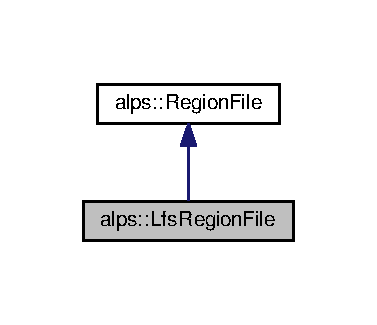
\includegraphics[width=181pt]{classalps_1_1LfsRegionFile__inherit__graph}
\end{center}
\end{figure}


Collaboration diagram for alps\+:\+:Lfs\+Region\+File\+:
\nopagebreak
\begin{figure}[H]
\begin{center}
\leavevmode
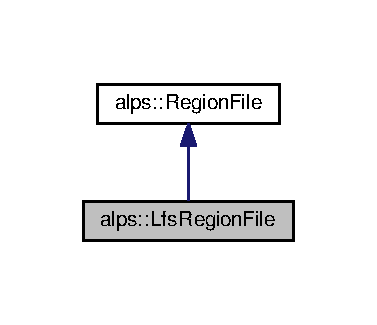
\includegraphics[width=181pt]{classalps_1_1LfsRegionFile__coll__graph}
\end{center}
\end{figure}
\subsection*{Public Types}
\begin{DoxyCompactItemize}
\item 
enum {\bfseries Interleave\+Policy} \{ {\bfseries k\+Precise\+Allocate} = 0, 
{\bfseries k\+Round\+Robin}
 \}\hypertarget{classalps_1_1LfsRegionFile_a680a5b2fdfe08e752b30ae155901d118}{}\label{classalps_1_1LfsRegionFile_a680a5b2fdfe08e752b30ae155901d118}

\end{DoxyCompactItemize}
\subsection*{Public Member Functions}
\begin{DoxyCompactItemize}
\item 
{\bfseries Lfs\+Region\+File} (const boost\+::filesystem\+::path \&pathname, const \hyperlink{structalps_1_1PegasusOptions}{Pegasus\+Options} \&pegasus\+\_\+options)\hypertarget{classalps_1_1LfsRegionFile_a81c1bef03c892fe27b3c436d541aa164}{}\label{classalps_1_1LfsRegionFile_a81c1bef03c892fe27b3c436d541aa164}

\item 
\hyperlink{group__ERRORCODES_ga6263a3c9a0b8d36aea21cdd835ac99fe}{Error\+Code} {\bfseries create} (mode\+\_\+t mode)\hypertarget{classalps_1_1LfsRegionFile_aec4c0a975a453de5a92313a15febd797}{}\label{classalps_1_1LfsRegionFile_aec4c0a975a453de5a92313a15febd797}

\item 
\hyperlink{group__ERRORCODES_ga6263a3c9a0b8d36aea21cdd835ac99fe}{Error\+Code} {\bfseries open} (int flags, mode\+\_\+t mode)\hypertarget{classalps_1_1LfsRegionFile_a40ed4ec47a3f8f294026c2599e0878f7}{}\label{classalps_1_1LfsRegionFile_a40ed4ec47a3f8f294026c2599e0878f7}

\item 
\hyperlink{group__ERRORCODES_ga6263a3c9a0b8d36aea21cdd835ac99fe}{Error\+Code} {\bfseries open} (int flags)\hypertarget{classalps_1_1LfsRegionFile_a97048d3ee58fc7e2fb107dd7fa75c97d}{}\label{classalps_1_1LfsRegionFile_a97048d3ee58fc7e2fb107dd7fa75c97d}

\item 
\hyperlink{group__ERRORCODES_ga6263a3c9a0b8d36aea21cdd835ac99fe}{Error\+Code} {\bfseries unlink} ()\hypertarget{classalps_1_1LfsRegionFile_ac31fc14d0caf4b6448478032b859907c}{}\label{classalps_1_1LfsRegionFile_ac31fc14d0caf4b6448478032b859907c}

\item 
\hyperlink{group__ERRORCODES_ga6263a3c9a0b8d36aea21cdd835ac99fe}{Error\+Code} {\bfseries close} ()\hypertarget{classalps_1_1LfsRegionFile_aafbc14718eaf10a372a7f7e1ce980cc0}{}\label{classalps_1_1LfsRegionFile_aafbc14718eaf10a372a7f7e1ce980cc0}

\item 
\hyperlink{group__ERRORCODES_ga6263a3c9a0b8d36aea21cdd835ac99fe}{Error\+Code} {\bfseries truncate} (loff\+\_\+t length)\hypertarget{classalps_1_1LfsRegionFile_ae6b7e891a39e1fe2b35a3301a94e89f0}{}\label{classalps_1_1LfsRegionFile_ae6b7e891a39e1fe2b35a3301a94e89f0}

\item 
\hyperlink{group__ERRORCODES_ga6263a3c9a0b8d36aea21cdd835ac99fe}{Error\+Code} {\bfseries size} (loff\+\_\+t $\ast$length)\hypertarget{classalps_1_1LfsRegionFile_a0e243bd2818afb0074c8b081ef832244}{}\label{classalps_1_1LfsRegionFile_a0e243bd2818afb0074c8b081ef832244}

\item 
\hyperlink{group__ERRORCODES_ga6263a3c9a0b8d36aea21cdd835ac99fe}{Error\+Code} {\bfseries map} (void $\ast$addr\+\_\+hint, size\+\_\+t length, int prot, int flags, loff\+\_\+t offset, void $\ast$$\ast$mapped\+\_\+addr)\hypertarget{classalps_1_1LfsRegionFile_a0422a2e6993d2f9514f8b9d3f8591393}{}\label{classalps_1_1LfsRegionFile_a0422a2e6993d2f9514f8b9d3f8591393}

\item 
\hyperlink{group__ERRORCODES_ga6263a3c9a0b8d36aea21cdd835ac99fe}{Error\+Code} {\bfseries unmap} (void $\ast$addr, size\+\_\+t length)\hypertarget{classalps_1_1LfsRegionFile_a45abfa040991646add32d5cfd032736a}{}\label{classalps_1_1LfsRegionFile_a45abfa040991646add32d5cfd032736a}

\item 
\hyperlink{group__ERRORCODES_ga6263a3c9a0b8d36aea21cdd835ac99fe}{Error\+Code} {\bfseries getxattr} (const char $\ast$name, void $\ast$value, size\+\_\+t size)\hypertarget{classalps_1_1LfsRegionFile_ae6fc356df22d6ec82d97e35019013bdc}{}\label{classalps_1_1LfsRegionFile_ae6fc356df22d6ec82d97e35019013bdc}

\item 
\hyperlink{group__ERRORCODES_ga6263a3c9a0b8d36aea21cdd835ac99fe}{Error\+Code} {\bfseries setxattr} (const char $\ast$name, const void $\ast$value, size\+\_\+t size, int flags)\hypertarget{classalps_1_1LfsRegionFile_ab3e7f8d216d341d4157444c2a5ae7625}{}\label{classalps_1_1LfsRegionFile_ab3e7f8d216d341d4157444c2a5ae7625}

\item 
size\+\_\+t {\bfseries booksize} ()\hypertarget{classalps_1_1LfsRegionFile_a526610896c98d23ddd9e29fbe20c04a6}{}\label{classalps_1_1LfsRegionFile_a526610896c98d23ddd9e29fbe20c04a6}

\end{DoxyCompactItemize}
\subsection*{Static Public Member Functions}
\begin{DoxyCompactItemize}
\item 
static \hyperlink{classalps_1_1RegionFile}{Region\+File} $\ast$ {\bfseries construct} (const boost\+::filesystem\+::path \&pathname, const \hyperlink{structalps_1_1PegasusOptions}{Pegasus\+Options} \&pegasus\+\_\+options)\hypertarget{classalps_1_1LfsRegionFile_a0137dec1c0ab38afd0d58c2433b20ab1}{}\label{classalps_1_1LfsRegionFile_a0137dec1c0ab38afd0d58c2433b20ab1}

\end{DoxyCompactItemize}
\subsection*{Static Public Attributes}
\begin{DoxyCompactItemize}
\item 
static Interleave\+Policy {\bfseries interleave\+\_\+policy\+\_\+}\hypertarget{classalps_1_1LfsRegionFile_a1dbc8a71fb39f79ea0884ccf80495bfb}{}\label{classalps_1_1LfsRegionFile_a1dbc8a71fb39f79ea0884ccf80495bfb}

\end{DoxyCompactItemize}


The documentation for this class was generated from the following files\+:\begin{DoxyCompactItemize}
\item 
/home/yuan/\+Benchmarks/whisper/mnemosyne-\/gcc/usermode/library/pmalloc/include/alps/src/pegasus/lfs\+\_\+region\+\_\+file.\+hh\item 
/home/yuan/\+Benchmarks/whisper/mnemosyne-\/gcc/usermode/library/pmalloc/include/alps/src/pegasus/lfs\+\_\+region\+\_\+file.\+cc\end{DoxyCompactItemize}

\hypertarget{classalps_1_1LfsTopology}{}\section{alps\+:\+:Lfs\+Topology Class Reference}
\label{classalps_1_1LfsTopology}\index{alps\+::\+Lfs\+Topology@{alps\+::\+Lfs\+Topology}}


Inheritance diagram for alps\+:\+:Lfs\+Topology\+:
\nopagebreak
\begin{figure}[H]
\begin{center}
\leavevmode
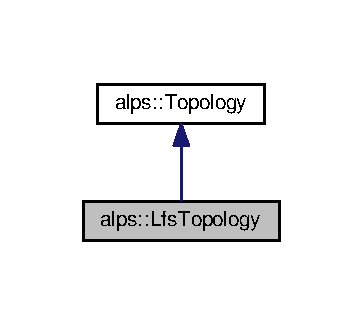
\includegraphics[width=174pt]{classalps_1_1LfsTopology__inherit__graph}
\end{center}
\end{figure}


Collaboration diagram for alps\+:\+:Lfs\+Topology\+:
\nopagebreak
\begin{figure}[H]
\begin{center}
\leavevmode
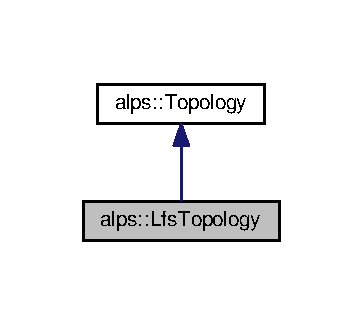
\includegraphics[width=174pt]{classalps_1_1LfsTopology__coll__graph}
\end{center}
\end{figure}
\subsection*{Public Member Functions}
\begin{DoxyCompactItemize}
\item 
{\bfseries Lfs\+Topology} (const boost\+::filesystem\+::path \&path, const \hyperlink{structalps_1_1PegasusOptions}{Pegasus\+Options} \&pegasus\+\_\+options)\hypertarget{classalps_1_1LfsTopology_a53842f5efcd733fae7e582becbcde3f7}{}\label{classalps_1_1LfsTopology_a53842f5efcd733fae7e582becbcde3f7}

\item 
Interleave\+Group \hyperlink{classalps_1_1LfsTopology_a1c6476bae1c7aa63b9f36a9369d6b23f}{max\+\_\+interleave\+\_\+group} ()\hypertarget{classalps_1_1LfsTopology_a1c6476bae1c7aa63b9f36a9369d6b23f}{}\label{classalps_1_1LfsTopology_a1c6476bae1c7aa63b9f36a9369d6b23f}

\begin{DoxyCompactList}\small\item\em Returns the highest node number available in the system. \end{DoxyCompactList}\item 
Interleave\+Group \hyperlink{classalps_1_1LfsTopology_a5b3e607fc2273159b70f7278d43d5029}{nearest\+\_\+ig} ()\hypertarget{classalps_1_1LfsTopology_a5b3e607fc2273159b70f7278d43d5029}{}\label{classalps_1_1LfsTopology_a5b3e607fc2273159b70f7278d43d5029}

\begin{DoxyCompactList}\small\item\em Returns the nearest interleave group to the node the calling process is running on. \end{DoxyCompactList}\end{DoxyCompactItemize}
\subsection*{Static Public Member Functions}
\begin{DoxyCompactItemize}
\item 
static \hyperlink{classalps_1_1Topology}{Topology} $\ast$ {\bfseries construct} (const boost\+::filesystem\+::path \&pathname, const \hyperlink{structalps_1_1PegasusOptions}{Pegasus\+Options} \&pegasus\+\_\+options)\hypertarget{classalps_1_1LfsTopology_ae753f28a0cb3510278423386d83e2d14}{}\label{classalps_1_1LfsTopology_ae753f28a0cb3510278423386d83e2d14}

\end{DoxyCompactItemize}


The documentation for this class was generated from the following files\+:\begin{DoxyCompactItemize}
\item 
/home/yuan/\+Benchmarks/whisper/mnemosyne-\/gcc/usermode/library/pmalloc/include/alps/src/pegasus/lfs\+\_\+topology.\+hh\item 
/home/yuan/\+Benchmarks/whisper/mnemosyne-\/gcc/usermode/library/pmalloc/include/alps/src/pegasus/lfs\+\_\+topology.\+cc\end{DoxyCompactItemize}

\hypertarget{structalps_1_1BacktraceContext_1_1LibBacktraceInfo}{}\section{alps\+:\+:Backtrace\+Context\+:\+:Lib\+Backtrace\+Info Struct Reference}
\label{structalps_1_1BacktraceContext_1_1LibBacktraceInfo}\index{alps\+::\+Backtrace\+Context\+::\+Lib\+Backtrace\+Info@{alps\+::\+Backtrace\+Context\+::\+Lib\+Backtrace\+Info}}
\subsection*{Public Attributes}
\begin{DoxyCompactItemize}
\item 
uintptr\+\_\+t {\bfseries address\+\_\+}\hypertarget{structalps_1_1BacktraceContext_1_1LibBacktraceInfo_a6f081350503486bc958cfa0678f6259b}{}\label{structalps_1_1BacktraceContext_1_1LibBacktraceInfo_a6f081350503486bc958cfa0678f6259b}

\item 
std\+::string {\bfseries srcfile\+\_\+}\hypertarget{structalps_1_1BacktraceContext_1_1LibBacktraceInfo_a40f51d259e2e2bb91d42b485caf054e3}{}\label{structalps_1_1BacktraceContext_1_1LibBacktraceInfo_a40f51d259e2e2bb91d42b485caf054e3}

\item 
int {\bfseries srclineno\+\_\+}\hypertarget{structalps_1_1BacktraceContext_1_1LibBacktraceInfo_a79b52c6cbb725765a7ff1a5b0922a684}{}\label{structalps_1_1BacktraceContext_1_1LibBacktraceInfo_a79b52c6cbb725765a7ff1a5b0922a684}

\item 
std\+::string {\bfseries function\+\_\+}\hypertarget{structalps_1_1BacktraceContext_1_1LibBacktraceInfo_a60af9337a0b07c3d79c931ca66232b9d}{}\label{structalps_1_1BacktraceContext_1_1LibBacktraceInfo_a60af9337a0b07c3d79c931ca66232b9d}

\end{DoxyCompactItemize}


The documentation for this struct was generated from the following file\+:\begin{DoxyCompactItemize}
\item 
/home/yuan/\+Benchmarks/whisper/mnemosyne-\/gcc/usermode/library/pmalloc/include/alps/src/common/rich\+\_\+backtrace.\+cc\end{DoxyCompactItemize}

\hypertarget{classalps_1_1Mappable}{}\section{alps\+:\+:Mappable$<$ Region\+Type, Memory\+Map\+Impl, Pointer\+Impl $>$ Class Template Reference}
\label{classalps_1_1Mappable}\index{alps\+::\+Mappable$<$ Region\+Type, Memory\+Map\+Impl, Pointer\+Impl $>$@{alps\+::\+Mappable$<$ Region\+Type, Memory\+Map\+Impl, Pointer\+Impl $>$}}


A template mixin class for defining mappable region types.  




{\ttfamily \#include $<$mappable.\+hh$>$}



Inheritance diagram for alps\+:\+:Mappable$<$ Region\+Type, Memory\+Map\+Impl, Pointer\+Impl $>$\+:
\nopagebreak
\begin{figure}[H]
\begin{center}
\leavevmode
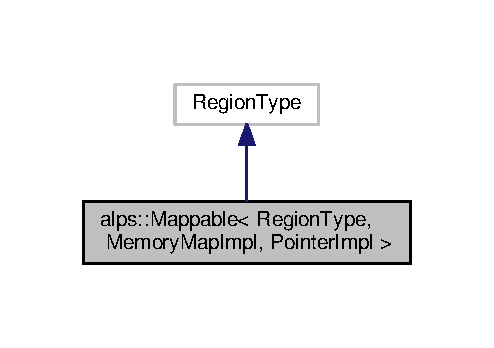
\includegraphics[width=237pt]{classalps_1_1Mappable__inherit__graph}
\end{center}
\end{figure}


Collaboration diagram for alps\+:\+:Mappable$<$ Region\+Type, Memory\+Map\+Impl, Pointer\+Impl $>$\+:
\nopagebreak
\begin{figure}[H]
\begin{center}
\leavevmode
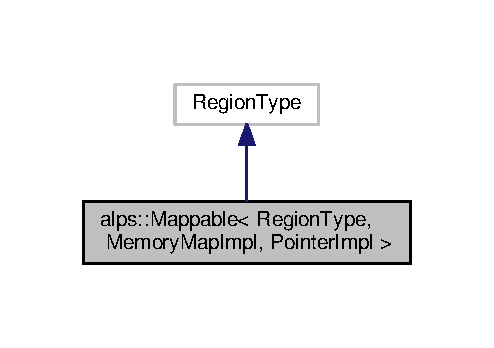
\includegraphics[width=237pt]{classalps_1_1Mappable__coll__graph}
\end{center}
\end{figure}
\subsection*{Public Types}
\begin{DoxyCompactItemize}
\item 
{\footnotesize template$<$class T $>$ }\\using {\bfseries T\+Ptr} = typename Pointer\+Impl\+::template T\+Ptr$<$ \hyperlink{classalps_1_1Mappable}{Mappable}, T $>$\hypertarget{classalps_1_1Mappable_acaa8e7c54b38126cd6c25c5ed26fbe87}{}\label{classalps_1_1Mappable_acaa8e7c54b38126cd6c25c5ed26fbe87}

\item 
{\footnotesize template$<$class T $>$ }\\using {\bfseries P\+Ptr} = typename Pointer\+Impl\+::template P\+Ptr$<$ \hyperlink{classalps_1_1Mappable}{Mappable}, T $>$\hypertarget{classalps_1_1Mappable_ac29c1a848f5fae659e2f03296ddc4e8a}{}\label{classalps_1_1Mappable_ac29c1a848f5fae659e2f03296ddc4e8a}

\item 
{\footnotesize template$<$class T $>$ }\\using {\bfseries Z\+Ptr} = typename Pointer\+Impl\+::template Z\+Ptr$<$ \hyperlink{classalps_1_1Mappable}{Mappable}, T $>$\hypertarget{classalps_1_1Mappable_ace436b9205b93077e8b4696b394ccc97}{}\label{classalps_1_1Mappable_ace436b9205b93077e8b4696b394ccc97}

\end{DoxyCompactItemize}
\subsection*{Public Member Functions}
\begin{DoxyCompactItemize}
\item 
{\bfseries Mappable} (\hyperlink{classalps_1_1AddressSpace}{Address\+Space} $\ast$address\+\_\+space, \hyperlink{classalps_1_1RegionFile}{Region\+File} $\ast$file)\hypertarget{classalps_1_1Mappable_a0dd4c0bbb33fd9268b8459b184440705}{}\label{classalps_1_1Mappable_a0dd4c0bbb33fd9268b8459b184440705}

\item 
\hyperlink{group__ERRORCODES_ga6263a3c9a0b8d36aea21cdd835ac99fe}{Error\+Code} {\bfseries map} ()\hypertarget{classalps_1_1Mappable_a5ae691f7e71cac7cc58155703ef4a5ac}{}\label{classalps_1_1Mappable_a5ae691f7e71cac7cc58155703ef4a5ac}

\item 
\hyperlink{group__ERRORCODES_ga6263a3c9a0b8d36aea21cdd835ac99fe}{Error\+Code} {\bfseries unmap} ()\hypertarget{classalps_1_1Mappable_a8394bd3c972b7c8d4c98604d71217f25}{}\label{classalps_1_1Mappable_a8394bd3c972b7c8d4c98604d71217f25}

\item 
{\footnotesize template$<$class T $>$ }\\T\+Ptr$<$ T $>$ {\bfseries base} (Linear\+Addr offset)\hypertarget{classalps_1_1Mappable_abe9367121a591f7b8a351a8a808bd838}{}\label{classalps_1_1Mappable_abe9367121a591f7b8a351a8a808bd838}

\item 
uintptr\+\_\+t {\bfseries trans} (Linear\+Addr offset)\hypertarget{classalps_1_1Mappable_a3a022abb4190c60948d60bece0188c48}{}\label{classalps_1_1Mappable_a3a022abb4190c60948d60bece0188c48}

\end{DoxyCompactItemize}
\subsection*{Friends}
\begin{DoxyCompactItemize}
\item 
class {\bfseries Address\+Space}\hypertarget{classalps_1_1Mappable_a4c0de12c4816e1f285ed094ad8c7f9c8}{}\label{classalps_1_1Mappable_a4c0de12c4816e1f285ed094ad8c7f9c8}

\end{DoxyCompactItemize}


\subsection{Detailed Description}
\subsubsection*{template$<$class Region\+Type, class Memory\+Map\+Impl, class Pointer\+Impl$>$\\*
class alps\+::\+Mappable$<$ Region\+Type, Memory\+Map\+Impl, Pointer\+Impl $>$}

The Memory\+Map\+Impl class defines the mapping policy that implements mapping of the underlying region file(s) onto the logical address space.

The Pointer\+Impl class defines smart pointer types for naming (addressing) and referencing locations within the region.

There is no notion of a root pointer baked into the A\+PI. However, users may agree on a convention where offset 0x0 represents a root, and instantiate a smart pointer that points to offset 0x0 and use that as a root pointer. 

The documentation for this class was generated from the following file\+:\begin{DoxyCompactItemize}
\item 
/home/yuan/\+Benchmarks/whisper/mnemosyne-\/gcc/usermode/library/pmalloc/include/alps/include/alps/pegasus/mappable.\+hh\end{DoxyCompactItemize}

\hypertarget{classalps_1_1MemoryManager}{}\section{alps\+:\+:Memory\+Manager Class Reference}
\label{classalps_1_1MemoryManager}\index{alps\+::\+Memory\+Manager@{alps\+::\+Memory\+Manager}}


The memory manager provides a mechanism for directly mapping persistent region files to virtual memory regions.  




{\ttfamily \#include $<$mm.\+hh$>$}

\subsection*{Public Member Functions}
\begin{DoxyCompactItemize}
\item 
\hyperlink{group__ERRORCODES_ga6263a3c9a0b8d36aea21cdd835ac99fe}{Error\+Code} {\bfseries map} (\hyperlink{classalps_1_1Region}{Region} $\ast$region, off\+\_\+t offset, size\+\_\+t length, void $\ast$addr\+\_\+hint, int prot, int flags, \hyperlink{classalps_1_1VmArea}{Vm\+Area} $\ast$$\ast$vmarea)\hypertarget{classalps_1_1MemoryManager_a0795e8c13ff24a1fd717fac961f9c797}{}\label{classalps_1_1MemoryManager_a0795e8c13ff24a1fd717fac961f9c797}

\item 
\hyperlink{group__ERRORCODES_ga6263a3c9a0b8d36aea21cdd835ac99fe}{Error\+Code} {\bfseries unmap} (\hyperlink{classalps_1_1Region}{Region} $\ast$region, void $\ast$addr, size\+\_\+t length)\hypertarget{classalps_1_1MemoryManager_a7f9e8c4d40c4a2a6417de4fad89f8d46}{}\label{classalps_1_1MemoryManager_a7f9e8c4d40c4a2a6417de4fad89f8d46}

\item 
\hyperlink{group__ERRORCODES_ga6263a3c9a0b8d36aea21cdd835ac99fe}{Error\+Code} {\bfseries rtrans} (void $\ast$addr, \hyperlink{classalps_1_1Region}{Region} $\ast$$\ast$pregion, Linear\+Addr $\ast$offset)\hypertarget{classalps_1_1MemoryManager_ad436265484fce31b03e714f031f28403}{}\label{classalps_1_1MemoryManager_ad436265484fce31b03e714f031f28403}

\item 
\hyperlink{group__ERRORCODES_ga6263a3c9a0b8d36aea21cdd835ac99fe}{Error\+Code} {\bfseries rtrans} (uintptr\+\_\+t addr, \hyperlink{classalps_1_1Region}{Region} $\ast$$\ast$pregion, Linear\+Addr $\ast$offset)\hypertarget{classalps_1_1MemoryManager_a5f27ecadfe7b172003cdecca423ee56c}{}\label{classalps_1_1MemoryManager_a5f27ecadfe7b172003cdecca423ee56c}

\end{DoxyCompactItemize}


\subsection{Detailed Description}
The manager is intended for use by a per-\/region memory mapper (Memory\+Map) that implements mapping policy.

\begin{DoxyRefDesc}{Todo}
\item[\hyperlink{todo__todo000001}{Todo}]Provide an A\+PI for picking address hints\+:
\begin{DoxyItemize}
\item best effort mapping\+: find the largest hole in the address space where we can map regions this can guide segment map to pick the right segment size
\item guide underlying OS by picking an address\+\_\+hint based on our past knowledge about persistent regions to minimize address space fragmentation similar to the Mnemosyne runtime (this could be implemented in the map method) 
\end{DoxyItemize}\end{DoxyRefDesc}


The documentation for this class was generated from the following files\+:\begin{DoxyCompactItemize}
\item 
/home/yuan/\+Benchmarks/whisper/mnemosyne-\/gcc/usermode/library/pmalloc/include/alps/src/pegasus/mm.\+hh\item 
/home/yuan/\+Benchmarks/whisper/mnemosyne-\/gcc/usermode/library/pmalloc/include/alps/src/pegasus/mm.\+cc\end{DoxyCompactItemize}

\hypertarget{classalps_1_1MultiRegionFile}{}\section{alps\+:\+:Multi\+Region\+File Class Reference}
\label{classalps_1_1MultiRegionFile}\index{alps\+::\+Multi\+Region\+File@{alps\+::\+Multi\+Region\+File}}


Represents a pseudo region file comprising multiple region files.  




{\ttfamily \#include $<$multi\+\_\+region\+\_\+file.\+hh$>$}



Inheritance diagram for alps\+:\+:Multi\+Region\+File\+:
\nopagebreak
\begin{figure}[H]
\begin{center}
\leavevmode
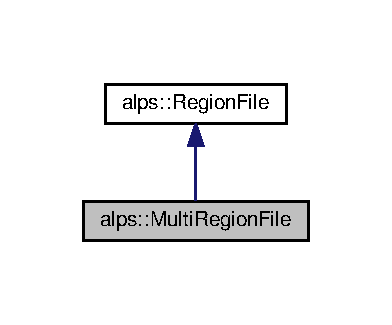
\includegraphics[width=188pt]{classalps_1_1MultiRegionFile__inherit__graph}
\end{center}
\end{figure}


Collaboration diagram for alps\+:\+:Multi\+Region\+File\+:
\nopagebreak
\begin{figure}[H]
\begin{center}
\leavevmode
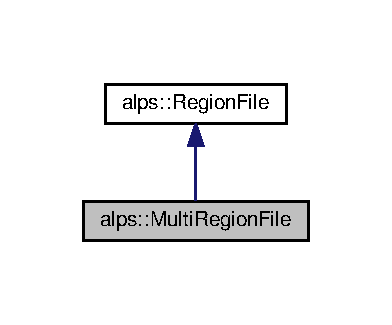
\includegraphics[width=188pt]{classalps_1_1MultiRegionFile__coll__graph}
\end{center}
\end{figure}
\subsection*{Public Member Functions}
\begin{DoxyCompactItemize}
\item 
{\bfseries Multi\+Region\+File} (const std\+::vector$<$ \hyperlink{classalps_1_1RegionFile}{Region\+File} $\ast$ $>$ region\+\_\+files)\hypertarget{classalps_1_1MultiRegionFile_ae4e25dd6261d7a1745a2e355c14ed11e}{}\label{classalps_1_1MultiRegionFile_ae4e25dd6261d7a1745a2e355c14ed11e}

\item 
\hyperlink{group__ERRORCODES_ga6263a3c9a0b8d36aea21cdd835ac99fe}{Error\+Code} \hyperlink{classalps_1_1MultiRegionFile_a914948b93698e5bf84792f793a2c6df0}{create} (mode\+\_\+t mode)\hypertarget{classalps_1_1MultiRegionFile_a914948b93698e5bf84792f793a2c6df0}{}\label{classalps_1_1MultiRegionFile_a914948b93698e5bf84792f793a2c6df0}

\begin{DoxyCompactList}\small\item\em Operation not supported for this region file type. \end{DoxyCompactList}\item 
\hyperlink{group__ERRORCODES_ga6263a3c9a0b8d36aea21cdd835ac99fe}{Error\+Code} {\bfseries open} (int flags, mode\+\_\+t mode)\hypertarget{classalps_1_1MultiRegionFile_ada71637b82174b46b183fbae8587734e}{}\label{classalps_1_1MultiRegionFile_ada71637b82174b46b183fbae8587734e}

\item 
\hyperlink{group__ERRORCODES_ga6263a3c9a0b8d36aea21cdd835ac99fe}{Error\+Code} {\bfseries open} (int flags)\hypertarget{classalps_1_1MultiRegionFile_a2fb08745a10e08b8a3428396761cf9ff}{}\label{classalps_1_1MultiRegionFile_a2fb08745a10e08b8a3428396761cf9ff}

\item 
\hyperlink{group__ERRORCODES_ga6263a3c9a0b8d36aea21cdd835ac99fe}{Error\+Code} \hyperlink{classalps_1_1MultiRegionFile_ac3b66aae57953f47d15618d4a6f9f4bf}{unlink} ()\hypertarget{classalps_1_1MultiRegionFile_ac3b66aae57953f47d15618d4a6f9f4bf}{}\label{classalps_1_1MultiRegionFile_ac3b66aae57953f47d15618d4a6f9f4bf}

\begin{DoxyCompactList}\small\item\em Operation not supported for this region file type. \end{DoxyCompactList}\item 
\hyperlink{group__ERRORCODES_ga6263a3c9a0b8d36aea21cdd835ac99fe}{Error\+Code} {\bfseries close} ()\hypertarget{classalps_1_1MultiRegionFile_a9fe28ebb5704731c642fe2203648016a}{}\label{classalps_1_1MultiRegionFile_a9fe28ebb5704731c642fe2203648016a}

\item 
\hyperlink{group__ERRORCODES_ga6263a3c9a0b8d36aea21cdd835ac99fe}{Error\+Code} \hyperlink{classalps_1_1MultiRegionFile_af330f12ef62f3a140130ef5c58370513}{truncate} (loff\+\_\+t length)\hypertarget{classalps_1_1MultiRegionFile_af330f12ef62f3a140130ef5c58370513}{}\label{classalps_1_1MultiRegionFile_af330f12ef62f3a140130ef5c58370513}

\begin{DoxyCompactList}\small\item\em Operation not supported for this region file type. \end{DoxyCompactList}\item 
\hyperlink{group__ERRORCODES_ga6263a3c9a0b8d36aea21cdd835ac99fe}{Error\+Code} {\bfseries size} (loff\+\_\+t $\ast$length)\hypertarget{classalps_1_1MultiRegionFile_a083ab071bc83e2f9e647e978d0afa0c1}{}\label{classalps_1_1MultiRegionFile_a083ab071bc83e2f9e647e978d0afa0c1}

\item 
\hyperlink{group__ERRORCODES_ga6263a3c9a0b8d36aea21cdd835ac99fe}{Error\+Code} {\bfseries map} (void $\ast$addr\+\_\+hint, size\+\_\+t length, int prot, int flags, loff\+\_\+t offset, void $\ast$$\ast$mapped\+\_\+addr)\hypertarget{classalps_1_1MultiRegionFile_adce5e1dde0d9b3b2f170f7c5d9cd2718}{}\label{classalps_1_1MultiRegionFile_adce5e1dde0d9b3b2f170f7c5d9cd2718}

\item 
\hyperlink{group__ERRORCODES_ga6263a3c9a0b8d36aea21cdd835ac99fe}{Error\+Code} {\bfseries unmap} (void $\ast$addr, size\+\_\+t length)\hypertarget{classalps_1_1MultiRegionFile_a0dedb7bee4b25f26f0f86bdf40dac35b}{}\label{classalps_1_1MultiRegionFile_a0dedb7bee4b25f26f0f86bdf40dac35b}

\item 
\hyperlink{group__ERRORCODES_ga6263a3c9a0b8d36aea21cdd835ac99fe}{Error\+Code} \hyperlink{classalps_1_1MultiRegionFile_ab1121b16b2a12746f87fb5c1af75ad52}{getxattr} (const char $\ast$name, void $\ast$value, size\+\_\+t size)\hypertarget{classalps_1_1MultiRegionFile_ab1121b16b2a12746f87fb5c1af75ad52}{}\label{classalps_1_1MultiRegionFile_ab1121b16b2a12746f87fb5c1af75ad52}

\begin{DoxyCompactList}\small\item\em Operation not supported for this region file type. \end{DoxyCompactList}\item 
\hyperlink{group__ERRORCODES_ga6263a3c9a0b8d36aea21cdd835ac99fe}{Error\+Code} \hyperlink{classalps_1_1MultiRegionFile_a610085fd92e3e5effb9ba6c872981831}{setxattr} (const char $\ast$name, const void $\ast$value, size\+\_\+t size, int flags)\hypertarget{classalps_1_1MultiRegionFile_a610085fd92e3e5effb9ba6c872981831}{}\label{classalps_1_1MultiRegionFile_a610085fd92e3e5effb9ba6c872981831}

\begin{DoxyCompactList}\small\item\em Operation not supported for this region file type. \end{DoxyCompactList}\item 
size\+\_\+t {\bfseries booksize} ()\hypertarget{classalps_1_1MultiRegionFile_a4140e32344954ef79c2dce39bf942a7d}{}\label{classalps_1_1MultiRegionFile_a4140e32344954ef79c2dce39bf942a7d}

\item 
\hyperlink{group__ERRORCODES_ga6263a3c9a0b8d36aea21cdd835ac99fe}{Error\+Code} {\bfseries set\+\_\+interleave\+\_\+group} (loff\+\_\+t offset, loff\+\_\+t length, const std\+::vector$<$ Interleave\+Group $>$ \&vig)\hypertarget{classalps_1_1MultiRegionFile_aa5d9db02bcb0450caf1df87fc45a09f7}{}\label{classalps_1_1MultiRegionFile_aa5d9db02bcb0450caf1df87fc45a09f7}

\item 
\hyperlink{group__ERRORCODES_ga6263a3c9a0b8d36aea21cdd835ac99fe}{Error\+Code} {\bfseries interleave\+\_\+group} (loff\+\_\+t offset, loff\+\_\+t length, std\+::vector$<$ Interleave\+Group $>$ $\ast$vig)\hypertarget{classalps_1_1MultiRegionFile_a9cbdd991f99da438edaf5c697f282f47}{}\label{classalps_1_1MultiRegionFile_a9cbdd991f99da438edaf5c697f282f47}

\end{DoxyCompactItemize}


\subsection{Detailed Description}
We provide this pseudo region file as a helper class for glueing and mapping multiple existing region files as a single contiguous file. This class does not support operations that require modifying file-\/system metadata of underlying region files, including create, truncate, unlink, set/get attributes. 

The documentation for this class was generated from the following files\+:\begin{DoxyCompactItemize}
\item 
/home/yuan/\+Benchmarks/whisper/mnemosyne-\/gcc/usermode/library/pmalloc/include/alps/src/pegasus/multi\+\_\+region\+\_\+file.\+hh\item 
/home/yuan/\+Benchmarks/whisper/mnemosyne-\/gcc/usermode/library/pmalloc/include/alps/src/pegasus/multi\+\_\+region\+\_\+file.\+cc\end{DoxyCompactItemize}

\hypertarget{structalps_1_1PAddr}{}\section{alps\+:\+:P\+Addr Struct Reference}
\label{structalps_1_1PAddr}\index{alps\+::\+P\+Addr@{alps\+::\+P\+Addr}}
\subsection*{Public Member Functions}
\begin{DoxyCompactItemize}
\item 
{\bfseries P\+Addr} (Linear\+Addr linear\+\_\+addr)\hypertarget{structalps_1_1PAddr_a8982be9f74d2315051a80e1caca63ed5}{}\label{structalps_1_1PAddr_a8982be9f74d2315051a80e1caca63ed5}

\item 
bool {\bfseries operator==} (const \hyperlink{structalps_1_1PAddr}{P\+Addr} \&other) const \hypertarget{structalps_1_1PAddr_a03b2b290453ddced8540cbff0fd3492f}{}\label{structalps_1_1PAddr_a03b2b290453ddced8540cbff0fd3492f}

\item 
bool {\bfseries operator!=} (const \hyperlink{structalps_1_1PAddr}{P\+Addr} \&other) const \hypertarget{structalps_1_1PAddr_a1afc56c34672ca32a62d81eed3be1fbb}{}\label{structalps_1_1PAddr_a1afc56c34672ca32a62d81eed3be1fbb}

\item 
void {\bfseries stream\+\_\+to} (std\+::ostream \&os) const \hypertarget{structalps_1_1PAddr_a9c0b6d407c42585d6061ea60cf163b3e}{}\label{structalps_1_1PAddr_a9c0b6d407c42585d6061ea60cf163b3e}

\end{DoxyCompactItemize}
\subsection*{Public Attributes}
\begin{DoxyCompactItemize}
\item 
Linear\+Addr {\bfseries linear\+\_\+addr\+\_\+}\hypertarget{structalps_1_1PAddr_ab0968857be1118d355e98c741838e7f9}{}\label{structalps_1_1PAddr_ab0968857be1118d355e98c741838e7f9}

\end{DoxyCompactItemize}


The documentation for this struct was generated from the following file\+:\begin{DoxyCompactItemize}
\item 
/home/yuan/\+Benchmarks/whisper/mnemosyne-\/gcc/usermode/library/pmalloc/include/alps/include/alps/pegasus/addr.\+hh\end{DoxyCompactItemize}

\hypertarget{classalps_1_1PegasThread}{}\section{alps\+:\+:Pegas\+Thread Class Reference}
\label{classalps_1_1PegasThread}\index{alps\+::\+Pegas\+Thread@{alps\+::\+Pegas\+Thread}}


Collaboration diagram for alps\+:\+:Pegas\+Thread\+:
\nopagebreak
\begin{figure}[H]
\begin{center}
\leavevmode
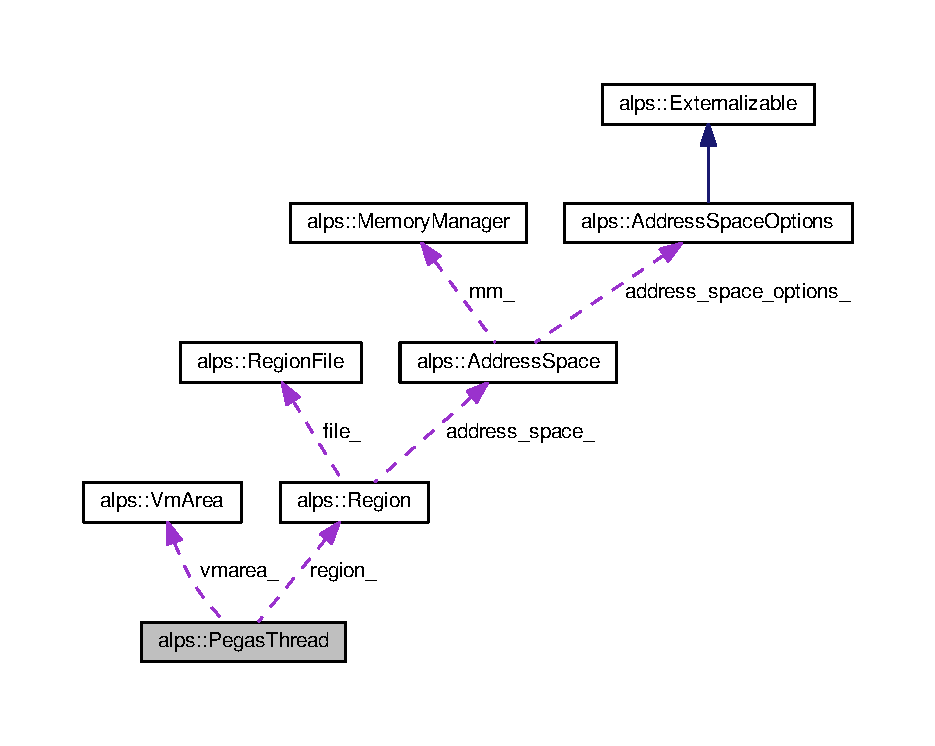
\includegraphics[width=350pt]{classalps_1_1PegasThread__coll__graph}
\end{center}
\end{figure}
\subsection*{Public Member Functions}
\begin{DoxyCompactItemize}
\item 
void {\bfseries set\+\_\+active\+\_\+pregion} (\hyperlink{classalps_1_1Region}{Region} $\ast$region)\hypertarget{classalps_1_1PegasThread_a9dda39658cc11f48d4eb4d7e8528866a}{}\label{classalps_1_1PegasThread_a9dda39658cc11f48d4eb4d7e8528866a}

\end{DoxyCompactItemize}
\subsection*{Public Attributes}
\begin{DoxyCompactItemize}
\item 
\hyperlink{classalps_1_1Region}{Region} $\ast$ {\bfseries region\+\_\+}\hypertarget{classalps_1_1PegasThread_aa6495df538b6beb29f6515321572b07f}{}\label{classalps_1_1PegasThread_aa6495df538b6beb29f6515321572b07f}

\item 
uint64\+\_\+t {\bfseries vmarea\+\_\+version\+\_\+}\hypertarget{classalps_1_1PegasThread_a01a36ffdbda7b3e97fdf801bfa618052}{}\label{classalps_1_1PegasThread_a01a36ffdbda7b3e97fdf801bfa618052}

\item 
\hyperlink{classalps_1_1VmArea}{Vm\+Area} $\ast$ {\bfseries vmarea\+\_\+}\hypertarget{classalps_1_1PegasThread_a0d3aca0aaafe8c9094ee5175ec23467d}{}\label{classalps_1_1PegasThread_a0d3aca0aaafe8c9094ee5175ec23467d}

\end{DoxyCompactItemize}


The documentation for this class was generated from the following file\+:\begin{DoxyCompactItemize}
\item 
/home/yuan/\+Benchmarks/whisper/mnemosyne-\/gcc/usermode/library/pmalloc/include/alps/src/pegasus/pegasthread.\+hh\end{DoxyCompactItemize}

\hypertarget{classalps_1_1Pegasus}{}\section{alps\+:\+:Pegasus Class Reference}
\label{classalps_1_1Pegasus}\index{alps\+::\+Pegasus@{alps\+::\+Pegasus}}


\hyperlink{classalps_1_1Pegasus}{Pegasus} environment.  




{\ttfamily \#include $<$pegasus.\+hh$>$}



Collaboration diagram for alps\+:\+:Pegasus\+:
\nopagebreak
\begin{figure}[H]
\begin{center}
\leavevmode
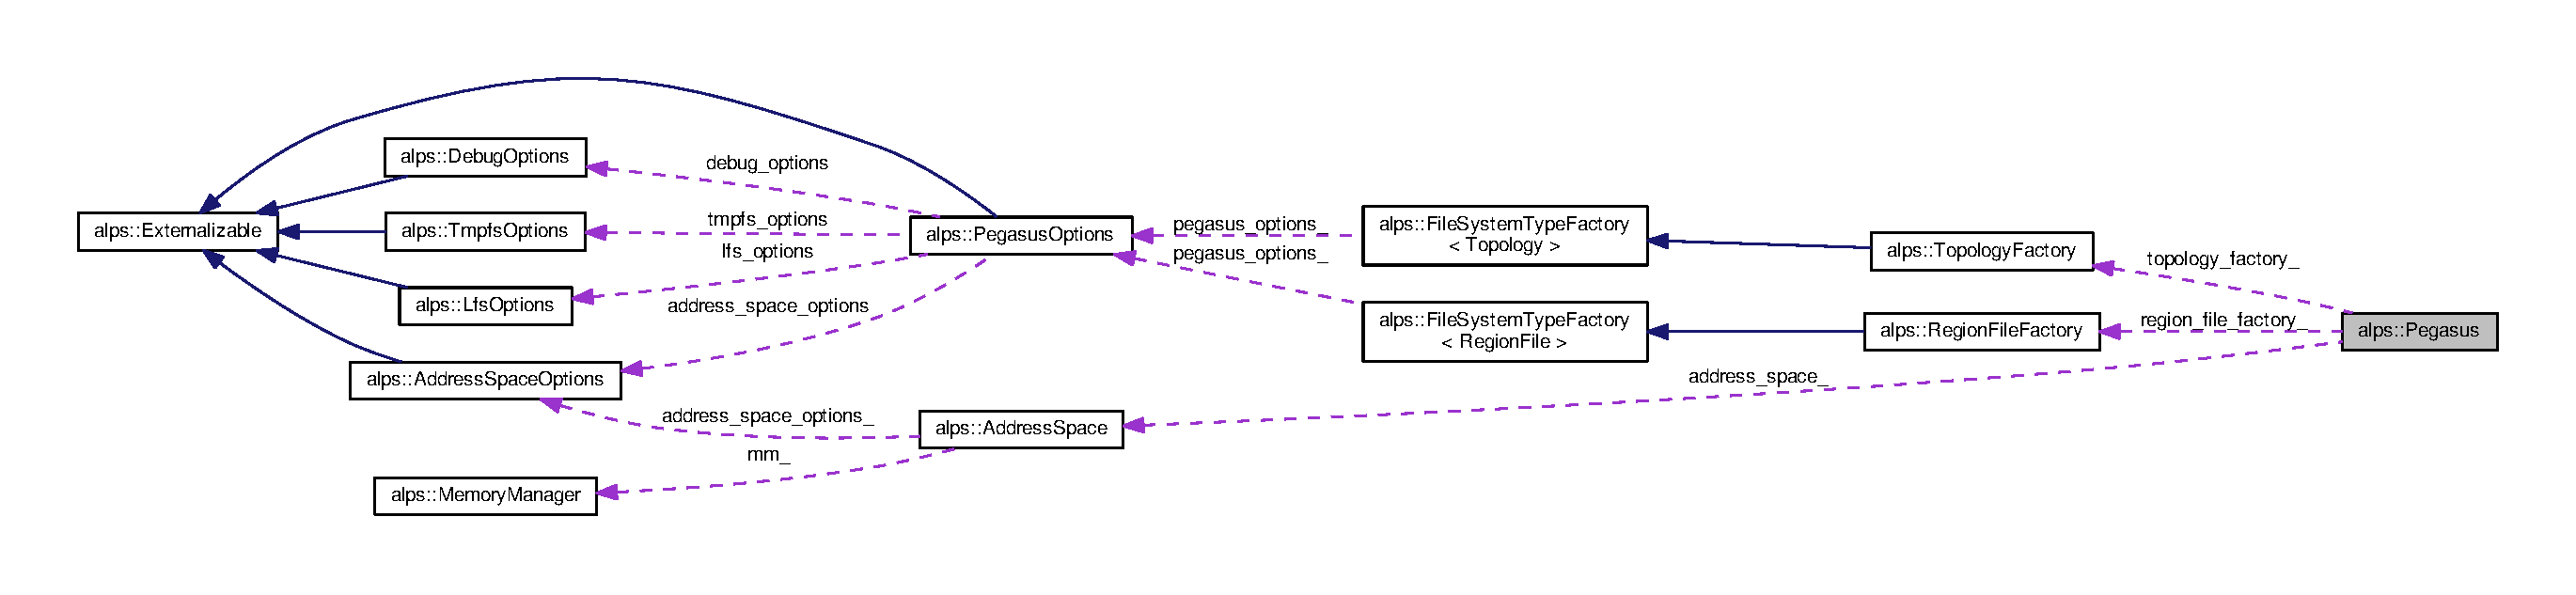
\includegraphics[width=350pt]{classalps_1_1Pegasus__coll__graph}
\end{center}
\end{figure}
\subsection*{Static Public Member Functions}
\begin{DoxyCompactItemize}
\item 
static \hyperlink{classalps_1_1ErrorStack}{Error\+Stack} \hyperlink{classalps_1_1Pegasus_acc5a6c8a6a29fb20c52088fa01602c94}{load\+\_\+options} (const char $\ast$config\+\_\+file, bool use\+\_\+system\+\_\+wide\+\_\+conf, bool use\+\_\+environ, \hyperlink{structalps_1_1PegasusOptions}{Pegasus\+Options} $\ast$pegasus\+\_\+options)
\begin{DoxyCompactList}\small\item\em Loads configuration options from configuration file into object pointed by {\itshape pegasus\+\_\+options}. \end{DoxyCompactList}\item 
static \hyperlink{classalps_1_1ErrorStack}{Error\+Stack} \hyperlink{classalps_1_1Pegasus_a69e9d95ce8c4d350871dea4929fcf53b}{init} (const char $\ast$config\+\_\+file, bool use\+\_\+system\+\_\+wide\+\_\+conf, bool use\+\_\+environ)
\begin{DoxyCompactList}\small\item\em Initialize \hyperlink{classalps_1_1Pegasus}{Pegasus} singleton class by loading configuration options from a file. \end{DoxyCompactList}\item 
static \hyperlink{classalps_1_1ErrorStack}{Error\+Stack} \hyperlink{classalps_1_1Pegasus_a7dd3ac592651ab750897104e6006d310}{init} (const \hyperlink{structalps_1_1PegasusOptions}{Pegasus\+Options} \&pegasus\+\_\+options)\hypertarget{classalps_1_1Pegasus_a7dd3ac592651ab750897104e6006d310}{}\label{classalps_1_1Pegasus_a7dd3ac592651ab750897104e6006d310}

\begin{DoxyCompactList}\small\item\em Initialize \hyperlink{classalps_1_1Pegasus}{Pegasus} singleton class by loading configuration options from options object {\itshape pegasus\+\_\+options}. \end{DoxyCompactList}\item 
static \hyperlink{group__ERRORCODES_ga6263a3c9a0b8d36aea21cdd835ac99fe}{Error\+Code} {\bfseries create\+\_\+region\+\_\+file} (const char $\ast$pathname, mode\+\_\+t mode, \hyperlink{classalps_1_1RegionFile}{Region\+File} $\ast$$\ast$region\+\_\+file)\hypertarget{classalps_1_1Pegasus_a5dedaa1c31fa7bd9be92e9773b1f5a0a}{}\label{classalps_1_1Pegasus_a5dedaa1c31fa7bd9be92e9773b1f5a0a}

\item 
static \hyperlink{group__ERRORCODES_ga6263a3c9a0b8d36aea21cdd835ac99fe}{Error\+Code} {\bfseries open\+\_\+region\+\_\+file} (const char $\ast$pathname, int flags, mode\+\_\+t mode, \hyperlink{classalps_1_1RegionFile}{Region\+File} $\ast$$\ast$region\+\_\+file)\hypertarget{classalps_1_1Pegasus_aa7330693d15beebbf829e296a984a5a7}{}\label{classalps_1_1Pegasus_aa7330693d15beebbf829e296a984a5a7}

\item 
static \hyperlink{group__ERRORCODES_ga6263a3c9a0b8d36aea21cdd835ac99fe}{Error\+Code} {\bfseries open\+\_\+region\+\_\+file} (const char $\ast$$\ast$pathnames, int npathnames, int flags, mode\+\_\+t mode, \hyperlink{classalps_1_1RegionFile}{Region\+File} $\ast$$\ast$region\+\_\+file)\hypertarget{classalps_1_1Pegasus_a1674c4a5dbb6b199f629294b7693b8db}{}\label{classalps_1_1Pegasus_a1674c4a5dbb6b199f629294b7693b8db}

\item 
static \hyperlink{group__ERRORCODES_ga6263a3c9a0b8d36aea21cdd835ac99fe}{Error\+Code} {\bfseries open\+\_\+region\+\_\+file} (const char $\ast$pathname, int flags, \hyperlink{classalps_1_1RegionFile}{Region\+File} $\ast$$\ast$region\+\_\+file)\hypertarget{classalps_1_1Pegasus_aa9131da83f3334082f097d6cf4126646}{}\label{classalps_1_1Pegasus_aa9131da83f3334082f097d6cf4126646}

\item 
static \hyperlink{group__ERRORCODES_ga6263a3c9a0b8d36aea21cdd835ac99fe}{Error\+Code} {\bfseries open\+\_\+region\+\_\+file} (const char $\ast$$\ast$pathnames, int npathnames, int flags, \hyperlink{classalps_1_1RegionFile}{Region\+File} $\ast$$\ast$region\+\_\+file)\hypertarget{classalps_1_1Pegasus_af7e9d5041fe8dd956fb1c16df120ec4e}{}\label{classalps_1_1Pegasus_af7e9d5041fe8dd956fb1c16df120ec4e}

\item 
static \hyperlink{classalps_1_1AddressSpace}{Address\+Space} $\ast$ {\bfseries address\+\_\+space} ()\hypertarget{classalps_1_1Pegasus_a0994d567bc6c509972d3f92223482445}{}\label{classalps_1_1Pegasus_a0994d567bc6c509972d3f92223482445}

\item 
static \hyperlink{classalps_1_1RegionFileFactory}{Region\+File\+Factory} $\ast$ {\bfseries region\+\_\+file\+\_\+factory} ()\hypertarget{classalps_1_1Pegasus_a5d35cbc08b21204f62dd47d901a81d44}{}\label{classalps_1_1Pegasus_a5d35cbc08b21204f62dd47d901a81d44}

\item 
static \hyperlink{classalps_1_1TopologyFactory}{Topology\+Factory} $\ast$ {\bfseries topology\+\_\+factory} ()\hypertarget{classalps_1_1Pegasus_a6959ebba3ef27f5baad94a2aaa25bd52}{}\label{classalps_1_1Pegasus_a6959ebba3ef27f5baad94a2aaa25bd52}

\end{DoxyCompactItemize}
\subsection*{Static Protected Attributes}
\begin{DoxyCompactItemize}
\item 
static \hyperlink{classalps_1_1AddressSpace}{Address\+Space} $\ast$ {\bfseries address\+\_\+space\+\_\+}\hypertarget{classalps_1_1Pegasus_aa36d35213146588133d73f4de0e049ad}{}\label{classalps_1_1Pegasus_aa36d35213146588133d73f4de0e049ad}

\item 
static \hyperlink{classalps_1_1RegionFileFactory}{Region\+File\+Factory} $\ast$ {\bfseries region\+\_\+file\+\_\+factory\+\_\+}\hypertarget{classalps_1_1Pegasus_a9adc08b25e2a59f03bf77fc52bfac30a}{}\label{classalps_1_1Pegasus_a9adc08b25e2a59f03bf77fc52bfac30a}

\item 
static \hyperlink{classalps_1_1TopologyFactory}{Topology\+Factory} $\ast$ {\bfseries topology\+\_\+factory\+\_\+}\hypertarget{classalps_1_1Pegasus_a5c73a1692f85dbfb278ba21f80dab228}{}\label{classalps_1_1Pegasus_a5c73a1692f85dbfb278ba21f80dab228}

\end{DoxyCompactItemize}


\subsection{Detailed Description}
A static singleton class that encapsulates a \hyperlink{classalps_1_1Pegasus}{Pegasus} environment 

\subsection{Member Function Documentation}
\index{alps\+::\+Pegasus@{alps\+::\+Pegasus}!init@{init}}
\index{init@{init}!alps\+::\+Pegasus@{alps\+::\+Pegasus}}
\subsubsection[{\texorpdfstring{init(const char $\ast$config\+\_\+file, bool use\+\_\+system\+\_\+wide\+\_\+conf, bool use\+\_\+environ)}{init(const char *config_file, bool use_system_wide_conf, bool use_environ)}}]{\setlength{\rightskip}{0pt plus 5cm}{\bf Error\+Stack} alps\+::\+Pegasus\+::init (
\begin{DoxyParamCaption}
\item[{const char $\ast$}]{config\+\_\+file, }
\item[{bool}]{use\+\_\+system\+\_\+wide\+\_\+conf, }
\item[{bool}]{use\+\_\+environ}
\end{DoxyParamCaption}
)\hspace{0.3cm}{\ttfamily [static]}}\hypertarget{classalps_1_1Pegasus_a69e9d95ce8c4d350871dea4929fcf53b}{}\label{classalps_1_1Pegasus_a69e9d95ce8c4d350871dea4929fcf53b}
A shorthand for \hyperlink{classalps_1_1Pegasus_acc5a6c8a6a29fb20c52088fa01602c94}{load\+\_\+options()} followed by init(\+Pegasus\+Options$\ast$).

Load configurations options in the order described under load\+\_\+options. \index{alps\+::\+Pegasus@{alps\+::\+Pegasus}!load\+\_\+options@{load\+\_\+options}}
\index{load\+\_\+options@{load\+\_\+options}!alps\+::\+Pegasus@{alps\+::\+Pegasus}}
\subsubsection[{\texorpdfstring{load\+\_\+options(const char $\ast$config\+\_\+file, bool use\+\_\+system\+\_\+wide\+\_\+conf, bool use\+\_\+environ, Pegasus\+Options $\ast$pegasus\+\_\+options)}{load_options(const char *config_file, bool use_system_wide_conf, bool use_environ, PegasusOptions *pegasus_options)}}]{\setlength{\rightskip}{0pt plus 5cm}{\bf Error\+Stack} alps\+::\+Pegasus\+::load\+\_\+options (
\begin{DoxyParamCaption}
\item[{const char $\ast$}]{config\+\_\+file, }
\item[{bool}]{use\+\_\+system\+\_\+wide\+\_\+conf, }
\item[{bool}]{use\+\_\+environ, }
\item[{{\bf Pegasus\+Options} $\ast$}]{pegasus\+\_\+options}
\end{DoxyParamCaption}
)\hspace{0.3cm}{\ttfamily [static]}}\hypertarget{classalps_1_1Pegasus_acc5a6c8a6a29fb20c52088fa01602c94}{}\label{classalps_1_1Pegasus_acc5a6c8a6a29fb20c52088fa01602c94}
Caller is responsible to pass a valid \hyperlink{structalps_1_1PegasusOptions}{Pegasus\+Options} object

Load configuration options in the following order\+:
\begin{DoxyItemize}
\item If {\itshape use\+\_\+system\+\_\+wide\+\_\+conf} is then load configuration options from the system wide configuration file (/etc/default/alps.yml), and then
\item If path {\itshape use\+\_\+environ} is set then load configuration options from the file declared by environment variable A\+L\+P\+S\+\_\+\+C\+O\+NF, and then
\item Load configuration options from {\itshape config\+\_\+file}. 
\end{DoxyItemize}

The documentation for this class was generated from the following files\+:\begin{DoxyCompactItemize}
\item 
/home/yuan/\+Benchmarks/whisper/mnemosyne-\/gcc/usermode/library/pmalloc/include/alps/include/alps/pegasus/pegasus.\+hh\item 
/home/yuan/\+Benchmarks/whisper/mnemosyne-\/gcc/usermode/library/pmalloc/include/alps/src/pegasus/pegasus.\+cc\end{DoxyCompactItemize}

\hypertarget{structalps_1_1PegasusOptions}{}\section{alps\+:\+:Pegasus\+Options Struct Reference}
\label{structalps_1_1PegasusOptions}\index{alps\+::\+Pegasus\+Options@{alps\+::\+Pegasus\+Options}}


Inheritance diagram for alps\+:\+:Pegasus\+Options\+:
\nopagebreak
\begin{figure}[H]
\begin{center}
\leavevmode
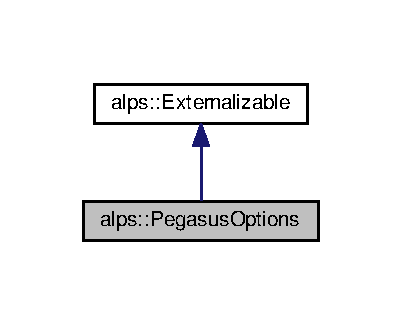
\includegraphics[width=193pt]{structalps_1_1PegasusOptions__inherit__graph}
\end{center}
\end{figure}


Collaboration diagram for alps\+:\+:Pegasus\+Options\+:
\nopagebreak
\begin{figure}[H]
\begin{center}
\leavevmode
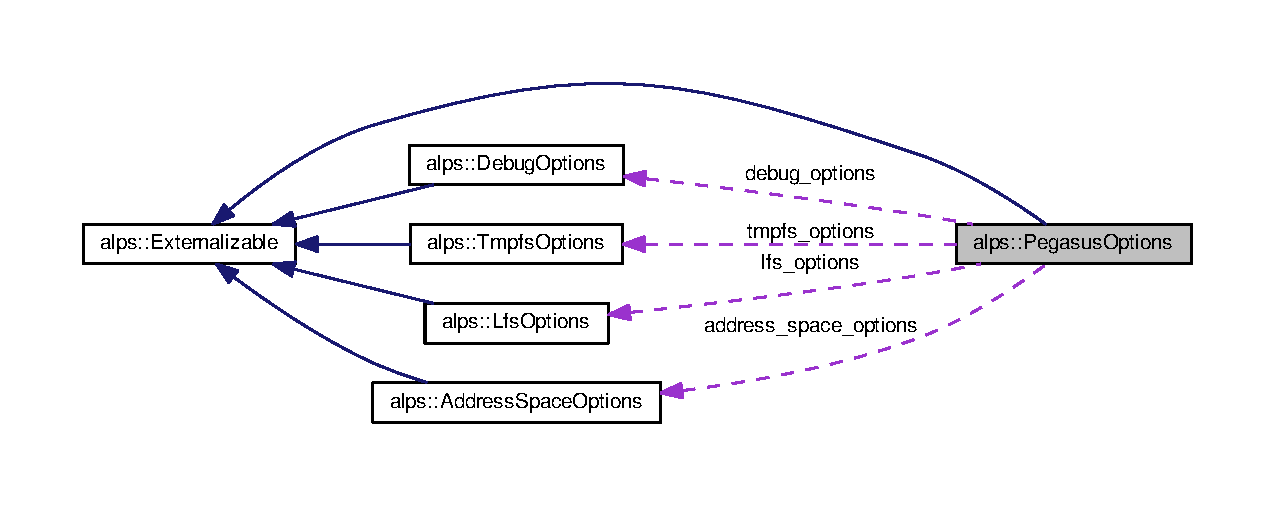
\includegraphics[width=350pt]{structalps_1_1PegasusOptions__coll__graph}
\end{center}
\end{figure}
\subsection*{Public Member Functions}
\begin{DoxyCompactItemize}
\item 
{\bfseries E\+X\+T\+E\+R\+N\+A\+L\+I\+Z\+A\+B\+LE} (\hyperlink{structalps_1_1PegasusOptions}{Pegasus\+Options})\hypertarget{structalps_1_1PegasusOptions_afdff20a8d8b89d05a7d2d9126e852638}{}\label{structalps_1_1PegasusOptions_afdff20a8d8b89d05a7d2d9126e852638}

\end{DoxyCompactItemize}
\subsection*{Public Attributes}
\begin{DoxyCompactItemize}
\item 
\hyperlink{structalps_1_1AddressSpaceOptions}{Address\+Space\+Options} {\bfseries address\+\_\+space\+\_\+options}\hypertarget{structalps_1_1PegasusOptions_a24e2c4559ffde41961bfdbbfeeb756a0}{}\label{structalps_1_1PegasusOptions_a24e2c4559ffde41961bfdbbfeeb756a0}

\item 
\hyperlink{structalps_1_1DebugOptions}{Debug\+Options} {\bfseries debug\+\_\+options}\hypertarget{structalps_1_1PegasusOptions_ae71cf8e8ba799b2004c99568667f68e4}{}\label{structalps_1_1PegasusOptions_ae71cf8e8ba799b2004c99568667f68e4}

\item 
\hyperlink{structalps_1_1LfsOptions}{Lfs\+Options} {\bfseries lfs\+\_\+options}\hypertarget{structalps_1_1PegasusOptions_a46d4088a2b1f4a4f010ad42c0dfd80d1}{}\label{structalps_1_1PegasusOptions_a46d4088a2b1f4a4f010ad42c0dfd80d1}

\item 
\hyperlink{structalps_1_1TmpfsOptions}{Tmpfs\+Options} {\bfseries tmpfs\+\_\+options}\hypertarget{structalps_1_1PegasusOptions_ad924df0f443185396961db63d76e20c3}{}\label{structalps_1_1PegasusOptions_ad924df0f443185396961db63d76e20c3}

\end{DoxyCompactItemize}
\subsection*{Additional Inherited Members}


The documentation for this struct was generated from the following file\+:\begin{DoxyCompactItemize}
\item 
/home/yuan/\+Benchmarks/whisper/mnemosyne-\/gcc/usermode/library/pmalloc/include/alps/include/alps/pegasus/pegasus\+\_\+options.\+hh\end{DoxyCompactItemize}

\hypertarget{classalps_1_1BaseRelativePointer_1_1PPtr}{}\section{alps\+:\+:Base\+Relative\+Pointer\+:\+:P\+Ptr$<$ Region\+Type, Pointed\+Type $>$ Class Template Reference}
\label{classalps_1_1BaseRelativePointer_1_1PPtr}\index{alps\+::\+Base\+Relative\+Pointer\+::\+P\+Ptr$<$ Region\+Type, Pointed\+Type $>$@{alps\+::\+Base\+Relative\+Pointer\+::\+P\+Ptr$<$ Region\+Type, Pointed\+Type $>$}}


Represents a linear persistent pointer.  




{\ttfamily \#include $<$pointer.\+hh$>$}



Collaboration diagram for alps\+:\+:Base\+Relative\+Pointer\+:\+:P\+Ptr$<$ Region\+Type, Pointed\+Type $>$\+:
\nopagebreak
\begin{figure}[H]
\begin{center}
\leavevmode
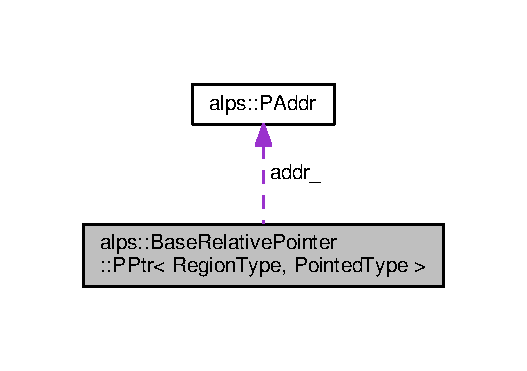
\includegraphics[width=253pt]{classalps_1_1BaseRelativePointer_1_1PPtr__coll__graph}
\end{center}
\end{figure}
\subsection*{Public Types}
\begin{DoxyCompactItemize}
\item 
typedef Pointed\+Type $\ast$ {\bfseries pointer}\hypertarget{classalps_1_1BaseRelativePointer_1_1PPtr_a5f717b3a58c7c552bf047eea9f22fb6c}{}\label{classalps_1_1BaseRelativePointer_1_1PPtr_a5f717b3a58c7c552bf047eea9f22fb6c}

\item 
typedef boost\+::add\+\_\+reference$<$ Pointed\+Type $>$\+::type {\bfseries reference}\hypertarget{classalps_1_1BaseRelativePointer_1_1PPtr_a88f51b3310a8e4422bf1391f1a88d8d9}{}\label{classalps_1_1BaseRelativePointer_1_1PPtr_a88f51b3310a8e4422bf1391f1a88d8d9}

\end{DoxyCompactItemize}
\subsection*{Public Member Functions}
\begin{DoxyCompactItemize}
\item 
{\bfseries P\+Ptr} (Linear\+Addr offset)\hypertarget{classalps_1_1BaseRelativePointer_1_1PPtr_a3d30f50e8ff9606e1a70e9243e7435c5}{}\label{classalps_1_1BaseRelativePointer_1_1PPtr_a3d30f50e8ff9606e1a70e9243e7435c5}

\item 
{\bfseries P\+Ptr} (const \hyperlink{classalps_1_1BaseRelativePointer_1_1PPtr}{P\+Ptr}$<$ Region\+Type, void $>$ \&other)\hypertarget{classalps_1_1BaseRelativePointer_1_1PPtr_a72d3074d889b18799a26545ff70fb9fc}{}\label{classalps_1_1BaseRelativePointer_1_1PPtr_a72d3074d889b18799a26545ff70fb9fc}

\item 
{\bfseries P\+Ptr} (\hyperlink{classalps_1_1BaseRelativePointer_1_1IPtr}{I\+Ptr}$<$ Region\+Type, Pointed\+Type $>$ \&other)\hypertarget{classalps_1_1BaseRelativePointer_1_1PPtr_af2c23a1a1e4a25b955c0a19e742734f1}{}\label{classalps_1_1BaseRelativePointer_1_1PPtr_af2c23a1a1e4a25b955c0a19e742734f1}

\item 
{\bfseries operator I\+Ptr$<$ Region\+Type, Pointed\+Type $>$} ()\hypertarget{classalps_1_1BaseRelativePointer_1_1PPtr_acea6bf55fc7565381b9dde632f0d8efc}{}\label{classalps_1_1BaseRelativePointer_1_1PPtr_acea6bf55fc7565381b9dde632f0d8efc}

\item 
\hyperlink{classalps_1_1BaseRelativePointer_1_1PPtr}{P\+Ptr} \& {\bfseries operator=} (Pointed\+Type $\ast$from)\hypertarget{classalps_1_1BaseRelativePointer_1_1PPtr_aafa170c5c498ad4f508f88fc0ae6ec38}{}\label{classalps_1_1BaseRelativePointer_1_1PPtr_aafa170c5c498ad4f508f88fc0ae6ec38}

\item 
\hyperlink{classalps_1_1BaseRelativePointer_1_1PPtr}{P\+Ptr} \& {\bfseries operator=} (const \hyperlink{classalps_1_1BaseRelativePointer_1_1IPtr}{I\+Ptr}$<$ Region\+Type, Pointed\+Type $>$ \&other)\hypertarget{classalps_1_1BaseRelativePointer_1_1PPtr_a788caa799b260204b7d39fe6de99fd0f}{}\label{classalps_1_1BaseRelativePointer_1_1PPtr_a788caa799b260204b7d39fe6de99fd0f}

\item 
\hyperlink{classalps_1_1BaseRelativePointer_1_1PPtr}{P\+Ptr} \& {\bfseries operator=} (const \hyperlink{classalps_1_1BaseRelativePointer_1_1TPtr}{T\+Ptr}$<$ Region\+Type, Pointed\+Type $>$ \&tptr)\hypertarget{classalps_1_1BaseRelativePointer_1_1PPtr_ad802b446e818406ec4295efade695a1e}{}\label{classalps_1_1BaseRelativePointer_1_1PPtr_ad802b446e818406ec4295efade695a1e}

\item 
pointer {\bfseries get} () const \hypertarget{classalps_1_1BaseRelativePointer_1_1PPtr_a4a0ca4093873f2dab30e990cd8174dd7}{}\label{classalps_1_1BaseRelativePointer_1_1PPtr_a4a0ca4093873f2dab30e990cd8174dd7}

\item 
pointer {\bfseries operator-\/$>$} () const \hypertarget{classalps_1_1BaseRelativePointer_1_1PPtr_ac823159a9ea8a2f901ff061c59664565}{}\label{classalps_1_1BaseRelativePointer_1_1PPtr_ac823159a9ea8a2f901ff061c59664565}

\item 
reference {\bfseries operator$\ast$} () const \hypertarget{classalps_1_1BaseRelativePointer_1_1PPtr_a4cd8e0384027d714e3ceb5c217db38ad}{}\label{classalps_1_1BaseRelativePointer_1_1PPtr_a4cd8e0384027d714e3ceb5c217db38ad}

\item 
bool {\bfseries operator==} (const \hyperlink{classalps_1_1BaseRelativePointer_1_1IPtr}{I\+Ptr}$<$ Region\+Type, Pointed\+Type $>$ \&other\+\_\+iptr) const \hypertarget{classalps_1_1BaseRelativePointer_1_1PPtr_adbaccb816260a3431aaa33c12397e0c6}{}\label{classalps_1_1BaseRelativePointer_1_1PPtr_adbaccb816260a3431aaa33c12397e0c6}

\item 
bool {\bfseries operator!=} (const \hyperlink{classalps_1_1BaseRelativePointer_1_1IPtr}{I\+Ptr}$<$ Region\+Type, Pointed\+Type $>$ \&other\+\_\+iptr) const \hypertarget{classalps_1_1BaseRelativePointer_1_1PPtr_a20a5a643be92c5cd98ad2b3496831c33}{}\label{classalps_1_1BaseRelativePointer_1_1PPtr_a20a5a643be92c5cd98ad2b3496831c33}

\item 
reference {\bfseries operator\mbox{[}$\,$\mbox{]}} (std\+::ptrdiff\+\_\+t idx) const \hypertarget{classalps_1_1BaseRelativePointer_1_1PPtr_a7e32a2e734ef7725c125f24f73d82ce7}{}\label{classalps_1_1BaseRelativePointer_1_1PPtr_a7e32a2e734ef7725c125f24f73d82ce7}

\item 
\hyperlink{classalps_1_1BaseRelativePointer_1_1TPtr}{T\+Ptr}$<$ Region\+Type, Pointed\+Type $>$ {\bfseries operator+} (std\+::ptrdiff\+\_\+t offset) const \hypertarget{classalps_1_1BaseRelativePointer_1_1PPtr_a859680f5e1d4838dd30d09e8c17f3a71}{}\label{classalps_1_1BaseRelativePointer_1_1PPtr_a859680f5e1d4838dd30d09e8c17f3a71}

\item 
void {\bfseries stream\+\_\+to} (std\+::ostream \&os) const \hypertarget{classalps_1_1BaseRelativePointer_1_1PPtr_ac840656da125bdf6d480a5794e7d13ee}{}\label{classalps_1_1BaseRelativePointer_1_1PPtr_ac840656da125bdf6d480a5794e7d13ee}

\end{DoxyCompactItemize}
\subsection*{Public Attributes}
\begin{DoxyCompactItemize}
\item 
\hyperlink{structalps_1_1PAddr}{P\+Addr} {\bfseries addr\+\_\+}\hypertarget{classalps_1_1BaseRelativePointer_1_1PPtr_a90eca717658a9ca6943ae4172393a759}{}\label{classalps_1_1BaseRelativePointer_1_1PPtr_a90eca717658a9ca6943ae4172393a759}

\end{DoxyCompactItemize}


\subsection{Detailed Description}
\subsubsection*{template$<$typename Region\+Type, typename Pointed\+Type$>$\\*
class alps\+::\+Base\+Relative\+Pointer\+::\+P\+Ptr$<$ Region\+Type, Pointed\+Type $>$}

Represents a smart persistent pointer that points to a persistent logical linear address (i.\+e., the pointer stores a persistent logical linear address). The pointer is valid for exchanging and sharing a reference to memory location among multiple processes mapping a region. It works with both fixed virtual address mappings and relocatable regions. It does not support inter-\/region pointers. 

The documentation for this class was generated from the following file\+:\begin{DoxyCompactItemize}
\item 
/home/yuan/\+Benchmarks/whisper/mnemosyne-\/gcc/usermode/library/pmalloc/include/alps/include/alps/pegasus/pointer.\+hh\end{DoxyCompactItemize}

\hypertarget{classalps_1_1ProcessMap}{}\section{alps\+:\+:Process\+Map Class Reference}
\label{classalps_1_1ProcessMap}\index{alps\+::\+Process\+Map@{alps\+::\+Process\+Map}}
\subsection*{Public Member Functions}
\begin{DoxyCompactItemize}
\item 
{\bfseries Process\+Map} (pid\+\_\+t pid)\hypertarget{classalps_1_1ProcessMap_af5fb1aac3fccdfe185ab9eaaca4deb23}{}\label{classalps_1_1ProcessMap_af5fb1aac3fccdfe185ab9eaaca4deb23}

\item 
std\+::pair$<$ size\+\_\+t, size\+\_\+t $>$ {\bfseries range} (const std\+::string name)\hypertarget{classalps_1_1ProcessMap_a788dce0ccbd6e9270492230f04cad506}{}\label{classalps_1_1ProcessMap_a788dce0ccbd6e9270492230f04cad506}

\end{DoxyCompactItemize}


The documentation for this class was generated from the following files\+:\begin{DoxyCompactItemize}
\item 
/home/yuan/\+Benchmarks/whisper/mnemosyne-\/gcc/usermode/library/pmalloc/include/alps/src/common/os.\+hh\item 
/home/yuan/\+Benchmarks/whisper/mnemosyne-\/gcc/usermode/library/pmalloc/include/alps/src/common/os.\+cc\end{DoxyCompactItemize}

\hypertarget{classalps_1_1Region}{}\section{alps\+:\+:Region Class Reference}
\label{classalps_1_1Region}\index{alps\+::\+Region@{alps\+::\+Region}}


Persistent memory region.  




{\ttfamily \#include $<$region.\+hh$>$}



Collaboration diagram for alps\+:\+:Region\+:
\nopagebreak
\begin{figure}[H]
\begin{center}
\leavevmode
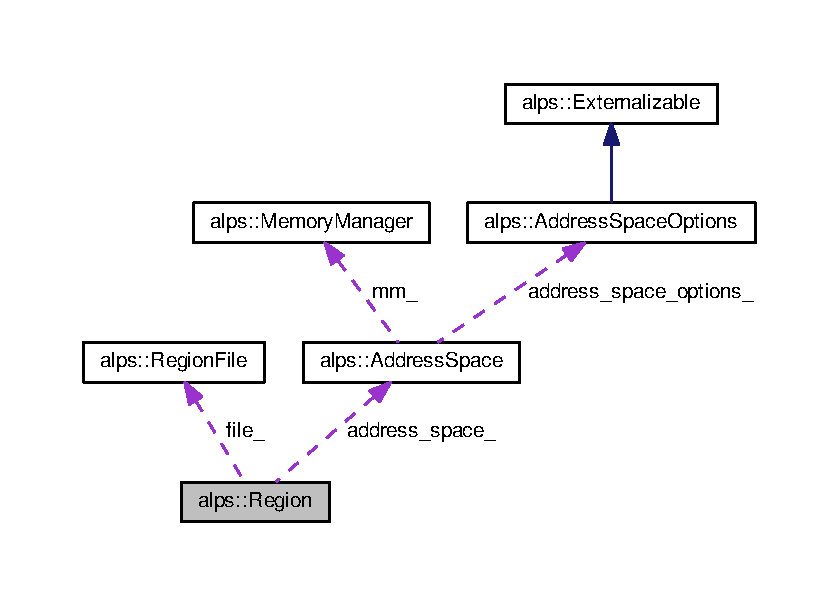
\includegraphics[width=350pt]{classalps_1_1Region__coll__graph}
\end{center}
\end{figure}
\subsection*{Public Member Functions}
\begin{DoxyCompactItemize}
\item 
{\bfseries Region} (\hyperlink{classalps_1_1AddressSpace}{Address\+Space} $\ast$\hyperlink{classalps_1_1Region_a0468534d0b84744f4ae689afb13ae0b5}{address\+\_\+space}, \hyperlink{classalps_1_1RegionFile}{Region\+File} $\ast$region\+\_\+file)\hypertarget{classalps_1_1Region_a49be6b716e4cd1ac246c51c975511438}{}\label{classalps_1_1Region_a49be6b716e4cd1ac246c51c975511438}

\item 
\hyperlink{classalps_1_1RegionFile}{Region\+File} $\ast$ \hyperlink{classalps_1_1Region_ace503ff06288ae02cae4f9b2b7b391d8}{file} ()\hypertarget{classalps_1_1Region_ace503ff06288ae02cae4f9b2b7b391d8}{}\label{classalps_1_1Region_ace503ff06288ae02cae4f9b2b7b391d8}

\begin{DoxyCompactList}\small\item\em Returns the region file backing this region. \end{DoxyCompactList}\item 
loff\+\_\+t {\bfseries length} ()\hypertarget{classalps_1_1Region_affad93da622e09a41e9c5a78cf724fac}{}\label{classalps_1_1Region_affad93da622e09a41e9c5a78cf724fac}

\item 
Region\+Id \hyperlink{classalps_1_1Region_a44af36c129f944a859a1ef45bd1ddf74}{id} ()\hypertarget{classalps_1_1Region_a44af36c129f944a859a1ef45bd1ddf74}{}\label{classalps_1_1Region_a44af36c129f944a859a1ef45bd1ddf74}

\begin{DoxyCompactList}\small\item\em Returns a global identifier identifying the region. \end{DoxyCompactList}\item 
\hyperlink{classalps_1_1AddressSpace}{Address\+Space} $\ast$ \hyperlink{classalps_1_1Region_a0468534d0b84744f4ae689afb13ae0b5}{address\+\_\+space} ()\hypertarget{classalps_1_1Region_a0468534d0b84744f4ae689afb13ae0b5}{}\label{classalps_1_1Region_a0468534d0b84744f4ae689afb13ae0b5}

\begin{DoxyCompactList}\small\item\em Returns the Address Space object the region is mapped to. \end{DoxyCompactList}\item 
\hyperlink{group__ERRORCODES_ga6263a3c9a0b8d36aea21cdd835ac99fe}{Error\+Code} \hyperlink{classalps_1_1Region_a61ad82fe33c08b158c0ec5dec9403f8c}{set\+\_\+interleave\+\_\+group} (loff\+\_\+t offset, loff\+\_\+t length, const std\+::vector$<$ Interleave\+Group $>$ \&vig)\hypertarget{classalps_1_1Region_a61ad82fe33c08b158c0ec5dec9403f8c}{}\label{classalps_1_1Region_a61ad82fe33c08b158c0ec5dec9403f8c}

\begin{DoxyCompactList}\small\item\em Sets interleave group hint for pages mapped in the range \mbox{[}{\itshape offset}, {\itshape offset} + {\itshape length}). \end{DoxyCompactList}\item 
\hyperlink{group__ERRORCODES_ga6263a3c9a0b8d36aea21cdd835ac99fe}{Error\+Code} \hyperlink{classalps_1_1Region_adf07690fef596f4839404b3651019640}{interleave\+\_\+group} (loff\+\_\+t offset, loff\+\_\+t length, std\+::vector$<$ Interleave\+Group $>$ $\ast$vig)\hypertarget{classalps_1_1Region_adf07690fef596f4839404b3651019640}{}\label{classalps_1_1Region_adf07690fef596f4839404b3651019640}

\begin{DoxyCompactList}\small\item\em Returns assigned interleave group for pages mapped in the range \mbox{[}{\itshape offset}, {\itshape offset} + {\itshape length}). \end{DoxyCompactList}\end{DoxyCompactItemize}
\subsection*{Protected Attributes}
\begin{DoxyCompactItemize}
\item 
Region\+Id {\bfseries region\+\_\+id\+\_\+}\hypertarget{classalps_1_1Region_a0742daaa798c7f500c3cf6ec624a2a1c}{}\label{classalps_1_1Region_a0742daaa798c7f500c3cf6ec624a2a1c}

\item 
\hyperlink{classalps_1_1AddressSpace}{Address\+Space} $\ast$ {\bfseries address\+\_\+space\+\_\+}\hypertarget{classalps_1_1Region_a58a86cf05f9f3f6de58fb05be7a5e0ec}{}\label{classalps_1_1Region_a58a86cf05f9f3f6de58fb05be7a5e0ec}

\item 
loff\+\_\+t \hyperlink{classalps_1_1Region_ac55de996c3c976303cfe396034565f12}{length\+\_\+}\hypertarget{classalps_1_1Region_ac55de996c3c976303cfe396034565f12}{}\label{classalps_1_1Region_ac55de996c3c976303cfe396034565f12}

\begin{DoxyCompactList}\small\item\em cached value of the backing file\textquotesingle{}s length \end{DoxyCompactList}\item 
\hyperlink{classalps_1_1RegionFile}{Region\+File} $\ast$ \hyperlink{classalps_1_1Region_a4212a00156815c7d00b221086e9d30f3}{file\+\_\+}\hypertarget{classalps_1_1Region_a4212a00156815c7d00b221086e9d30f3}{}\label{classalps_1_1Region_a4212a00156815c7d00b221086e9d30f3}

\begin{DoxyCompactList}\small\item\em the file backing the persistent memory region \end{DoxyCompactList}\end{DoxyCompactItemize}


\subsection{Detailed Description}
A base class that represents a persistent memory region in the logical address space (\hyperlink{classalps_1_1AddressSpace}{alps\+::\+Address\+Space}).

A region is instantiated by mapping (and optionally binding) a region file (or a set of region files) to an \hyperlink{classalps_1_1AddressSpace}{Address\+Space} object. 

The documentation for this class was generated from the following files\+:\begin{DoxyCompactItemize}
\item 
/home/yuan/\+Benchmarks/whisper/mnemosyne-\/gcc/usermode/library/pmalloc/include/alps/include/alps/pegasus/region.\+hh\item 
/home/yuan/\+Benchmarks/whisper/mnemosyne-\/gcc/usermode/library/pmalloc/include/alps/src/pegasus/region.\+cc\end{DoxyCompactItemize}

\hypertarget{classalps_1_1RegionFile}{}\section{alps\+:\+:Region\+File Class Reference}
\label{classalps_1_1RegionFile}\index{alps\+::\+Region\+File@{alps\+::\+Region\+File}}


Persistent region file.  




{\ttfamily \#include $<$region\+\_\+file.\+hh$>$}



Inheritance diagram for alps\+:\+:Region\+File\+:
\nopagebreak
\begin{figure}[H]
\begin{center}
\leavevmode
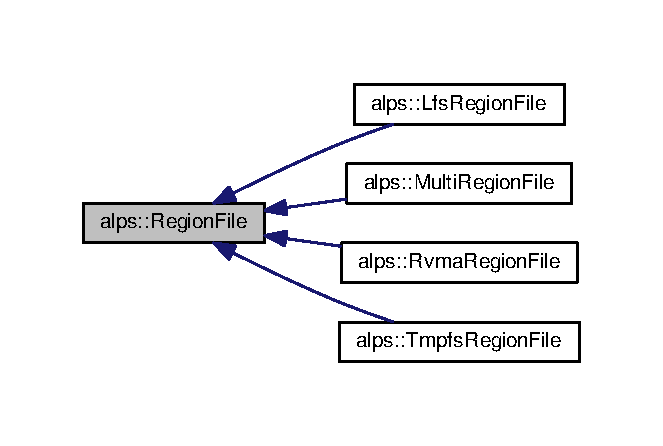
\includegraphics[width=318pt]{classalps_1_1RegionFile__inherit__graph}
\end{center}
\end{figure}
\subsection*{Public Member Functions}
\begin{DoxyCompactItemize}
\item 
virtual \hyperlink{group__ERRORCODES_ga6263a3c9a0b8d36aea21cdd835ac99fe}{Error\+Code} {\bfseries unlink} ()=0\hypertarget{classalps_1_1RegionFile_aebc5927a8ea77dd8b5e5dacade6caadb}{}\label{classalps_1_1RegionFile_aebc5927a8ea77dd8b5e5dacade6caadb}

\item 
virtual \hyperlink{group__ERRORCODES_ga6263a3c9a0b8d36aea21cdd835ac99fe}{Error\+Code} {\bfseries close} ()=0\hypertarget{classalps_1_1RegionFile_a8173d825ad1971a27f3c32063c5e3fae}{}\label{classalps_1_1RegionFile_a8173d825ad1971a27f3c32063c5e3fae}

\item 
virtual \hyperlink{group__ERRORCODES_ga6263a3c9a0b8d36aea21cdd835ac99fe}{Error\+Code} {\bfseries truncate} (loff\+\_\+t length)=0\hypertarget{classalps_1_1RegionFile_ac03917df3c8e74f7110b7c8226c69e6f}{}\label{classalps_1_1RegionFile_ac03917df3c8e74f7110b7c8226c69e6f}

\item 
virtual \hyperlink{group__ERRORCODES_ga6263a3c9a0b8d36aea21cdd835ac99fe}{Error\+Code} {\bfseries size} (loff\+\_\+t $\ast$length)=0\hypertarget{classalps_1_1RegionFile_a8ca8db1813b07d36eef4c04221724f47}{}\label{classalps_1_1RegionFile_a8ca8db1813b07d36eef4c04221724f47}

\item 
virtual \hyperlink{group__ERRORCODES_ga6263a3c9a0b8d36aea21cdd835ac99fe}{Error\+Code} {\bfseries map} (void $\ast$addr\+\_\+hint, size\+\_\+t length, int prot, int flags, loff\+\_\+t offset, void $\ast$$\ast$mapped\+\_\+addr)=0\hypertarget{classalps_1_1RegionFile_a10d615eb7caa3613f75bd36b62ccb5d8}{}\label{classalps_1_1RegionFile_a10d615eb7caa3613f75bd36b62ccb5d8}

\item 
virtual \hyperlink{group__ERRORCODES_ga6263a3c9a0b8d36aea21cdd835ac99fe}{Error\+Code} {\bfseries unmap} (void $\ast$addr, size\+\_\+t length)=0\hypertarget{classalps_1_1RegionFile_a0b116f89f3f3ff685d7b942e52f64cb5}{}\label{classalps_1_1RegionFile_a0b116f89f3f3ff685d7b942e52f64cb5}

\item 
virtual \hyperlink{group__ERRORCODES_ga6263a3c9a0b8d36aea21cdd835ac99fe}{Error\+Code} {\bfseries getxattr} (const char $\ast$name, void $\ast$value, size\+\_\+t size)=0\hypertarget{classalps_1_1RegionFile_a93bd994b1d794e52dae032bc1a61035d}{}\label{classalps_1_1RegionFile_a93bd994b1d794e52dae032bc1a61035d}

\item 
virtual \hyperlink{group__ERRORCODES_ga6263a3c9a0b8d36aea21cdd835ac99fe}{Error\+Code} {\bfseries setxattr} (const char $\ast$name, const void $\ast$value, size\+\_\+t size, int flags)=0\hypertarget{classalps_1_1RegionFile_a6f39ed54e11e78196fefdae39fe124cb}{}\label{classalps_1_1RegionFile_a6f39ed54e11e78196fefdae39fe124cb}

\item 
virtual size\+\_\+t {\bfseries booksize} ()=0\hypertarget{classalps_1_1RegionFile_aeaacd93f0bbb9fa9f0d27a7c743b91b5}{}\label{classalps_1_1RegionFile_aeaacd93f0bbb9fa9f0d27a7c743b91b5}

\item 
virtual \hyperlink{group__ERRORCODES_ga6263a3c9a0b8d36aea21cdd835ac99fe}{Error\+Code} {\bfseries create} (mode\+\_\+t mode)=0\hypertarget{classalps_1_1RegionFile_a5e8d30c5750eeda8d90778b57719a4e2}{}\label{classalps_1_1RegionFile_a5e8d30c5750eeda8d90778b57719a4e2}

\item 
virtual \hyperlink{group__ERRORCODES_ga6263a3c9a0b8d36aea21cdd835ac99fe}{Error\+Code} {\bfseries open} (int flags, mode\+\_\+t mode)=0\hypertarget{classalps_1_1RegionFile_af452bd729854c0ed2b37a7e18ce9b559}{}\label{classalps_1_1RegionFile_af452bd729854c0ed2b37a7e18ce9b559}

\item 
virtual \hyperlink{group__ERRORCODES_ga6263a3c9a0b8d36aea21cdd835ac99fe}{Error\+Code} {\bfseries open} (int flags)=0\hypertarget{classalps_1_1RegionFile_a906925033130d1fa0cc679b4d497c6e2}{}\label{classalps_1_1RegionFile_a906925033130d1fa0cc679b4d497c6e2}

\item 
virtual \hyperlink{group__ERRORCODES_ga6263a3c9a0b8d36aea21cdd835ac99fe}{Error\+Code} {\bfseries set\+\_\+interleave\+\_\+group} (loff\+\_\+t offset, loff\+\_\+t length, const std\+::vector$<$ Interleave\+Group $>$ \&vig)\hypertarget{classalps_1_1RegionFile_a6c291d58ef854587c8e50f6e3e3a8f88}{}\label{classalps_1_1RegionFile_a6c291d58ef854587c8e50f6e3e3a8f88}

\item 
virtual \hyperlink{group__ERRORCODES_ga6263a3c9a0b8d36aea21cdd835ac99fe}{Error\+Code} {\bfseries interleave\+\_\+group} (loff\+\_\+t offset, loff\+\_\+t length, std\+::vector$<$ Interleave\+Group $>$ $\ast$vig)\hypertarget{classalps_1_1RegionFile_a62642f3729211b7e02239f6d099ab3e8}{}\label{classalps_1_1RegionFile_a62642f3729211b7e02239f6d099ab3e8}

\end{DoxyCompactItemize}
\subsection*{Friends}
\begin{DoxyCompactItemize}
\item 
class {\bfseries Region\+File\+Factory}\hypertarget{classalps_1_1RegionFile_a76c88d2d08e2b3f7c7245690dfa65d84}{}\label{classalps_1_1RegionFile_a76c88d2d08e2b3f7c7245690dfa65d84}

\end{DoxyCompactItemize}


\subsection{Detailed Description}
This base class implements a common interface to region files backed by different types of memory file systems (e.\+g., T\+M\+P\+FS, L\+FS, E\+X\+T4+\+D\+AX). The A\+PI method names are self-\/described; they do what you expect them to do. 

The documentation for this class was generated from the following files\+:\begin{DoxyCompactItemize}
\item 
/home/yuan/\+Benchmarks/whisper/mnemosyne-\/gcc/usermode/library/pmalloc/include/alps/src/pegasus/region\+\_\+file.\+hh\item 
/home/yuan/\+Benchmarks/whisper/mnemosyne-\/gcc/usermode/library/pmalloc/include/alps/src/pegasus/region\+\_\+file.\+cc\end{DoxyCompactItemize}

\hypertarget{classalps_1_1RegionFileFactory}{}\section{alps\+:\+:Region\+File\+Factory Class Reference}
\label{classalps_1_1RegionFileFactory}\index{alps\+::\+Region\+File\+Factory@{alps\+::\+Region\+File\+Factory}}


\hyperlink{classalps_1_1Region}{Region} file factory.  




{\ttfamily \#include $<$region\+\_\+file\+\_\+factory.\+hh$>$}



Inheritance diagram for alps\+:\+:Region\+File\+Factory\+:
\nopagebreak
\begin{figure}[H]
\begin{center}
\leavevmode
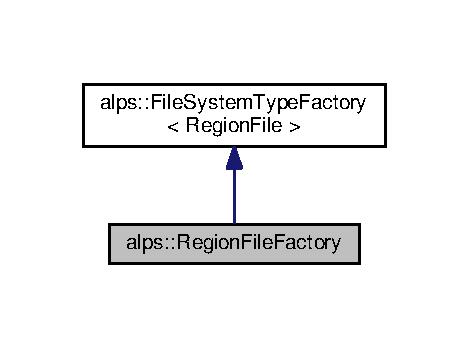
\includegraphics[width=225pt]{classalps_1_1RegionFileFactory__inherit__graph}
\end{center}
\end{figure}


Collaboration diagram for alps\+:\+:Region\+File\+Factory\+:
\nopagebreak
\begin{figure}[H]
\begin{center}
\leavevmode
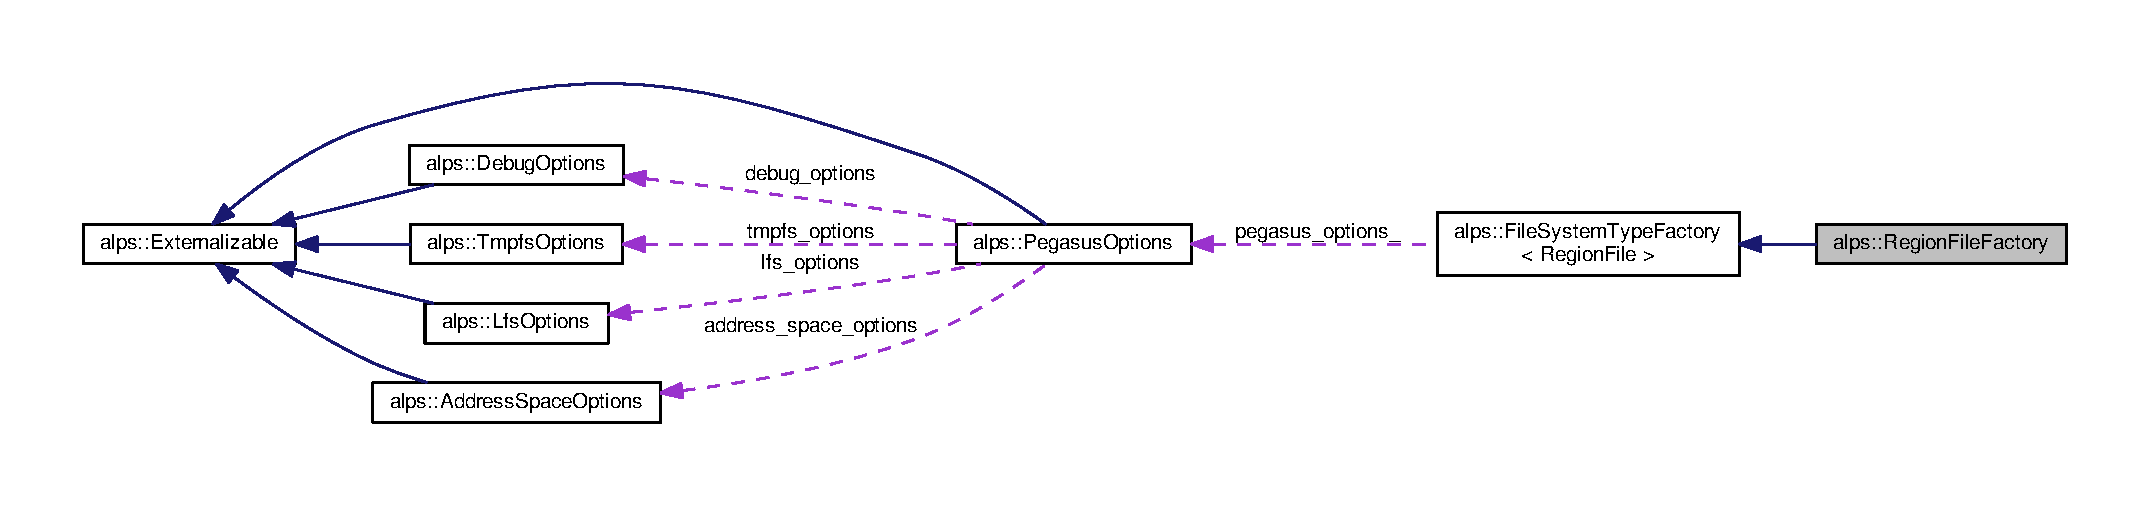
\includegraphics[width=350pt]{classalps_1_1RegionFileFactory__coll__graph}
\end{center}
\end{figure}
\subsection*{Public Member Functions}
\begin{DoxyCompactItemize}
\item 
{\bfseries Region\+File\+Factory} (const \hyperlink{structalps_1_1PegasusOptions}{Pegasus\+Options} \&pegasus\+\_\+options)\hypertarget{classalps_1_1RegionFileFactory_af2ad3418a86a40927c481801c2652292}{}\label{classalps_1_1RegionFileFactory_af2ad3418a86a40927c481801c2652292}

\item 
\hyperlink{group__ERRORCODES_ga6263a3c9a0b8d36aea21cdd835ac99fe}{Error\+Code} {\bfseries create} (const boost\+::filesystem\+::path \&pathname, mode\+\_\+t mode, \hyperlink{classalps_1_1RegionFile}{Region\+File} $\ast$$\ast$region\+\_\+file)\hypertarget{classalps_1_1RegionFileFactory_a554ff5b3f73e4ab1ee5ade21784d7f1d}{}\label{classalps_1_1RegionFileFactory_a554ff5b3f73e4ab1ee5ade21784d7f1d}

\item 
\hyperlink{group__ERRORCODES_ga6263a3c9a0b8d36aea21cdd835ac99fe}{Error\+Code} {\bfseries open} (const boost\+::filesystem\+::path \&pathname, int flags, mode\+\_\+t mode, \hyperlink{classalps_1_1RegionFile}{Region\+File} $\ast$$\ast$region\+\_\+file)\hypertarget{classalps_1_1RegionFileFactory_ab91c685d8ce59846ad5d2dda7e0a2c19}{}\label{classalps_1_1RegionFileFactory_ab91c685d8ce59846ad5d2dda7e0a2c19}

\item 
\hyperlink{group__ERRORCODES_ga6263a3c9a0b8d36aea21cdd835ac99fe}{Error\+Code} {\bfseries open} (const std\+::vector$<$ boost\+::filesystem\+::path $>$ \&pathnames, int flags, mode\+\_\+t mode, \hyperlink{classalps_1_1RegionFile}{Region\+File} $\ast$$\ast$region\+\_\+file)\hypertarget{classalps_1_1RegionFileFactory_ad22600e030b7ceb11ca8e2691aaf116f}{}\label{classalps_1_1RegionFileFactory_ad22600e030b7ceb11ca8e2691aaf116f}

\item 
\hyperlink{group__ERRORCODES_ga6263a3c9a0b8d36aea21cdd835ac99fe}{Error\+Code} {\bfseries open} (const boost\+::filesystem\+::path \&pathname, int flags, \hyperlink{classalps_1_1RegionFile}{Region\+File} $\ast$$\ast$region\+\_\+file)\hypertarget{classalps_1_1RegionFileFactory_ac9332016b8741a3121546a1db7a78f1e}{}\label{classalps_1_1RegionFileFactory_ac9332016b8741a3121546a1db7a78f1e}

\item 
\hyperlink{group__ERRORCODES_ga6263a3c9a0b8d36aea21cdd835ac99fe}{Error\+Code} {\bfseries open} (const std\+::vector$<$ boost\+::filesystem\+::path $>$ \&pathnames, int flags, \hyperlink{classalps_1_1RegionFile}{Region\+File} $\ast$$\ast$region\+\_\+file)\hypertarget{classalps_1_1RegionFileFactory_af3327449b61e0f316c0f6802d6863f48}{}\label{classalps_1_1RegionFileFactory_af3327449b61e0f316c0f6802d6863f48}

\end{DoxyCompactItemize}
\subsection*{Additional Inherited Members}


The documentation for this class was generated from the following files\+:\begin{DoxyCompactItemize}
\item 
/home/yuan/\+Benchmarks/whisper/mnemosyne-\/gcc/usermode/library/pmalloc/include/alps/src/pegasus/region\+\_\+file\+\_\+factory.\+hh\item 
/home/yuan/\+Benchmarks/whisper/mnemosyne-\/gcc/usermode/library/pmalloc/include/alps/src/pegasus/region\+\_\+file\+\_\+factory.\+cc\end{DoxyCompactItemize}

\hypertarget{classalps_1_1RvmaRegionFile}{}\section{alps\+:\+:Rvma\+Region\+File Class Reference}
\label{classalps_1_1RvmaRegionFile}\index{alps\+::\+Rvma\+Region\+File@{alps\+::\+Rvma\+Region\+File}}


Represents a region file backed by an R\+V\+MA context.  




{\ttfamily \#include $<$rvma\+\_\+region\+\_\+file.\+hh$>$}



Inheritance diagram for alps\+:\+:Rvma\+Region\+File\+:
\nopagebreak
\begin{figure}[H]
\begin{center}
\leavevmode
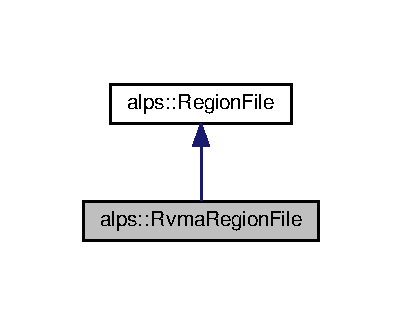
\includegraphics[width=193pt]{classalps_1_1RvmaRegionFile__inherit__graph}
\end{center}
\end{figure}


Collaboration diagram for alps\+:\+:Rvma\+Region\+File\+:
\nopagebreak
\begin{figure}[H]
\begin{center}
\leavevmode
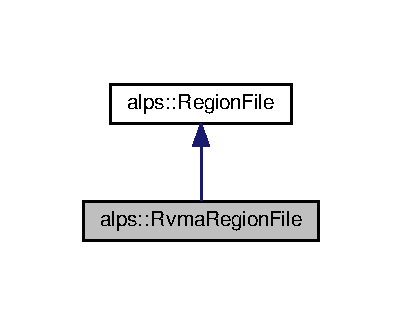
\includegraphics[width=193pt]{classalps_1_1RvmaRegionFile__coll__graph}
\end{center}
\end{figure}
\subsection*{Additional Inherited Members}


The documentation for this class was generated from the following file\+:\begin{DoxyCompactItemize}
\item 
/home/yuan/\+Benchmarks/whisper/mnemosyne-\/gcc/usermode/library/pmalloc/include/alps/src/pegasus/rvma\+\_\+region\+\_\+file.\+hh\end{DoxyCompactItemize}

\hypertarget{structalps_1_1TmpfsOptions}{}\section{alps\+:\+:Tmpfs\+Options Struct Reference}
\label{structalps_1_1TmpfsOptions}\index{alps\+::\+Tmpfs\+Options@{alps\+::\+Tmpfs\+Options}}


Inheritance diagram for alps\+:\+:Tmpfs\+Options\+:
\nopagebreak
\begin{figure}[H]
\begin{center}
\leavevmode
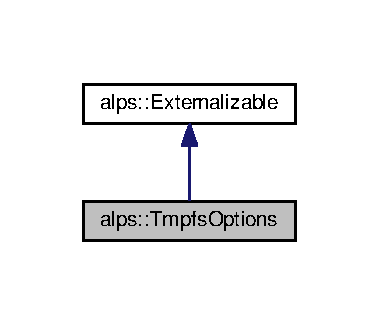
\includegraphics[width=182pt]{structalps_1_1TmpfsOptions__inherit__graph}
\end{center}
\end{figure}


Collaboration diagram for alps\+:\+:Tmpfs\+Options\+:
\nopagebreak
\begin{figure}[H]
\begin{center}
\leavevmode
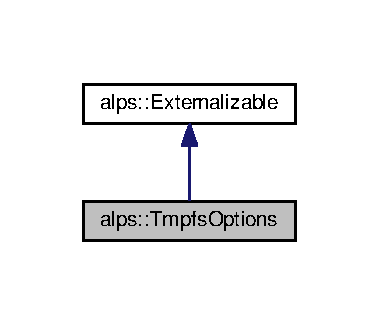
\includegraphics[width=182pt]{structalps_1_1TmpfsOptions__coll__graph}
\end{center}
\end{figure}
\subsection*{Public Member Functions}
\begin{DoxyCompactItemize}
\item 
\hyperlink{structalps_1_1TmpfsOptions_aa7d24ac1be4e5bcc6822f5ea1753cc3c}{Tmpfs\+Options} ()
\end{DoxyCompactItemize}
\subsection*{Public Attributes}
\begin{DoxyCompactItemize}
\item 
std\+::size\+\_\+t {\bfseries k\+Default\+Book\+Size\+Bytes} = 8$\ast$1024$\ast$1024\+L\+LU\hypertarget{structalps_1_1TmpfsOptions_acf0c8a74bbfd88362a9e595de243d8c4}{}\label{structalps_1_1TmpfsOptions_acf0c8a74bbfd88362a9e595de243d8c4}

\item 
size\+\_\+t {\bfseries book\+\_\+size\+\_\+bytes}\hypertarget{structalps_1_1TmpfsOptions_a4f3236bc82f39ed235455d64c23a094d}{}\label{structalps_1_1TmpfsOptions_a4f3236bc82f39ed235455d64c23a094d}

\end{DoxyCompactItemize}
\subsection*{Additional Inherited Members}


\subsection{Constructor \& Destructor Documentation}
\index{alps\+::\+Tmpfs\+Options@{alps\+::\+Tmpfs\+Options}!Tmpfs\+Options@{Tmpfs\+Options}}
\index{Tmpfs\+Options@{Tmpfs\+Options}!alps\+::\+Tmpfs\+Options@{alps\+::\+Tmpfs\+Options}}
\subsubsection[{\texorpdfstring{Tmpfs\+Options()}{TmpfsOptions()}}]{\setlength{\rightskip}{0pt plus 5cm}alps\+::\+Tmpfs\+Options\+::\+Tmpfs\+Options (
\begin{DoxyParamCaption}
{}
\end{DoxyParamCaption}
)\hspace{0.3cm}{\ttfamily [inline]}}\hypertarget{structalps_1_1TmpfsOptions_aa7d24ac1be4e5bcc6822f5ea1753cc3c}{}\label{structalps_1_1TmpfsOptions_aa7d24ac1be4e5bcc6822f5ea1753cc3c}
Constructs option values with default values 

The documentation for this struct was generated from the following file\+:\begin{DoxyCompactItemize}
\item 
/home/yuan/\+Benchmarks/whisper/mnemosyne-\/gcc/usermode/library/pmalloc/include/alps/include/alps/pegasus/tmpfs\+\_\+options.\+hh\end{DoxyCompactItemize}

\hypertarget{classalps_1_1TmpfsRegionFile}{}\section{alps\+:\+:Tmpfs\+Region\+File Class Reference}
\label{classalps_1_1TmpfsRegionFile}\index{alps\+::\+Tmpfs\+Region\+File@{alps\+::\+Tmpfs\+Region\+File}}


Represents a region file backed by T\+M\+P\+FS.  




{\ttfamily \#include $<$tmpfs\+\_\+region\+\_\+file.\+hh$>$}



Inheritance diagram for alps\+:\+:Tmpfs\+Region\+File\+:
\nopagebreak
\begin{figure}[H]
\begin{center}
\leavevmode
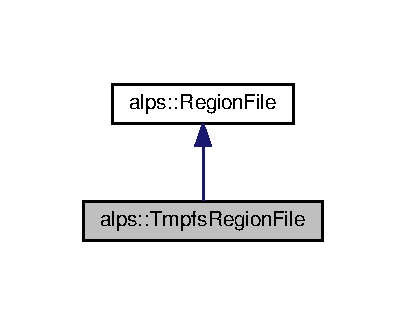
\includegraphics[width=195pt]{classalps_1_1TmpfsRegionFile__inherit__graph}
\end{center}
\end{figure}


Collaboration diagram for alps\+:\+:Tmpfs\+Region\+File\+:
\nopagebreak
\begin{figure}[H]
\begin{center}
\leavevmode
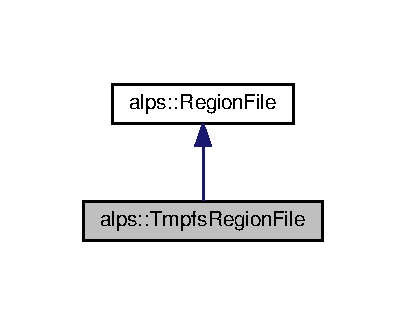
\includegraphics[width=195pt]{classalps_1_1TmpfsRegionFile__coll__graph}
\end{center}
\end{figure}
\subsection*{Public Types}
\begin{DoxyCompactItemize}
\item 
enum {\bfseries Interleave\+Policy} \{ {\bfseries k\+Precise\+Allocate} = 0, 
{\bfseries k\+Round\+Robin}
 \}\hypertarget{classalps_1_1TmpfsRegionFile_a4c77cd5eea6561a439c3e0507428864a}{}\label{classalps_1_1TmpfsRegionFile_a4c77cd5eea6561a439c3e0507428864a}

\end{DoxyCompactItemize}
\subsection*{Public Member Functions}
\begin{DoxyCompactItemize}
\item 
{\bfseries Tmpfs\+Region\+File} (boost\+::filesystem\+::path pathname, boost\+::filesystem\+::path xpathname, const \hyperlink{structalps_1_1PegasusOptions}{Pegasus\+Options} \&pegasus\+\_\+options)\hypertarget{classalps_1_1TmpfsRegionFile_a64efd95e0f04958b38848f00ba625398}{}\label{classalps_1_1TmpfsRegionFile_a64efd95e0f04958b38848f00ba625398}

\item 
\hyperlink{group__ERRORCODES_ga6263a3c9a0b8d36aea21cdd835ac99fe}{Error\+Code} {\bfseries create} (mode\+\_\+t mode)\hypertarget{classalps_1_1TmpfsRegionFile_af056c20aaaba28a3773c86e00978dfef}{}\label{classalps_1_1TmpfsRegionFile_af056c20aaaba28a3773c86e00978dfef}

\item 
\hyperlink{group__ERRORCODES_ga6263a3c9a0b8d36aea21cdd835ac99fe}{Error\+Code} {\bfseries open} (int flags, mode\+\_\+t mode)\hypertarget{classalps_1_1TmpfsRegionFile_a2d41f9debc39a99d4dc8d3dd8829fb14}{}\label{classalps_1_1TmpfsRegionFile_a2d41f9debc39a99d4dc8d3dd8829fb14}

\item 
\hyperlink{group__ERRORCODES_ga6263a3c9a0b8d36aea21cdd835ac99fe}{Error\+Code} {\bfseries open} (int flags)\hypertarget{classalps_1_1TmpfsRegionFile_afe41df2a968e570755ff6053e1d50836}{}\label{classalps_1_1TmpfsRegionFile_afe41df2a968e570755ff6053e1d50836}

\item 
\hyperlink{group__ERRORCODES_ga6263a3c9a0b8d36aea21cdd835ac99fe}{Error\+Code} {\bfseries unlink} ()\hypertarget{classalps_1_1TmpfsRegionFile_a47210b5f2e7af168672fa36e845bf4fa}{}\label{classalps_1_1TmpfsRegionFile_a47210b5f2e7af168672fa36e845bf4fa}

\item 
\hyperlink{group__ERRORCODES_ga6263a3c9a0b8d36aea21cdd835ac99fe}{Error\+Code} {\bfseries close} ()\hypertarget{classalps_1_1TmpfsRegionFile_a3823425d2b9d276066a66ef09eadea7b}{}\label{classalps_1_1TmpfsRegionFile_a3823425d2b9d276066a66ef09eadea7b}

\item 
\hyperlink{group__ERRORCODES_ga6263a3c9a0b8d36aea21cdd835ac99fe}{Error\+Code} {\bfseries truncate} (loff\+\_\+t length)\hypertarget{classalps_1_1TmpfsRegionFile_af5c68479c8c306464ef9a6ac936d7e16}{}\label{classalps_1_1TmpfsRegionFile_af5c68479c8c306464ef9a6ac936d7e16}

\item 
\hyperlink{group__ERRORCODES_ga6263a3c9a0b8d36aea21cdd835ac99fe}{Error\+Code} {\bfseries size} (loff\+\_\+t $\ast$length)\hypertarget{classalps_1_1TmpfsRegionFile_a3595a7f5562fb4979dcc8d0e3a527b0d}{}\label{classalps_1_1TmpfsRegionFile_a3595a7f5562fb4979dcc8d0e3a527b0d}

\item 
\hyperlink{group__ERRORCODES_ga6263a3c9a0b8d36aea21cdd835ac99fe}{Error\+Code} {\bfseries map} (void $\ast$addr\+\_\+hint, size\+\_\+t length, int prot, int flags, loff\+\_\+t offset, void $\ast$$\ast$mapped\+\_\+addr)\hypertarget{classalps_1_1TmpfsRegionFile_aecbcd4faa44978e67c2c035ad625f50f}{}\label{classalps_1_1TmpfsRegionFile_aecbcd4faa44978e67c2c035ad625f50f}

\item 
\hyperlink{group__ERRORCODES_ga6263a3c9a0b8d36aea21cdd835ac99fe}{Error\+Code} {\bfseries unmap} (void $\ast$addr, size\+\_\+t length)\hypertarget{classalps_1_1TmpfsRegionFile_ad1239e1fbf298cf231eaab669804a969}{}\label{classalps_1_1TmpfsRegionFile_ad1239e1fbf298cf231eaab669804a969}

\item 
\hyperlink{group__ERRORCODES_ga6263a3c9a0b8d36aea21cdd835ac99fe}{Error\+Code} {\bfseries getxattr} (const char $\ast$name, void $\ast$value, size\+\_\+t size)\hypertarget{classalps_1_1TmpfsRegionFile_ac9ff7ea5c734c98a6e083350c17acf54}{}\label{classalps_1_1TmpfsRegionFile_ac9ff7ea5c734c98a6e083350c17acf54}

\item 
\hyperlink{group__ERRORCODES_ga6263a3c9a0b8d36aea21cdd835ac99fe}{Error\+Code} {\bfseries setxattr} (const char $\ast$name, const void $\ast$value, size\+\_\+t size, int flags)\hypertarget{classalps_1_1TmpfsRegionFile_af122bc9e41a0ad54b3148999c61db27e}{}\label{classalps_1_1TmpfsRegionFile_af122bc9e41a0ad54b3148999c61db27e}

\item 
size\+\_\+t {\bfseries booksize} ()\hypertarget{classalps_1_1TmpfsRegionFile_acff37cfb3764b1d9bd889bd15f95b884}{}\label{classalps_1_1TmpfsRegionFile_acff37cfb3764b1d9bd889bd15f95b884}

\end{DoxyCompactItemize}
\subsection*{Static Public Member Functions}
\begin{DoxyCompactItemize}
\item 
static \hyperlink{classalps_1_1RegionFile}{Region\+File} $\ast$ {\bfseries construct} (const boost\+::filesystem\+::path \&pathname, const \hyperlink{structalps_1_1PegasusOptions}{Pegasus\+Options} \&pegasus\+\_\+options)\hypertarget{classalps_1_1TmpfsRegionFile_a7bf70ed90d3632cac14e8238d81fd57c}{}\label{classalps_1_1TmpfsRegionFile_a7bf70ed90d3632cac14e8238d81fd57c}

\end{DoxyCompactItemize}
\subsection*{Static Public Attributes}
\begin{DoxyCompactItemize}
\item 
static const char $\ast$ {\bfseries k\+Lock\+File\+Name} = \char`\"{}/dev/shm/@@lockfile@@\char`\"{}\hypertarget{classalps_1_1TmpfsRegionFile_a95e31e53958f0fb9e6989bfd4f4c33c6}{}\label{classalps_1_1TmpfsRegionFile_a95e31e53958f0fb9e6989bfd4f4c33c6}

\item 
static const char $\ast$ {\bfseries k\+Xattr\+Extension} = \char`\"{}.xattr\char`\"{}\hypertarget{classalps_1_1TmpfsRegionFile_a41052c07862762ae01b6dde6aea3c1d7}{}\label{classalps_1_1TmpfsRegionFile_a41052c07862762ae01b6dde6aea3c1d7}

\item 
static Interleave\+Policy {\bfseries interleave\+\_\+policy\+\_\+} = Tmpfs\+Region\+File\+::k\+Precise\+Allocate\hypertarget{classalps_1_1TmpfsRegionFile_a0ba492a78a1ea43617083b958ef61ab6}{}\label{classalps_1_1TmpfsRegionFile_a0ba492a78a1ea43617083b958ef61ab6}

\end{DoxyCompactItemize}


The documentation for this class was generated from the following files\+:\begin{DoxyCompactItemize}
\item 
/home/yuan/\+Benchmarks/whisper/mnemosyne-\/gcc/usermode/library/pmalloc/include/alps/src/pegasus/tmpfs\+\_\+region\+\_\+file.\+hh\item 
/home/yuan/\+Benchmarks/whisper/mnemosyne-\/gcc/usermode/library/pmalloc/include/alps/src/pegasus/tmpfs\+\_\+region\+\_\+file.\+cc\end{DoxyCompactItemize}

\hypertarget{classalps_1_1TmpfsTopology}{}\section{alps\+:\+:Tmpfs\+Topology Class Reference}
\label{classalps_1_1TmpfsTopology}\index{alps\+::\+Tmpfs\+Topology@{alps\+::\+Tmpfs\+Topology}}


Inheritance diagram for alps\+:\+:Tmpfs\+Topology\+:
\nopagebreak
\begin{figure}[H]
\begin{center}
\leavevmode
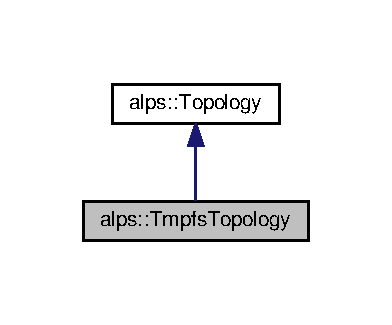
\includegraphics[width=188pt]{classalps_1_1TmpfsTopology__inherit__graph}
\end{center}
\end{figure}


Collaboration diagram for alps\+:\+:Tmpfs\+Topology\+:
\nopagebreak
\begin{figure}[H]
\begin{center}
\leavevmode
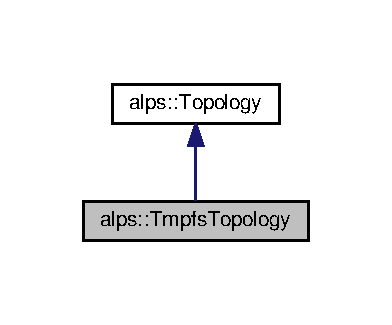
\includegraphics[width=188pt]{classalps_1_1TmpfsTopology__coll__graph}
\end{center}
\end{figure}
\subsection*{Public Member Functions}
\begin{DoxyCompactItemize}
\item 
{\bfseries Tmpfs\+Topology} (const boost\+::filesystem\+::path \&path, const \hyperlink{structalps_1_1PegasusOptions}{Pegasus\+Options} \&pegasus\+\_\+options)\hypertarget{classalps_1_1TmpfsTopology_ab9b305dc0370c5dbd8ca37c29aab4c1d}{}\label{classalps_1_1TmpfsTopology_ab9b305dc0370c5dbd8ca37c29aab4c1d}

\item 
Interleave\+Group \hyperlink{classalps_1_1TmpfsTopology_a1f4313dce7095500979318dcf754de04}{max\+\_\+interleave\+\_\+group} ()\hypertarget{classalps_1_1TmpfsTopology_a1f4313dce7095500979318dcf754de04}{}\label{classalps_1_1TmpfsTopology_a1f4313dce7095500979318dcf754de04}

\begin{DoxyCompactList}\small\item\em Returns the highest node number available in the system. \end{DoxyCompactList}\item 
Interleave\+Group \hyperlink{classalps_1_1TmpfsTopology_aff12311096104e9bcecaeabcb1bd7196}{nearest\+\_\+ig} ()\hypertarget{classalps_1_1TmpfsTopology_aff12311096104e9bcecaeabcb1bd7196}{}\label{classalps_1_1TmpfsTopology_aff12311096104e9bcecaeabcb1bd7196}

\begin{DoxyCompactList}\small\item\em Returns the nearest interleave group to the node the calling process is running on. \end{DoxyCompactList}\item 
int {\bfseries run\+\_\+on\+\_\+node} (int n)\hypertarget{classalps_1_1TmpfsTopology_ae1eae1973cee1120293686752cfb3129}{}\label{classalps_1_1TmpfsTopology_ae1eae1973cee1120293686752cfb3129}

\end{DoxyCompactItemize}
\subsection*{Static Public Member Functions}
\begin{DoxyCompactItemize}
\item 
static \hyperlink{classalps_1_1Topology}{Topology} $\ast$ {\bfseries construct} (const boost\+::filesystem\+::path \&pathname, const \hyperlink{structalps_1_1PegasusOptions}{Pegasus\+Options} \&pegasus\+\_\+options)\hypertarget{classalps_1_1TmpfsTopology_adedbd94b4c01dbdddb0241b276068145}{}\label{classalps_1_1TmpfsTopology_adedbd94b4c01dbdddb0241b276068145}

\end{DoxyCompactItemize}


The documentation for this class was generated from the following files\+:\begin{DoxyCompactItemize}
\item 
/home/yuan/\+Benchmarks/whisper/mnemosyne-\/gcc/usermode/library/pmalloc/include/alps/src/pegasus/tmpfs\+\_\+topology.\+hh\item 
/home/yuan/\+Benchmarks/whisper/mnemosyne-\/gcc/usermode/library/pmalloc/include/alps/src/pegasus/tmpfs\+\_\+topology.\+cc\end{DoxyCompactItemize}

\hypertarget{classalps_1_1Topology}{}\section{alps\+:\+:Topology Class Reference}
\label{classalps_1_1Topology}\index{alps\+::\+Topology@{alps\+::\+Topology}}


Inheritance diagram for alps\+:\+:Topology\+:
\nopagebreak
\begin{figure}[H]
\begin{center}
\leavevmode
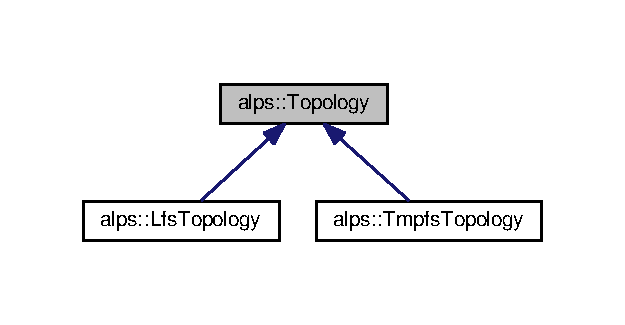
\includegraphics[width=300pt]{classalps_1_1Topology__inherit__graph}
\end{center}
\end{figure}
\subsection*{Public Member Functions}
\begin{DoxyCompactItemize}
\item 
virtual Interleave\+Group \hyperlink{classalps_1_1Topology_a90b74887b475e671e36910e5d558d169}{max\+\_\+interleave\+\_\+group} ()=0\hypertarget{classalps_1_1Topology_a90b74887b475e671e36910e5d558d169}{}\label{classalps_1_1Topology_a90b74887b475e671e36910e5d558d169}

\begin{DoxyCompactList}\small\item\em Returns the highest node number available in the system. \end{DoxyCompactList}\item 
virtual Interleave\+Group \hyperlink{classalps_1_1Topology_a213696634a781fa24f8f1b69f1c782e0}{nearest\+\_\+ig} ()=0\hypertarget{classalps_1_1Topology_a213696634a781fa24f8f1b69f1c782e0}{}\label{classalps_1_1Topology_a213696634a781fa24f8f1b69f1c782e0}

\begin{DoxyCompactList}\small\item\em Returns the nearest interleave group to the node the calling process is running on. \end{DoxyCompactList}\end{DoxyCompactItemize}


The documentation for this class was generated from the following files\+:\begin{DoxyCompactItemize}
\item 
/home/yuan/\+Benchmarks/whisper/mnemosyne-\/gcc/usermode/library/pmalloc/include/alps/src/pegasus/topology.\+hh\item 
/home/yuan/\+Benchmarks/whisper/mnemosyne-\/gcc/usermode/library/pmalloc/include/alps/src/pegasus/topology.\+cc\end{DoxyCompactItemize}

\hypertarget{classalps_1_1TopologyFactory}{}\section{alps\+:\+:Topology\+Factory Class Reference}
\label{classalps_1_1TopologyFactory}\index{alps\+::\+Topology\+Factory@{alps\+::\+Topology\+Factory}}


Inheritance diagram for alps\+:\+:Topology\+Factory\+:
\nopagebreak
\begin{figure}[H]
\begin{center}
\leavevmode
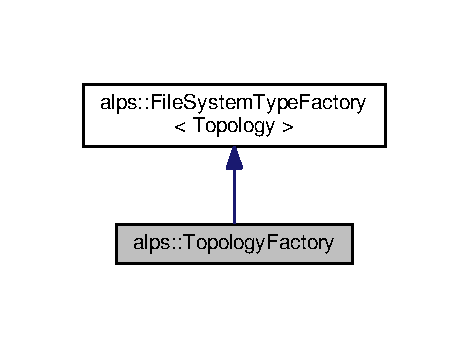
\includegraphics[width=225pt]{classalps_1_1TopologyFactory__inherit__graph}
\end{center}
\end{figure}


Collaboration diagram for alps\+:\+:Topology\+Factory\+:
\nopagebreak
\begin{figure}[H]
\begin{center}
\leavevmode
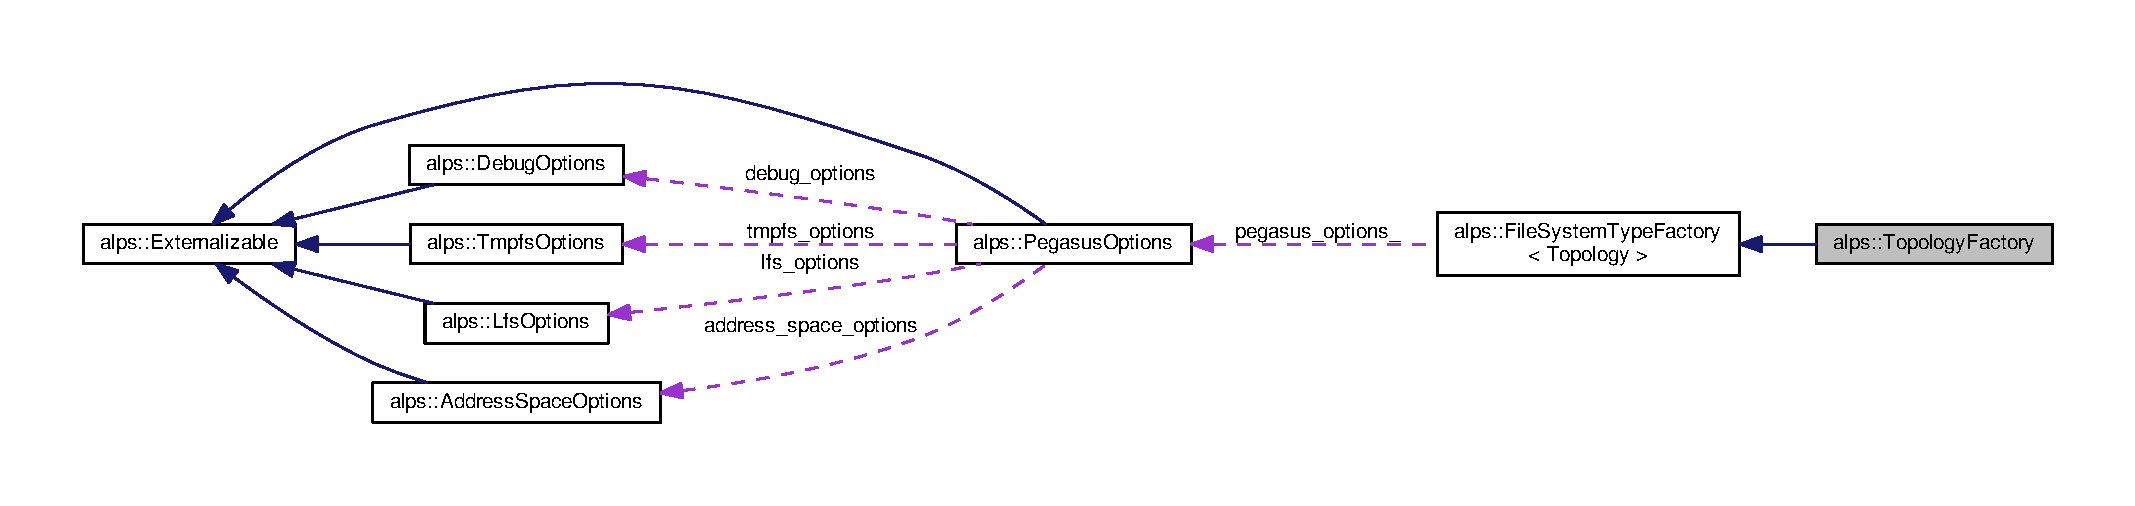
\includegraphics[width=350pt]{classalps_1_1TopologyFactory__coll__graph}
\end{center}
\end{figure}
\subsection*{Public Member Functions}
\begin{DoxyCompactItemize}
\item 
{\bfseries Topology\+Factory} (const \hyperlink{structalps_1_1PegasusOptions}{Pegasus\+Options} \&pegasus\+\_\+options)\hypertarget{classalps_1_1TopologyFactory_a7593660e90292efe41e14d8ac4095a4c}{}\label{classalps_1_1TopologyFactory_a7593660e90292efe41e14d8ac4095a4c}

\end{DoxyCompactItemize}
\subsection*{Additional Inherited Members}


The documentation for this class was generated from the following file\+:\begin{DoxyCompactItemize}
\item 
/home/yuan/\+Benchmarks/whisper/mnemosyne-\/gcc/usermode/library/pmalloc/include/alps/src/pegasus/topology\+\_\+factory.\+hh\end{DoxyCompactItemize}

\hypertarget{classalps_1_1BaseRelativePointer_1_1TPtr}{}\section{alps\+:\+:Base\+Relative\+Pointer\+:\+:T\+Ptr$<$ Region\+Type, Pointed\+Type $>$ Class Template Reference}
\label{classalps_1_1BaseRelativePointer_1_1TPtr}\index{alps\+::\+Base\+Relative\+Pointer\+::\+T\+Ptr$<$ Region\+Type, Pointed\+Type $>$@{alps\+::\+Base\+Relative\+Pointer\+::\+T\+Ptr$<$ Region\+Type, Pointed\+Type $>$}}


Represents a transient pointer.  




{\ttfamily \#include $<$pointer.\+hh$>$}



Collaboration diagram for alps\+:\+:Base\+Relative\+Pointer\+:\+:T\+Ptr$<$ Region\+Type, Pointed\+Type $>$\+:
\nopagebreak
\begin{figure}[H]
\begin{center}
\leavevmode
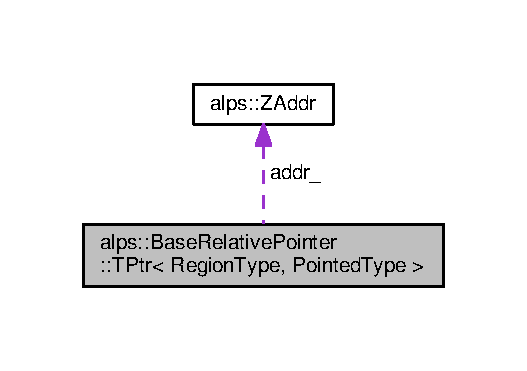
\includegraphics[width=253pt]{classalps_1_1BaseRelativePointer_1_1TPtr__coll__graph}
\end{center}
\end{figure}
\subsection*{Public Types}
\begin{DoxyCompactItemize}
\item 
typedef Pointed\+Type $\ast$ {\bfseries pointer}\hypertarget{classalps_1_1BaseRelativePointer_1_1TPtr_a540d6b534b74d35f28153c81ed6dec57}{}\label{classalps_1_1BaseRelativePointer_1_1TPtr_a540d6b534b74d35f28153c81ed6dec57}

\item 
typedef boost\+::add\+\_\+reference$<$ Pointed\+Type $>$\+::type {\bfseries reference}\hypertarget{classalps_1_1BaseRelativePointer_1_1TPtr_a93313c9c52b5b26d6fb333d4370fce98}{}\label{classalps_1_1BaseRelativePointer_1_1TPtr_a93313c9c52b5b26d6fb333d4370fce98}

\end{DoxyCompactItemize}
\subsection*{Public Member Functions}
\begin{DoxyCompactItemize}
\item 
{\bfseries T\+Ptr} (\hyperlink{structalps_1_1ZAddr}{Z\+Addr} zaddr)\hypertarget{classalps_1_1BaseRelativePointer_1_1TPtr_a10ab6fccc1914483537708bfbdd0876b}{}\label{classalps_1_1BaseRelativePointer_1_1TPtr_a10ab6fccc1914483537708bfbdd0876b}

\item 
{\bfseries T\+Ptr} (Region\+Id region\+\_\+id, Linear\+Addr offset)\hypertarget{classalps_1_1BaseRelativePointer_1_1TPtr_a8af8b7b46e5fc2a8d0a6482531374072}{}\label{classalps_1_1BaseRelativePointer_1_1TPtr_a8af8b7b46e5fc2a8d0a6482531374072}

\item 
{\bfseries T\+Ptr} (Region\+Type $\ast$pregion, Linear\+Addr offset)\hypertarget{classalps_1_1BaseRelativePointer_1_1TPtr_af6c3c509d387efba87e5a824ab9ef54d}{}\label{classalps_1_1BaseRelativePointer_1_1TPtr_af6c3c509d387efba87e5a824ab9ef54d}

\item 
{\bfseries T\+Ptr} (const \hyperlink{classalps_1_1BaseRelativePointer_1_1TPtr}{T\+Ptr}$<$ Region\+Type, void $>$ \&other)\hypertarget{classalps_1_1BaseRelativePointer_1_1TPtr_a6a3c95e7f917ce78d53f912a116d7fdf}{}\label{classalps_1_1BaseRelativePointer_1_1TPtr_a6a3c95e7f917ce78d53f912a116d7fdf}

\item 
{\bfseries T\+Ptr} (const \hyperlink{classalps_1_1BaseRelativePointer_1_1IPtr}{I\+Ptr}$<$ Region\+Type, Pointed\+Type $>$ \&other)\hypertarget{classalps_1_1BaseRelativePointer_1_1TPtr_a7c7a365923f356bceeefc09d0238ba4e}{}\label{classalps_1_1BaseRelativePointer_1_1TPtr_a7c7a365923f356bceeefc09d0238ba4e}

\item 
{\bfseries T\+Ptr} (Pointed\+Type $\ast$from)\hypertarget{classalps_1_1BaseRelativePointer_1_1TPtr_aa1ed21917a029238fab18ed44d81ceea}{}\label{classalps_1_1BaseRelativePointer_1_1TPtr_aa1ed21917a029238fab18ed44d81ceea}

\item 
{\bfseries operator I\+Ptr$<$ Region\+Type, Pointed\+Type $>$} () const \hypertarget{classalps_1_1BaseRelativePointer_1_1TPtr_a815426f265c22440ae505346569bfee9}{}\label{classalps_1_1BaseRelativePointer_1_1TPtr_a815426f265c22440ae505346569bfee9}

\item 
\hyperlink{classalps_1_1BaseRelativePointer_1_1TPtr}{T\+Ptr} \& {\bfseries operator=} (const \hyperlink{classalps_1_1BaseRelativePointer_1_1IPtr}{I\+Ptr}$<$ Region\+Type, Pointed\+Type $>$ \&other)\hypertarget{classalps_1_1BaseRelativePointer_1_1TPtr_a868c62ae1ca78448451fffaace02a6d2}{}\label{classalps_1_1BaseRelativePointer_1_1TPtr_a868c62ae1ca78448451fffaace02a6d2}

\item 
\hyperlink{classalps_1_1BaseRelativePointer_1_1TPtr}{T\+Ptr} \& {\bfseries operator=} (const typename Region\+Type\+::template \hyperlink{classalps_1_1BaseRelativePointer_1_1TPtr}{T\+Ptr}$<$ Pointed\+Type $>$ \&tptr)\hypertarget{classalps_1_1BaseRelativePointer_1_1TPtr_a915e02d4d8de6f209e00ae0afb562ae5}{}\label{classalps_1_1BaseRelativePointer_1_1TPtr_a915e02d4d8de6f209e00ae0afb562ae5}

\item 
\hyperlink{classalps_1_1BaseRelativePointer_1_1TPtr}{T\+Ptr} \& {\bfseries operator=} (Pointed\+Type $\ast$from)\hypertarget{classalps_1_1BaseRelativePointer_1_1TPtr_a2e95d9beb43202b8152679bf66c4eb48}{}\label{classalps_1_1BaseRelativePointer_1_1TPtr_a2e95d9beb43202b8152679bf66c4eb48}

\item 
bool {\bfseries operator==} (const \hyperlink{structalps_1_1ZAddr}{Z\+Addr} \&other\+\_\+zaddr) const \hypertarget{classalps_1_1BaseRelativePointer_1_1TPtr_ab1c67178ed0369619c073bae4f19b4c3}{}\label{classalps_1_1BaseRelativePointer_1_1TPtr_ab1c67178ed0369619c073bae4f19b4c3}

\item 
bool {\bfseries operator!=} (const \hyperlink{structalps_1_1ZAddr}{Z\+Addr} \&other\+\_\+zaddr) const \hypertarget{classalps_1_1BaseRelativePointer_1_1TPtr_a4ada056e052fd9091728502b88a58a51}{}\label{classalps_1_1BaseRelativePointer_1_1TPtr_a4ada056e052fd9091728502b88a58a51}

\item 
{\bfseries operator Z\+Addr} () const \hypertarget{classalps_1_1BaseRelativePointer_1_1TPtr_abcdb8e7edc740d33431e61d9037ab876}{}\label{classalps_1_1BaseRelativePointer_1_1TPtr_abcdb8e7edc740d33431e61d9037ab876}

\item 
pointer {\bfseries get} () const \hypertarget{classalps_1_1BaseRelativePointer_1_1TPtr_a7d9dfb9e65407fb638675360ec4ca575}{}\label{classalps_1_1BaseRelativePointer_1_1TPtr_a7d9dfb9e65407fb638675360ec4ca575}

\item 
Region\+Id {\bfseries region\+\_\+id} () const \hypertarget{classalps_1_1BaseRelativePointer_1_1TPtr_a69b71f19f5a1d7ce2443b81220ffc672}{}\label{classalps_1_1BaseRelativePointer_1_1TPtr_a69b71f19f5a1d7ce2443b81220ffc672}

\item 
Linear\+Addr {\bfseries offset} () const \hypertarget{classalps_1_1BaseRelativePointer_1_1TPtr_a506f9ece88e3ff88e924fb226e41f475}{}\label{classalps_1_1BaseRelativePointer_1_1TPtr_a506f9ece88e3ff88e924fb226e41f475}

\item 
Region\+Type $\ast$ {\bfseries region} ()\hypertarget{classalps_1_1BaseRelativePointer_1_1TPtr_a9f3b32ad14fa72be97209a61a4ee39f9}{}\label{classalps_1_1BaseRelativePointer_1_1TPtr_a9f3b32ad14fa72be97209a61a4ee39f9}

\item 
pointer {\bfseries operator-\/$>$} () const \hypertarget{classalps_1_1BaseRelativePointer_1_1TPtr_a6dbaac6ffb3b1a815095e20b5a19abbb}{}\label{classalps_1_1BaseRelativePointer_1_1TPtr_a6dbaac6ffb3b1a815095e20b5a19abbb}

\item 
reference {\bfseries operator$\ast$} () const \hypertarget{classalps_1_1BaseRelativePointer_1_1TPtr_ae2edaf75f2ed04a77ea6b3a1c6ab1252}{}\label{classalps_1_1BaseRelativePointer_1_1TPtr_ae2edaf75f2ed04a77ea6b3a1c6ab1252}

\item 
bool {\bfseries operator$<$} (const \hyperlink{classalps_1_1BaseRelativePointer_1_1TPtr}{T\+Ptr} rhs) const \hypertarget{classalps_1_1BaseRelativePointer_1_1TPtr_ae0e5debc055d47038ce34fddb05c5651}{}\label{classalps_1_1BaseRelativePointer_1_1TPtr_ae0e5debc055d47038ce34fddb05c5651}

\item 
reference {\bfseries operator\mbox{[}$\,$\mbox{]}} (std\+::ptrdiff\+\_\+t idx) const \hypertarget{classalps_1_1BaseRelativePointer_1_1TPtr_a342ae6b7bbfdfd65eedc732ba9602aed}{}\label{classalps_1_1BaseRelativePointer_1_1TPtr_a342ae6b7bbfdfd65eedc732ba9602aed}

\item 
void {\bfseries inc\+\_\+offset} (std\+::ptrdiff\+\_\+t bytes)\hypertarget{classalps_1_1BaseRelativePointer_1_1TPtr_abf02b22701c1390cd38f3ca93f3cc2f3}{}\label{classalps_1_1BaseRelativePointer_1_1TPtr_abf02b22701c1390cd38f3ca93f3cc2f3}

\item 
void {\bfseries dec\+\_\+offset} (std\+::ptrdiff\+\_\+t bytes)\hypertarget{classalps_1_1BaseRelativePointer_1_1TPtr_ab61c461db2fb60f93220b42987cef6c3}{}\label{classalps_1_1BaseRelativePointer_1_1TPtr_ab61c461db2fb60f93220b42987cef6c3}

\item 
\hyperlink{classalps_1_1BaseRelativePointer_1_1TPtr}{T\+Ptr} {\bfseries operator+} (std\+::ptrdiff\+\_\+t diff) const \hypertarget{classalps_1_1BaseRelativePointer_1_1TPtr_a17b2daac4f1e43ebe9ebf41d33c931f0}{}\label{classalps_1_1BaseRelativePointer_1_1TPtr_a17b2daac4f1e43ebe9ebf41d33c931f0}

\item 
std\+::ptrdiff\+\_\+t {\bfseries operator-\/} (const \hyperlink{classalps_1_1BaseRelativePointer_1_1TPtr}{T\+Ptr} \&other) const \hypertarget{classalps_1_1BaseRelativePointer_1_1TPtr_a1f220b380f6ef553436f07d64da02c08}{}\label{classalps_1_1BaseRelativePointer_1_1TPtr_a1f220b380f6ef553436f07d64da02c08}

\item 
\hyperlink{classalps_1_1BaseRelativePointer_1_1TPtr}{T\+Ptr} {\bfseries operator-\/} (std\+::ptrdiff\+\_\+t diff) const \hypertarget{classalps_1_1BaseRelativePointer_1_1TPtr_a78621dcbf4c3a514cd398e85954f2e59}{}\label{classalps_1_1BaseRelativePointer_1_1TPtr_a78621dcbf4c3a514cd398e85954f2e59}

\item 
\hyperlink{classalps_1_1BaseRelativePointer_1_1TPtr}{T\+Ptr} \& {\bfseries operator+=} (std\+::ptrdiff\+\_\+t diff)\hypertarget{classalps_1_1BaseRelativePointer_1_1TPtr_aebf35cf90d200a840ed6d5411d67f4bd}{}\label{classalps_1_1BaseRelativePointer_1_1TPtr_aebf35cf90d200a840ed6d5411d67f4bd}

\item 
\hyperlink{classalps_1_1BaseRelativePointer_1_1TPtr}{T\+Ptr} \& {\bfseries operator-\/=} (std\+::ptrdiff\+\_\+t diff)\hypertarget{classalps_1_1BaseRelativePointer_1_1TPtr_adeeb377d459926da3145985695a98c42}{}\label{classalps_1_1BaseRelativePointer_1_1TPtr_adeeb377d459926da3145985695a98c42}

\item 
\hyperlink{classalps_1_1BaseRelativePointer_1_1TPtr}{T\+Ptr} \& {\bfseries operator++} ()\hypertarget{classalps_1_1BaseRelativePointer_1_1TPtr_a30886a5dfbab0d8f755c32fad722f579}{}\label{classalps_1_1BaseRelativePointer_1_1TPtr_a30886a5dfbab0d8f755c32fad722f579}

\item 
\hyperlink{classalps_1_1BaseRelativePointer_1_1TPtr}{T\+Ptr} {\bfseries operator++} (int)\hypertarget{classalps_1_1BaseRelativePointer_1_1TPtr_a2690e810d38666a25926bd9e406b1359}{}\label{classalps_1_1BaseRelativePointer_1_1TPtr_a2690e810d38666a25926bd9e406b1359}

\item 
\hyperlink{classalps_1_1BaseRelativePointer_1_1TPtr}{T\+Ptr} \& {\bfseries operator-\/-\/} ()\hypertarget{classalps_1_1BaseRelativePointer_1_1TPtr_aca89e56962abea1463bedd8ee313fc88}{}\label{classalps_1_1BaseRelativePointer_1_1TPtr_aca89e56962abea1463bedd8ee313fc88}

\item 
\hyperlink{classalps_1_1BaseRelativePointer_1_1TPtr}{T\+Ptr} {\bfseries operator-\/-\/} (int)\hypertarget{classalps_1_1BaseRelativePointer_1_1TPtr_a784235665c6d807aff7ef1f5d4fb3a06}{}\label{classalps_1_1BaseRelativePointer_1_1TPtr_a784235665c6d807aff7ef1f5d4fb3a06}

\item 
void {\bfseries stream\+\_\+to} (std\+::ostream \&os) const \hypertarget{classalps_1_1BaseRelativePointer_1_1TPtr_ae92ba13ca2224858d34d3e6260572516}{}\label{classalps_1_1BaseRelativePointer_1_1TPtr_ae92ba13ca2224858d34d3e6260572516}

\end{DoxyCompactItemize}
\subsection*{Public Attributes}
\begin{DoxyCompactItemize}
\item 
Region\+Type $\ast$ {\bfseries region\+\_\+}\hypertarget{classalps_1_1BaseRelativePointer_1_1TPtr_accc8c3485961bad3605d36538de3e40e}{}\label{classalps_1_1BaseRelativePointer_1_1TPtr_accc8c3485961bad3605d36538de3e40e}

\item 
\hyperlink{structalps_1_1ZAddr}{Z\+Addr} {\bfseries addr\+\_\+}\hypertarget{classalps_1_1BaseRelativePointer_1_1TPtr_acaeafb4f8821c6b7ad85fed3de641a42}{}\label{classalps_1_1BaseRelativePointer_1_1TPtr_acaeafb4f8821c6b7ad85fed3de641a42}

\end{DoxyCompactItemize}


\subsection{Detailed Description}
\subsubsection*{template$<$typename Region\+Type, typename Pointed\+Type$>$\\*
class alps\+::\+Base\+Relative\+Pointer\+::\+T\+Ptr$<$ Region\+Type, Pointed\+Type $>$}

Represents a smart transient pointer that points to a persistent logical address (i.\+e., the pointer stores a persistent logical address). It may also be used as an intermediate pointer representation 

The documentation for this class was generated from the following file\+:\begin{DoxyCompactItemize}
\item 
/home/yuan/\+Benchmarks/whisper/mnemosyne-\/gcc/usermode/library/pmalloc/include/alps/include/alps/pegasus/pointer.\+hh\end{DoxyCompactItemize}

\hypertarget{classalps_1_1VmArea}{}\section{alps\+:\+:Vm\+Area Class Reference}
\label{classalps_1_1VmArea}\index{alps\+::\+Vm\+Area@{alps\+::\+Vm\+Area}}
\subsection*{Public Member Functions}
\begin{DoxyCompactItemize}
\item 
{\bfseries Vm\+Area} (\hyperlink{classalps_1_1Region}{Region} $\ast$region, Linear\+Addr offset, uintptr\+\_\+t vm\+\_\+start, uintptr\+\_\+t vm\+\_\+end)\hypertarget{classalps_1_1VmArea_a1c10dd7c7fa77d7f89455775420915b8}{}\label{classalps_1_1VmArea_a1c10dd7c7fa77d7f89455775420915b8}

\item 
\hyperlink{classalps_1_1Region}{Region} $\ast$ {\bfseries region} ()\hypertarget{classalps_1_1VmArea_a267dd6fa1cbcd93441800bfbf3ea7717}{}\label{classalps_1_1VmArea_a267dd6fa1cbcd93441800bfbf3ea7717}

\item 
Linear\+Addr {\bfseries offset} ()\hypertarget{classalps_1_1VmArea_addfcaca3c4806141d50255b8986248ef}{}\label{classalps_1_1VmArea_addfcaca3c4806141d50255b8986248ef}

\item 
uintptr\+\_\+t {\bfseries vm\+\_\+start} () const \hypertarget{classalps_1_1VmArea_a0895be6daf2a547bcc3fd3eeae15e709}{}\label{classalps_1_1VmArea_a0895be6daf2a547bcc3fd3eeae15e709}

\item 
uintptr\+\_\+t {\bfseries vm\+\_\+end} () const \hypertarget{classalps_1_1VmArea_a069924fdab535b7c25a3b4685d7fe233}{}\label{classalps_1_1VmArea_a069924fdab535b7c25a3b4685d7fe233}

\end{DoxyCompactItemize}


The documentation for this class was generated from the following file\+:\begin{DoxyCompactItemize}
\item 
/home/yuan/\+Benchmarks/whisper/mnemosyne-\/gcc/usermode/library/pmalloc/include/alps/src/pegasus/vmarea.\+hh\end{DoxyCompactItemize}

\hypertarget{structalps_1_1ZAddr}{}\section{alps\+:\+:Z\+Addr Struct Reference}
\label{structalps_1_1ZAddr}\index{alps\+::\+Z\+Addr@{alps\+::\+Z\+Addr}}
\subsection*{Public Member Functions}
\begin{DoxyCompactItemize}
\item 
{\bfseries Z\+Addr} (Region\+Id region\+\_\+id, Linear\+Addr linear\+\_\+addr)\hypertarget{structalps_1_1ZAddr_a840f3e1c8d7d3010862d34a8a3564c1e}{}\label{structalps_1_1ZAddr_a840f3e1c8d7d3010862d34a8a3564c1e}

\item 
bool {\bfseries operator==} (const \hyperlink{structalps_1_1ZAddr}{Z\+Addr} \&other) const \hypertarget{structalps_1_1ZAddr_a0ba4ee036a59d524e39933b17551426d}{}\label{structalps_1_1ZAddr_a0ba4ee036a59d524e39933b17551426d}

\item 
bool {\bfseries operator!=} (const \hyperlink{structalps_1_1ZAddr}{Z\+Addr} \&other) const \hypertarget{structalps_1_1ZAddr_abe1425d45a5d533cdfcea2c4aad4d011}{}\label{structalps_1_1ZAddr_abe1425d45a5d533cdfcea2c4aad4d011}

\item 
void {\bfseries stream\+\_\+to} (std\+::ostream \&os) const \hypertarget{structalps_1_1ZAddr_a284297341da9a0ce4e25c48e3aec3650}{}\label{structalps_1_1ZAddr_a284297341da9a0ce4e25c48e3aec3650}

\end{DoxyCompactItemize}
\subsection*{Public Attributes}
\begin{DoxyCompactItemize}
\item 
Region\+Id {\bfseries region\+\_\+id\+\_\+}\hypertarget{structalps_1_1ZAddr_a62d32a6de0e86a9638dea97755840067}{}\label{structalps_1_1ZAddr_a62d32a6de0e86a9638dea97755840067}

\item 
Linear\+Addr {\bfseries linear\+\_\+addr\+\_\+}\hypertarget{structalps_1_1ZAddr_a62629dbc06b06d9e6d91bbe313248bcb}{}\label{structalps_1_1ZAddr_a62629dbc06b06d9e6d91bbe313248bcb}

\end{DoxyCompactItemize}


The documentation for this struct was generated from the following file\+:\begin{DoxyCompactItemize}
\item 
/home/yuan/\+Benchmarks/whisper/mnemosyne-\/gcc/usermode/library/pmalloc/include/alps/include/alps/pegasus/addr.\+hh\end{DoxyCompactItemize}

\hypertarget{classalps_1_1BaseRelativePointer_1_1ZPtr}{}\section{alps\+:\+:Base\+Relative\+Pointer\+:\+:Z\+Ptr$<$ Region\+Type, Pointed\+Type $>$ Class Template Reference}
\label{classalps_1_1BaseRelativePointer_1_1ZPtr}\index{alps\+::\+Base\+Relative\+Pointer\+::\+Z\+Ptr$<$ Region\+Type, Pointed\+Type $>$@{alps\+::\+Base\+Relative\+Pointer\+::\+Z\+Ptr$<$ Region\+Type, Pointed\+Type $>$}}


Collaboration diagram for alps\+:\+:Base\+Relative\+Pointer\+:\+:Z\+Ptr$<$ Region\+Type, Pointed\+Type $>$\+:
\nopagebreak
\begin{figure}[H]
\begin{center}
\leavevmode
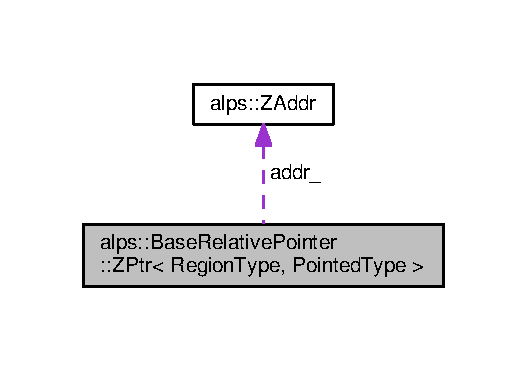
\includegraphics[width=253pt]{classalps_1_1BaseRelativePointer_1_1ZPtr__coll__graph}
\end{center}
\end{figure}
\subsection*{Public Types}
\begin{DoxyCompactItemize}
\item 
typedef Pointed\+Type $\ast$ {\bfseries pointer}\hypertarget{classalps_1_1BaseRelativePointer_1_1ZPtr_abf43f5fd49f1c4bc0e4a11d46d60a5f7}{}\label{classalps_1_1BaseRelativePointer_1_1ZPtr_abf43f5fd49f1c4bc0e4a11d46d60a5f7}

\item 
typedef boost\+::add\+\_\+reference$<$ Pointed\+Type $>$\+::type {\bfseries reference}\hypertarget{classalps_1_1BaseRelativePointer_1_1ZPtr_ab66ca9ef28e93077f43b7ba0ee7a5b48}{}\label{classalps_1_1BaseRelativePointer_1_1ZPtr_ab66ca9ef28e93077f43b7ba0ee7a5b48}

\end{DoxyCompactItemize}
\subsection*{Public Member Functions}
\begin{DoxyCompactItemize}
\item 
{\bfseries Z\+Ptr} (\hyperlink{structalps_1_1ZAddr}{Z\+Addr} zaddr)\hypertarget{classalps_1_1BaseRelativePointer_1_1ZPtr_a3ecb59de4427a4d0281c61600dbf6b3d}{}\label{classalps_1_1BaseRelativePointer_1_1ZPtr_a3ecb59de4427a4d0281c61600dbf6b3d}

\item 
{\bfseries Z\+Ptr} (Region\+Id region\+\_\+id, Linear\+Addr offset)\hypertarget{classalps_1_1BaseRelativePointer_1_1ZPtr_a0128650f250004203b83603384ec84cd}{}\label{classalps_1_1BaseRelativePointer_1_1ZPtr_a0128650f250004203b83603384ec84cd}

\item 
{\bfseries Z\+Ptr} (const \hyperlink{classalps_1_1BaseRelativePointer_1_1ZPtr}{Z\+Ptr}$<$ Region\+Type, void $>$ \&other)\hypertarget{classalps_1_1BaseRelativePointer_1_1ZPtr_a1549b21bae1523032289aca8068a1443}{}\label{classalps_1_1BaseRelativePointer_1_1ZPtr_a1549b21bae1523032289aca8068a1443}

\item 
{\bfseries Z\+Ptr} (const typename Region\+Type\+::template \hyperlink{classalps_1_1BaseRelativePointer_1_1TPtr}{T\+Ptr}$<$ Pointed\+Type $>$ \&tptr)\hypertarget{classalps_1_1BaseRelativePointer_1_1ZPtr_a6fee847bab1b7ddaf29b3cecb298964a}{}\label{classalps_1_1BaseRelativePointer_1_1ZPtr_a6fee847bab1b7ddaf29b3cecb298964a}

\item 
\hyperlink{classalps_1_1BaseRelativePointer_1_1ZPtr}{Z\+Ptr} \& {\bfseries operator=} (const typename Region\+Type\+::template \hyperlink{classalps_1_1BaseRelativePointer_1_1TPtr}{T\+Ptr}$<$ Pointed\+Type $>$ \&tptr)\hypertarget{classalps_1_1BaseRelativePointer_1_1ZPtr_a911469805adc08046344d7215a9d8a71}{}\label{classalps_1_1BaseRelativePointer_1_1ZPtr_a911469805adc08046344d7215a9d8a71}

\item 
{\bfseries operator T\+Ptr$<$ Region\+Type, Pointed\+Type $>$} ()\hypertarget{classalps_1_1BaseRelativePointer_1_1ZPtr_a0148a9e9ddedc851890e46e437c5b5ba}{}\label{classalps_1_1BaseRelativePointer_1_1ZPtr_a0148a9e9ddedc851890e46e437c5b5ba}

\end{DoxyCompactItemize}
\subsection*{Public Attributes}
\begin{DoxyCompactItemize}
\item 
\hyperlink{structalps_1_1ZAddr}{Z\+Addr} {\bfseries addr\+\_\+}\hypertarget{classalps_1_1BaseRelativePointer_1_1ZPtr_a3adf23e694b99b04819f6d00abde040a}{}\label{classalps_1_1BaseRelativePointer_1_1ZPtr_a3adf23e694b99b04819f6d00abde040a}

\end{DoxyCompactItemize}


The documentation for this class was generated from the following file\+:\begin{DoxyCompactItemize}
\item 
/home/yuan/\+Benchmarks/whisper/mnemosyne-\/gcc/usermode/library/pmalloc/include/alps/include/alps/pegasus/pointer.\+hh\end{DoxyCompactItemize}

%--- End generated contents ---

% Index
\backmatter
\newpage
\phantomsection
\clearemptydoublepage
\addcontentsline{toc}{chapter}{Index}
\printindex

\end{document}
